%% 该模板修改自《计算机学报》latex 模板
%% 主要是将双栏改成单栏,去掉了部分计算机学报标识;
%% 源文件自:https://www.overleaf.com/latex/templates/latextemplet-cjc-xelatex/ybmmymncrrmw
%% 
%%
%% This is file `CjC_template_tex.tex',
%% is modified by Zhi Wang (zhiwang@ieee.org) based on the template 
%% provided by Chinese Journal of Computers (http://cjc.ict.ac.cn/).
%%
%% This version is capable with Overleaf (XeLaTeX).
%%
%% Update date: 2023/03/10
%% -------------------------------------------------------------------
%% Copyright (C) 2016--2023 
%% -------------------------------------------------------------------
%% This file may be distributed and/or modified under the
%% conditions of the LaTeX Project Public License, either version 1.3c
%% of this license or (at your option) any later version.
%% The latest version of this license is in
%%    https://www.latex-project.org/lppl.txt
%% and version 1.3c or later is part of all distribution`s of LaTeX
%% version 2008 or later.
%% -------------------------------------------------------------------

\documentclass[10.5pt,compsoc,UTF8]{CjC}
\usepackage{CTEX}
\usepackage{graphicx}
\usepackage{footmisc}
\usepackage{subfigure}
\usepackage{url}
\usepackage{multirow}
\usepackage{multicol}
\usepackage[noadjust]{cite}
\usepackage{amsmath,amsthm}
\usepackage{amssymb,amsfonts}
\usepackage{booktabs}
\usepackage{color}
\usepackage{ccaption}
\usepackage{booktabs}
\usepackage{float}
\usepackage{fancyhdr}
\usepackage{caption}
\usepackage{xcolor,stfloats}
\usepackage{comment}
\setcounter{page}{1}
\graphicspath{{figures/}}
\usepackage{cuted}%flushend,
\usepackage{captionhack}
\usepackage{epstopdf}
\usepackage{gbt7714}
\usepackage{listings}
\usepackage{xeCJK}
\usepackage{float}
\usepackage{sourcecodepro}
\usepackage[T1]{fontenc}
\usepackage{hyperref}

\setmainfont{Times Roman}
% \setCJKmainfont{Noto Sans Mono CJK TC}
\setCJKmainfont{標楷體.ttc}
\setmonofont{Cascadia Code}

%===============================%

\headevenname{\mbox{\quad} \hfill  \mbox{\zihao{-5}{ \hfill 2024 Hardware Design  } \hspace {50mm} \mbox{2024 年 11 月}}}%
\headoddname{Group 21 \hfill Lab 5: Keyboard and Audio Modules}%

%footnote use of *
\renewcommand{\thefootnote}{\fnsymbol{footnote}}
\setcounter{footnote}{0}
\renewcommand\footnotelayout{\zihao{5-}}

\newtheoremstyle{mystyle}{0pt}{0pt}{\normalfont}{1em}{\bf}{}{1em}{}
\theoremstyle{mystyle}
\renewcommand\figurename{figure~}
\renewcommand{\thesubfigure}{(\alph{subfigure})}
\newcommand{\upcite}[1]{\textsuperscript{\cite{#1}}}
\renewcommand{\labelenumi}{(\arabic{enumi})}
\newcommand{\tabincell}[2]{\begin{tabular}{@{}#1@{}}#2\end{tabular}}
\newcommand{\abc}{\color{white}\vrule width 2pt}
\renewcommand{\bibsection}{}
\makeatletter
\renewcommand{\@biblabel}[1]{[#1]\hfill}
\makeatother
\setlength\parindent{2em}
%\renewcommand{\hth}{\begin{CJK*}{UTF8}{gbsn}}
%\renewcommand{\htss}{\begin{CJK*}{UTF8}{gbsn}}
\renewcommand{\contentsname}{Table of Contents}

\begin{document}

\hyphenpenalty=50000
\makeatletter
\newcommand\mysmall{\@setfontsize\mysmall{7}{9.5}}
\newenvironment{tablehere}
  {\def\@captype{table}}

\let\temp\footnote
\renewcommand \footnote[1]{\temp{\zihao{-5}#1}}

\hypersetup{
  colorlinks=false,
  pdfborder={0 0 0},
}

\thispagestyle{plain}%
\thispagestyle{empty}%
\pagestyle{CjCheadings}

% \begin{table*}[!t]
\vspace {-13mm}


\onecolumn
\zihao{5-}\noindent Group 21 \hfill Lab 5: Keyboard and Audio Modules \hfill 2024 年 11 月\\
\noindent\rule[0.25\baselineskip]{\textwidth}{1pt}


\begin{center}
    \vspace {11mm}
    {\zihao{2} \heiti \fangsong Lab 5: Keyboard and Audio Modules}
    
    \vskip 5mm
    
    {\zihao{4}\fangsong Group 21: 陳克盈(112062205)、蔡明妡(112062224)}
\end{center}

\lstset{
    % backgroundcolor=\color{red!50!green!50!blue!50},%程式碼塊背景色為淺灰色
    rulesepcolor= \color{gray}, %程式碼塊邊框顏色
    breaklines=true,  %程式碼過長則換行
    numbers=left, %行號在左側顯示
    numberstyle= \small\ttfamily,%行號字型
    keywordstyle= \color{blue},%關鍵字顏色
    commentstyle=\color{gray}, %註釋顏色
    frame=shadowbox%用方框框住程式碼塊
    basicstyle=\ttfamily\footnotesize,
}
 
\definecolor{improvecolor}{rgb}{0,0.6,0} % 深綠色
\definecolor{declinecolor}{rgb}{0.6,0,0} % 深紅色


%%%%%%%%%%%%%%%%%%%%%%%%%%%%%%%%%%%%%%
\zihao{5}
\vskip 10mm
% \begin{multicols}{1}


%%%%%%%%%%%%%%%%%%%%%%%%%%%%%%%%%%%%%%%%%%
%%%%%%%%%%%%%%%%%%%%%%%%%%%%%%%%%%%%%%%%%%

\tableofcontents
\newpage

\section{Q1: Sliding Windows sequence detactor}

\begin{itemize}
  \item input clk: clock
  \item input rst\_n: reset
  \item input in: input data
  \item output dec: detect signal
\end{itemize}

這題需要我們實作一個 Mealy maching,用來偵測輸入的序列是不是滿足 $1110(01)+11$ 這個 regular expression。

\subsection{State diagram}

首先我們需要先畫出狀態圖,狀態的定義如下:
\begin{itemize}
  \item S0: 初始狀態
  \item S1: 偵測到 1 的狀態
  \item S2: 偵測到 11 的狀態
  \item S3: 偵測到 111 的狀態,因此接受到 1 之後,還是代表前面有 111,因此會繼續保持 S3。
  \item S4: 偵測到 1110 這個狀態,因此接收到 1 之後,會回到只接收 1 的狀態,也就是 S1
  \item S5: 偵測到 11100 的狀態,由於下一個狀態 S6 需要輸入 1 才會達到,因此當輸入 0 的時候就必須回到 S0 的狀態
  \item S6: 偵測到 111001 的狀態,由於 (01) 可以多次出現,因此輸入為 0 的時候,可以回到 S5 重新偵測 (01)。
  \item S7: 偵測到 1110(01)+1 的狀態,如果輸入為 1,就代表符合 regular expression,\
            但因為這個 detector 是 Sliding Window 的,不會因為偵測到符合的 sequence 就直接重設,\
            因此輸入 1 之後會再回到 S3。
\end{itemize}

\newpage

\begin{figure}[h!]
  \centering
  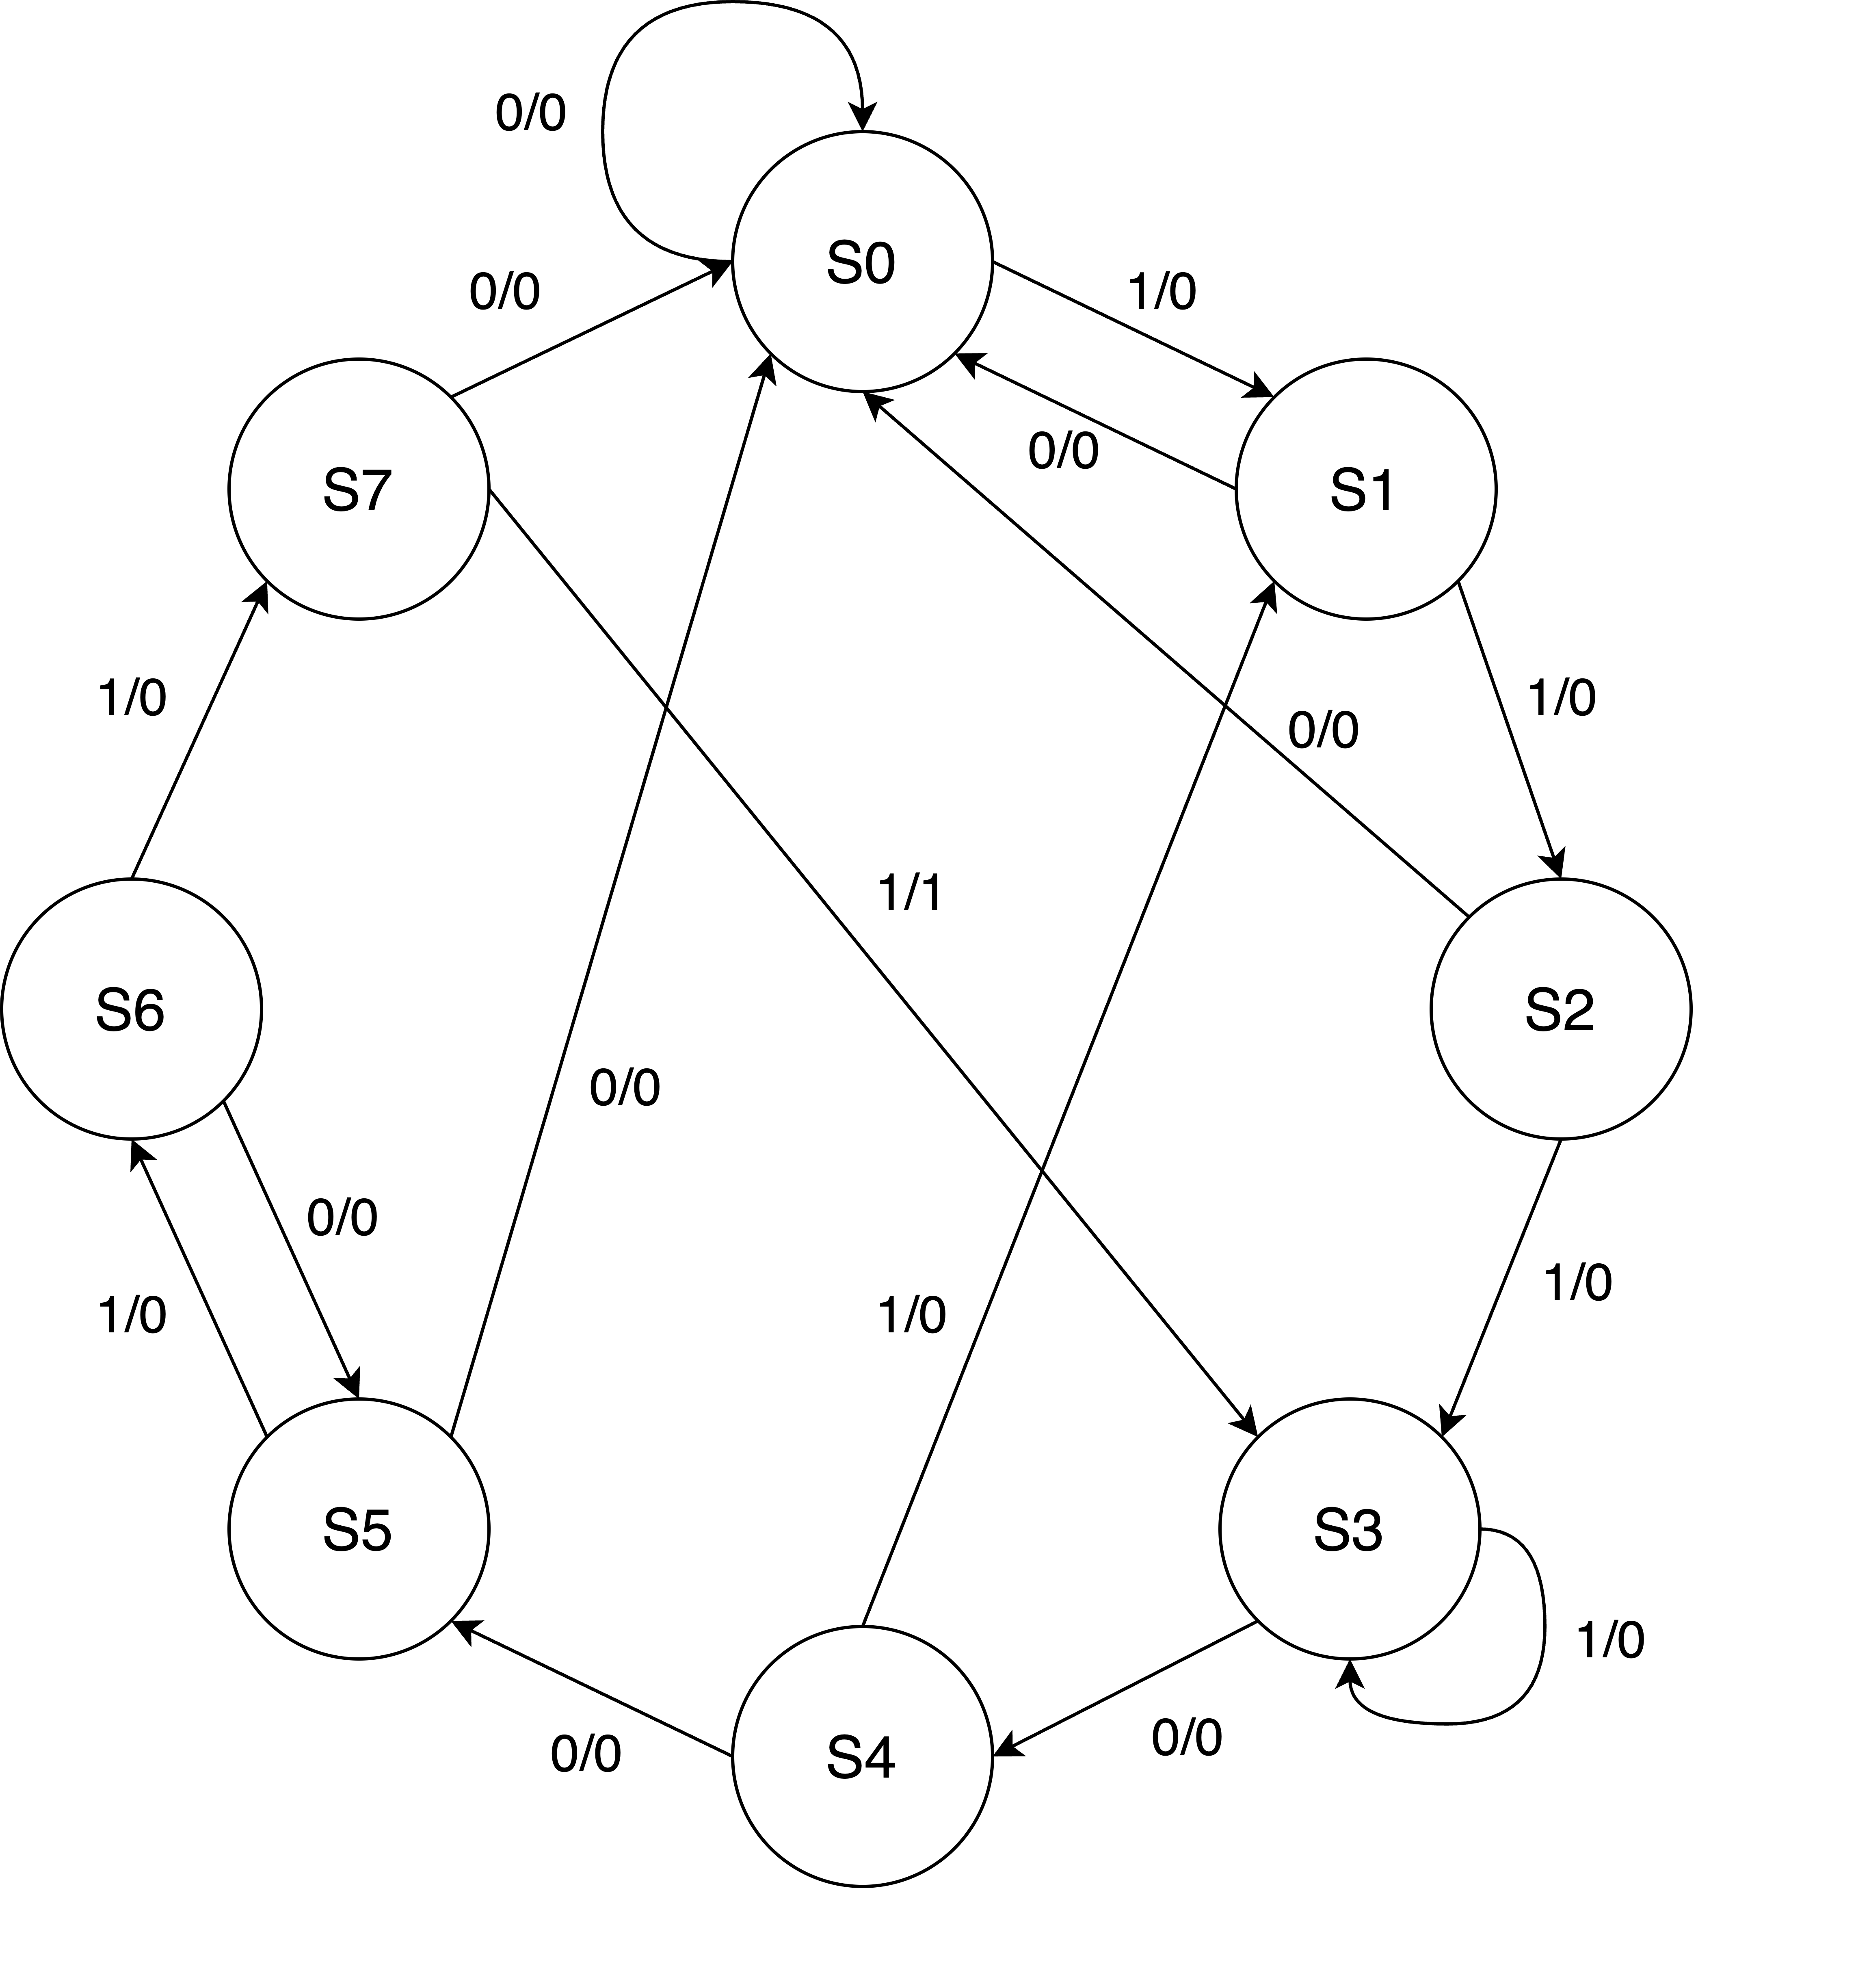
\includegraphics[width=0.6\textwidth]{./img/Q1-state.png}
  \caption{Q1 State diagram}
  \label{fig:Q1-state}
\end{figure}

\subsection{Implementation}
首先是狀態偵測的部分,我們使用 switch case 的語法,針對目前的狀態以及輸入的值,來決定下一個狀態。\
另外,因為這是一個 Mealy maching,dec 的值是不受 clock 影響的,因此 dec 是額外計算的,只要當前狀態是 S7,\
且輸入是 1,就會馬上輸出 True。

\begin{figure}[h!]
  \centering
  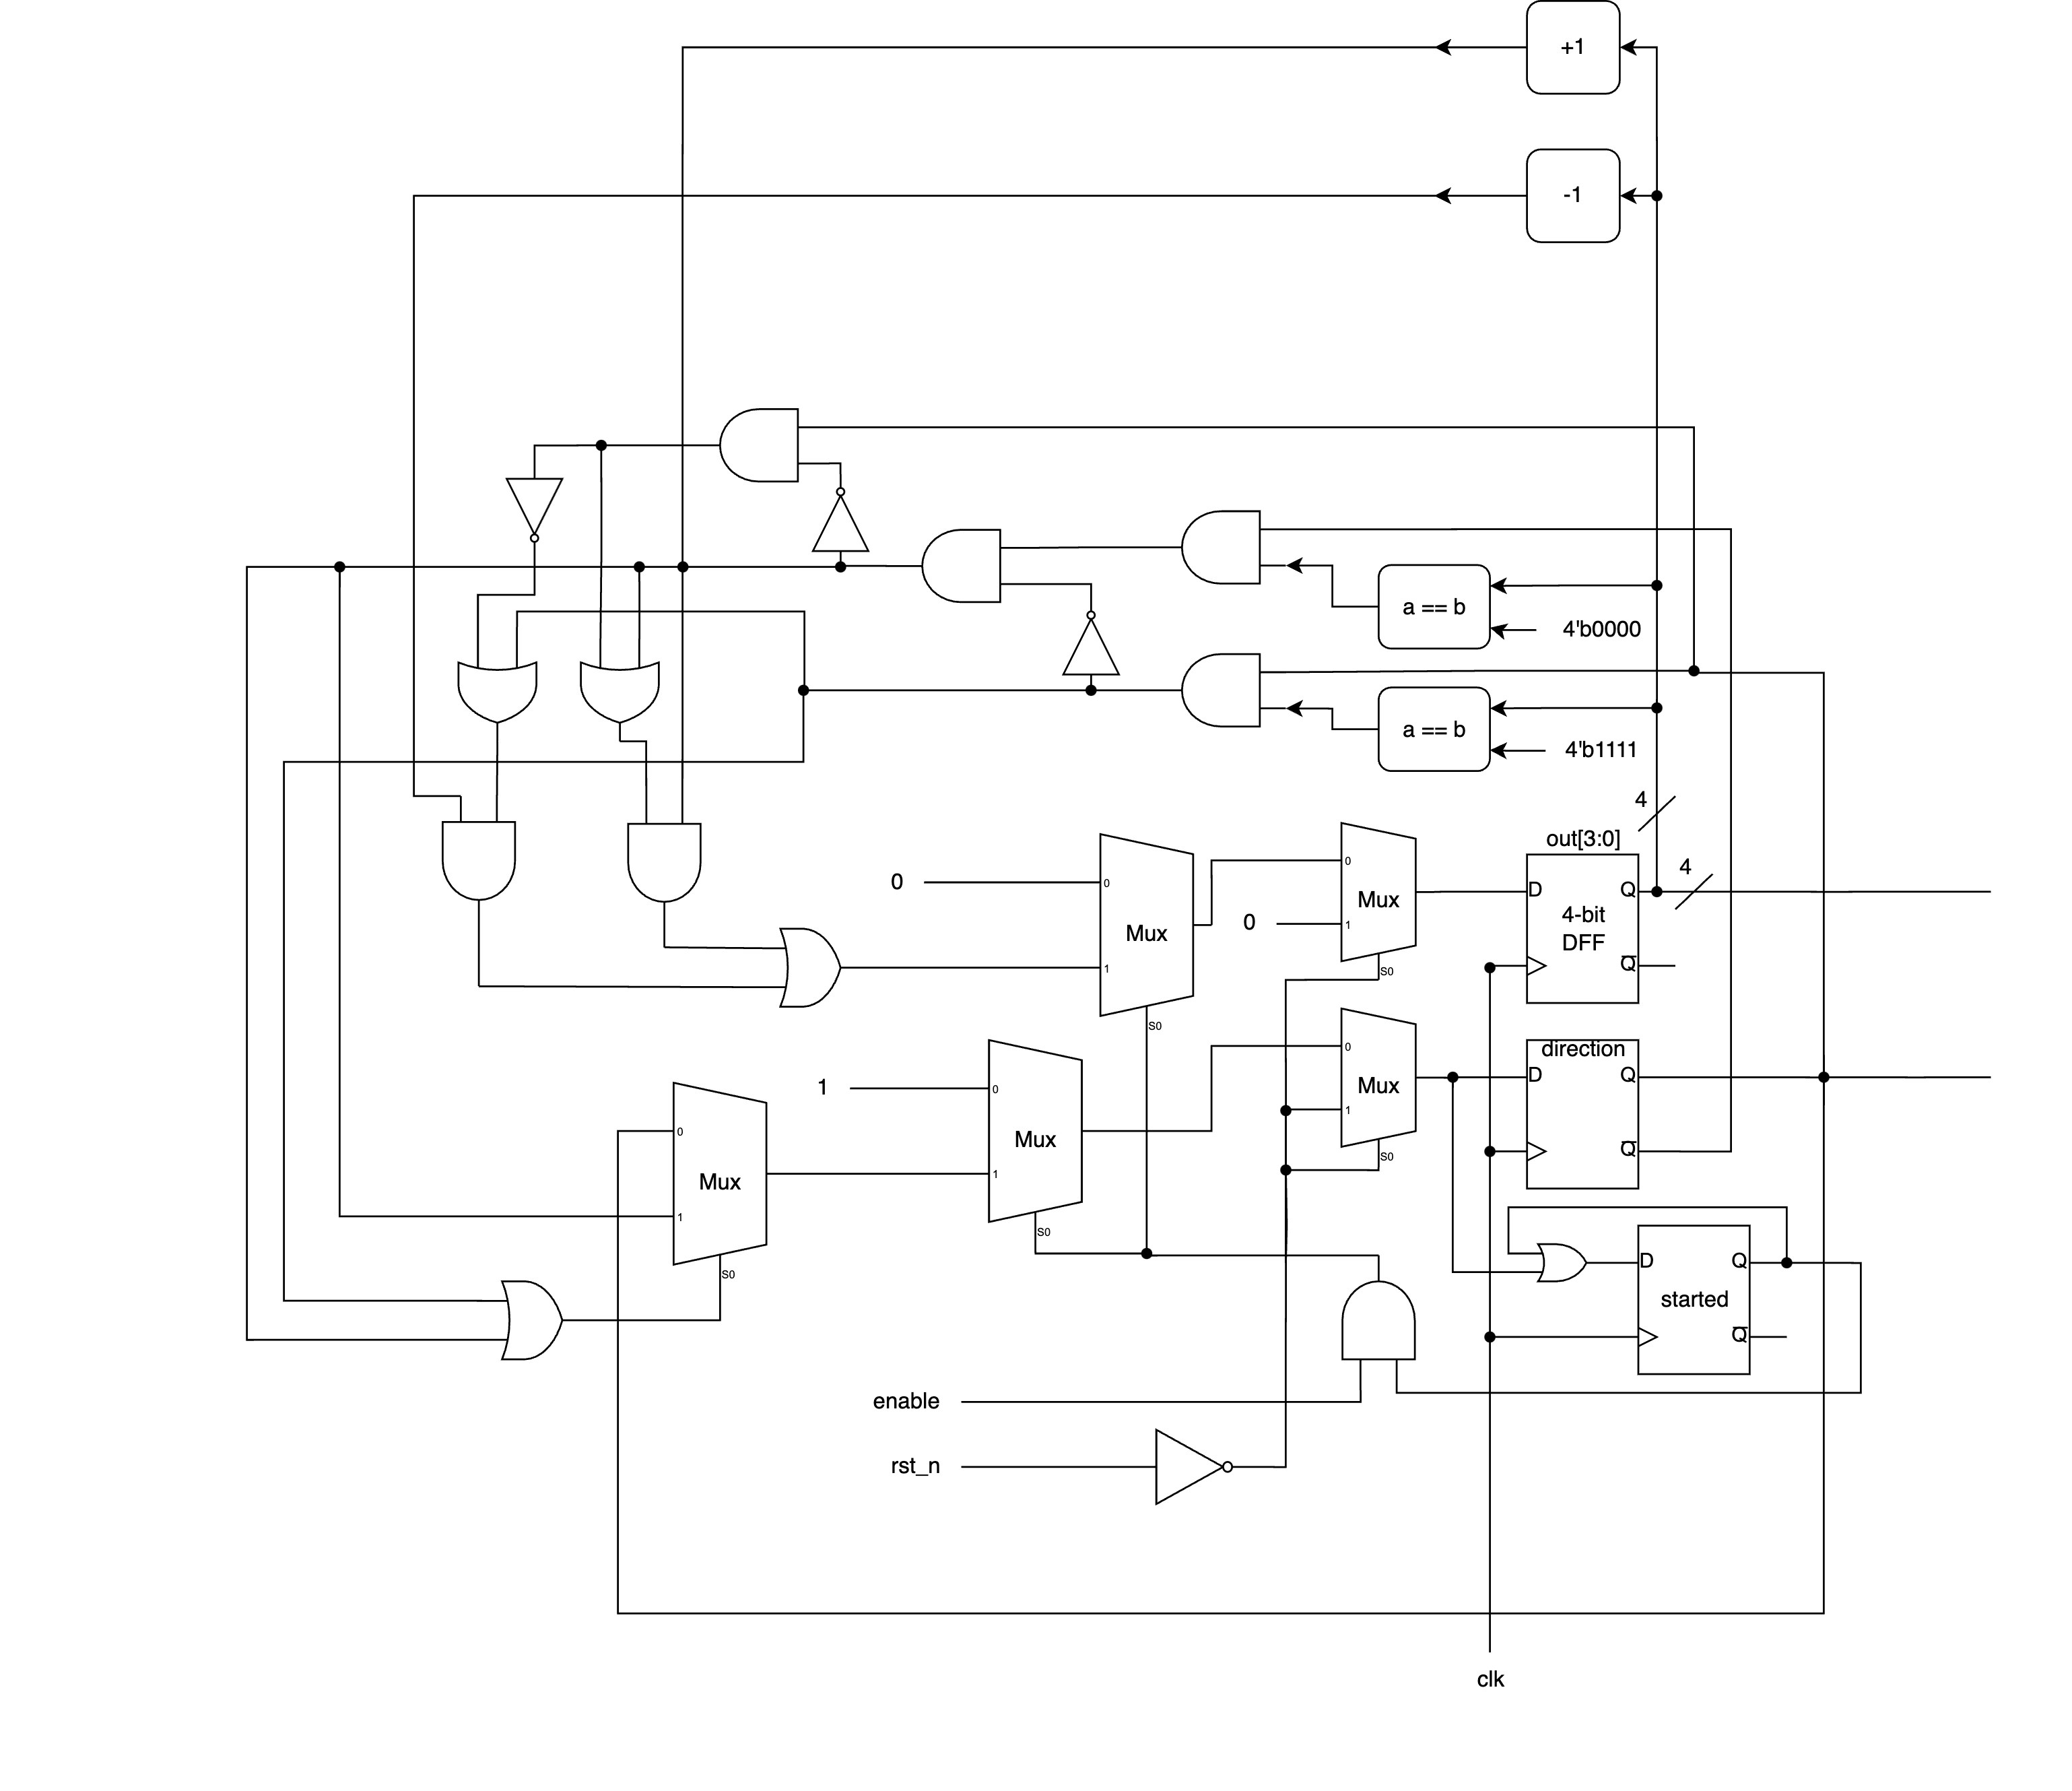
\includegraphics[width=0.6\textwidth]{./img/Q1.png}
  \caption{Q1 Circuit}
  \label{fig:Q1-circuit}
\end{figure}

\newpage

\subsection{Simulation}
我們重現了題目上的波形圖,可以發現當輸入的序列符合 regular expression 的時候,dec 會變成 1。

\begin{figure}[h!]
  \centering
  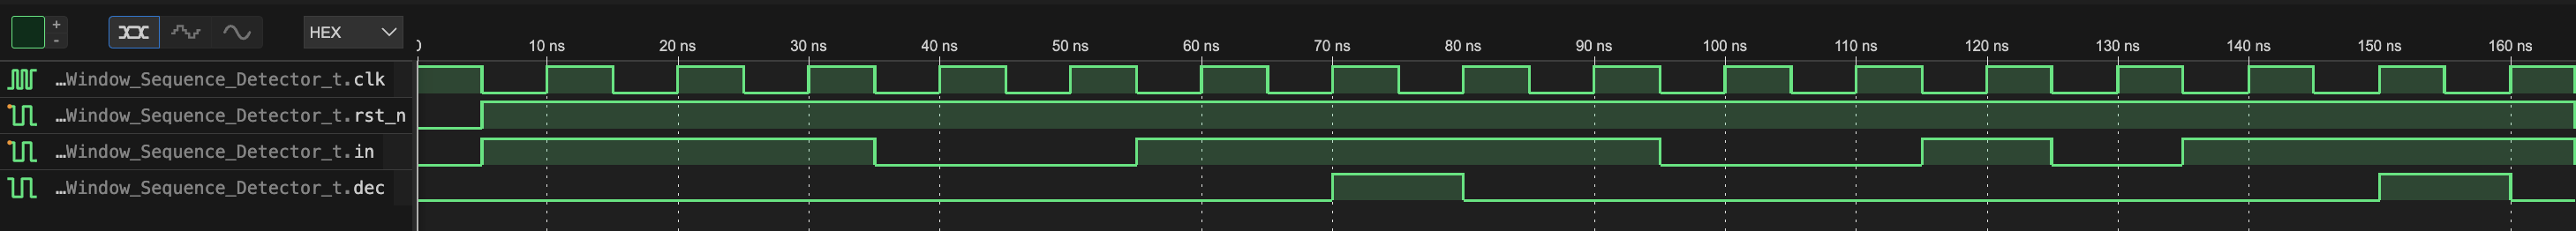
\includegraphics[width=0.8\textwidth]{./img/Q1-match.png}
  \caption{Q1 Waveform match}
  \label{fig:Q1-match}
\end{figure}

\begin{figure}[h!]
  \centering
  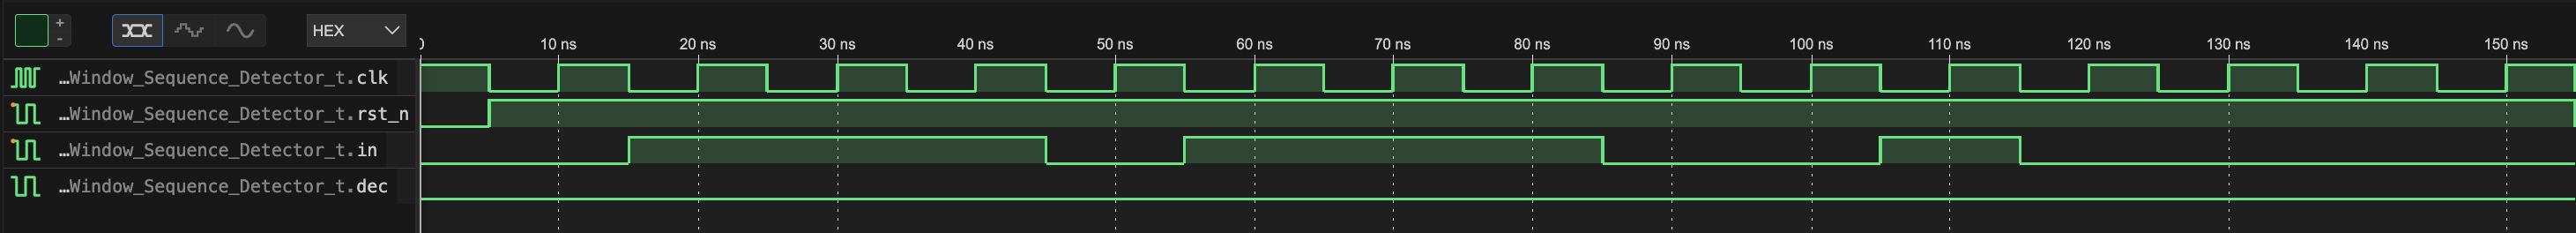
\includegraphics[width=0.8\textwidth]{./img/Q1-dismatch.png}
  \caption{Q1 Waveform dismatch}
  \label{fig:Q1-dismatch}
\end{figure}


\section{Q2: Traffic light controller}

\begin{itemize}
  \item input clk: clock
  \item input rst\_n: reset
  \item input lr\_has\_car: Local road has car
  \item output hw\_light: Highway light
  \item output lr\_light: Local road light
\end{itemize}

這題需要我們實作一個紅綠燈的控制器,控制一個由 Highway 和 Local road 兩條道路所組成的交叉路口的紅綠燈。
\par
由於 Highway 的優先度最高,因此這個流程分為六個狀態(三種顏色在程式碼中以二進位表示,Green: 100, \
Yellow: 010, Red: 001):
\begin{enumerate}
  \item HW = Green, LR = Red: 如果已經保持這個狀態 $\ge 70$ 個 cycle 以上,且 Local road 有車,\
        那就進到下一個狀態。
  \item HW = Yellow, LR = Red: 黃燈階段,保持 25 個 cycle。
  \item HW = Red, LR = Red: 兩邊都紅燈,保持一個 cycle
  \item HW = Red, LR = Green: Local road 綠燈,保持 70 個 cycle
  \item HW = Red, LR = Yellow: Local road 黃燈,保持 25 個 cycle
  \item HW = Red, LR = Red: 兩邊都紅燈,保持一個 cycle 後回到第一個狀態。
\end{enumerate}

\subsection{State diagram}
\begin{figure}[h!]
  \centering
  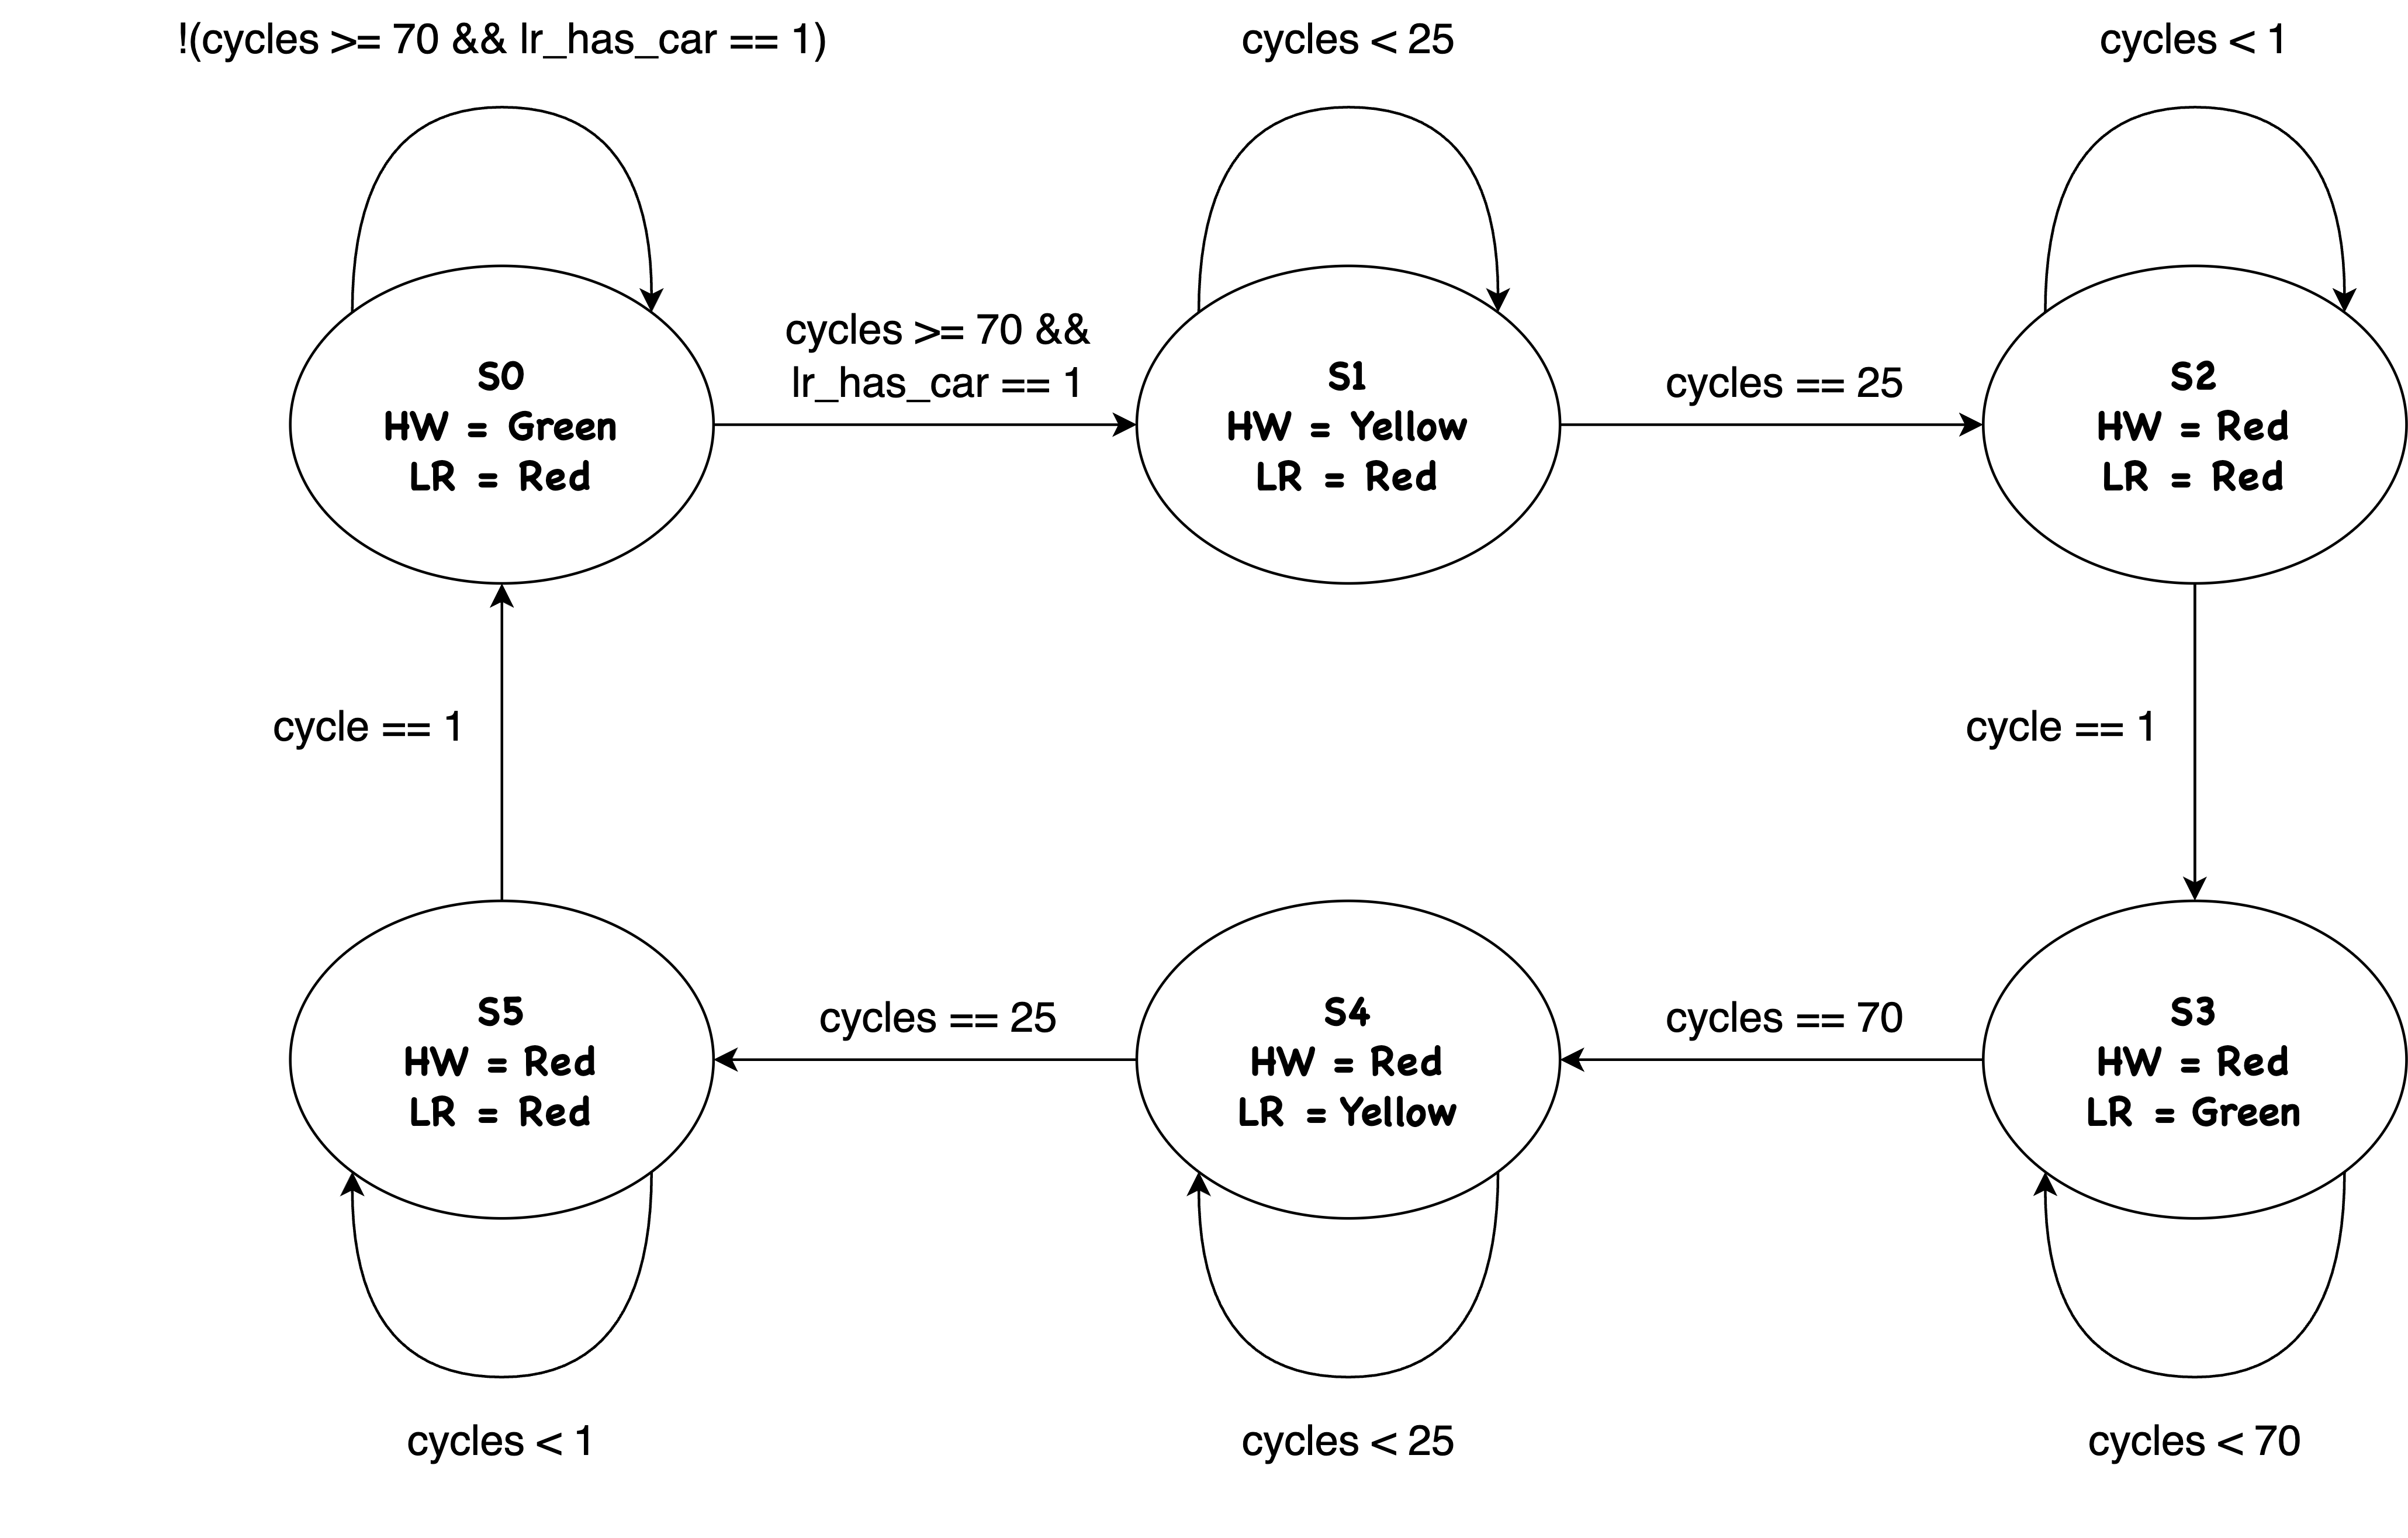
\includegraphics[width=0.6\textwidth]{./img/Q2-state.png}
  \caption{Q2 State diagram}
  \label{fig:Q2-state}
\end{figure}

\subsection{Implementation}
跟前一題的實作方法相似,使用 switch case 由目前經過的 clock cycle 以及狀態來決定下一個狀態是什麼。
\par
首先是紅綠燈的判定:
\begin{figure}[h!]
  \centering
  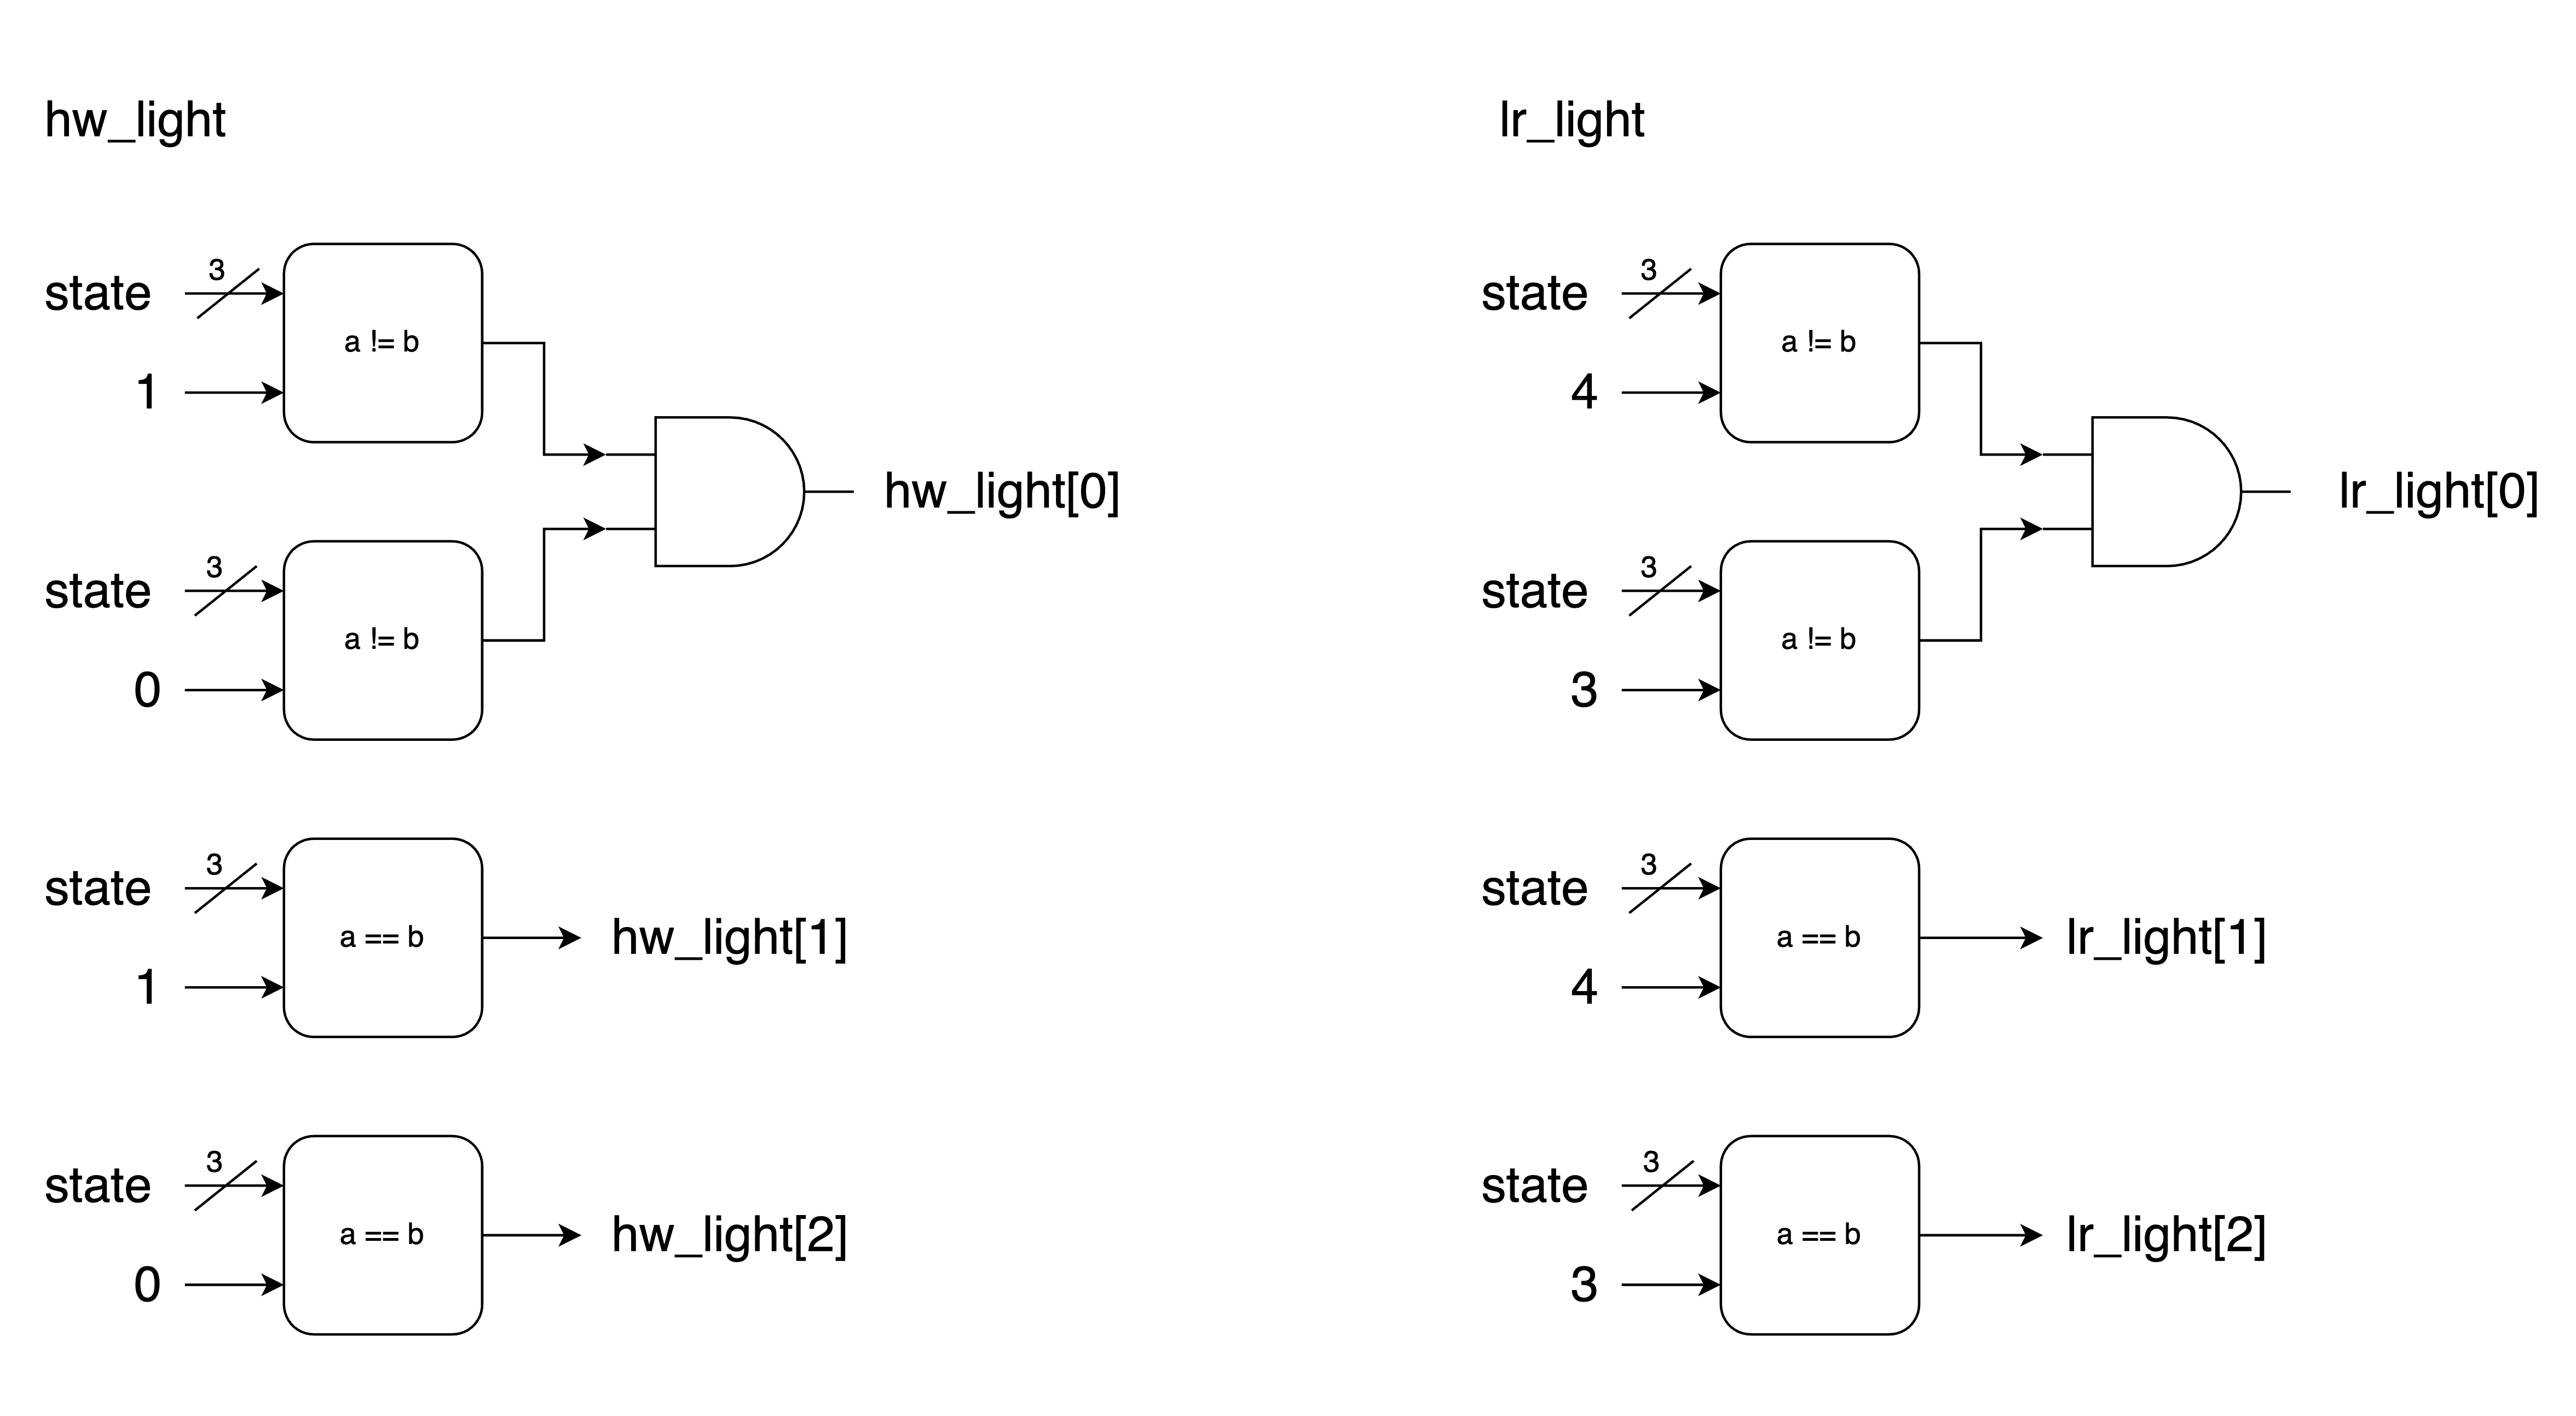
\includegraphics[width=0.5\textwidth]{./img/Q2-hwlr.png}
  \caption{Q2 Light Circuit}
  \label{fig:Q2-light}
\end{figure}

\newpage

接著是狀態的判定:
\begin{figure}[h!]
  \centering
  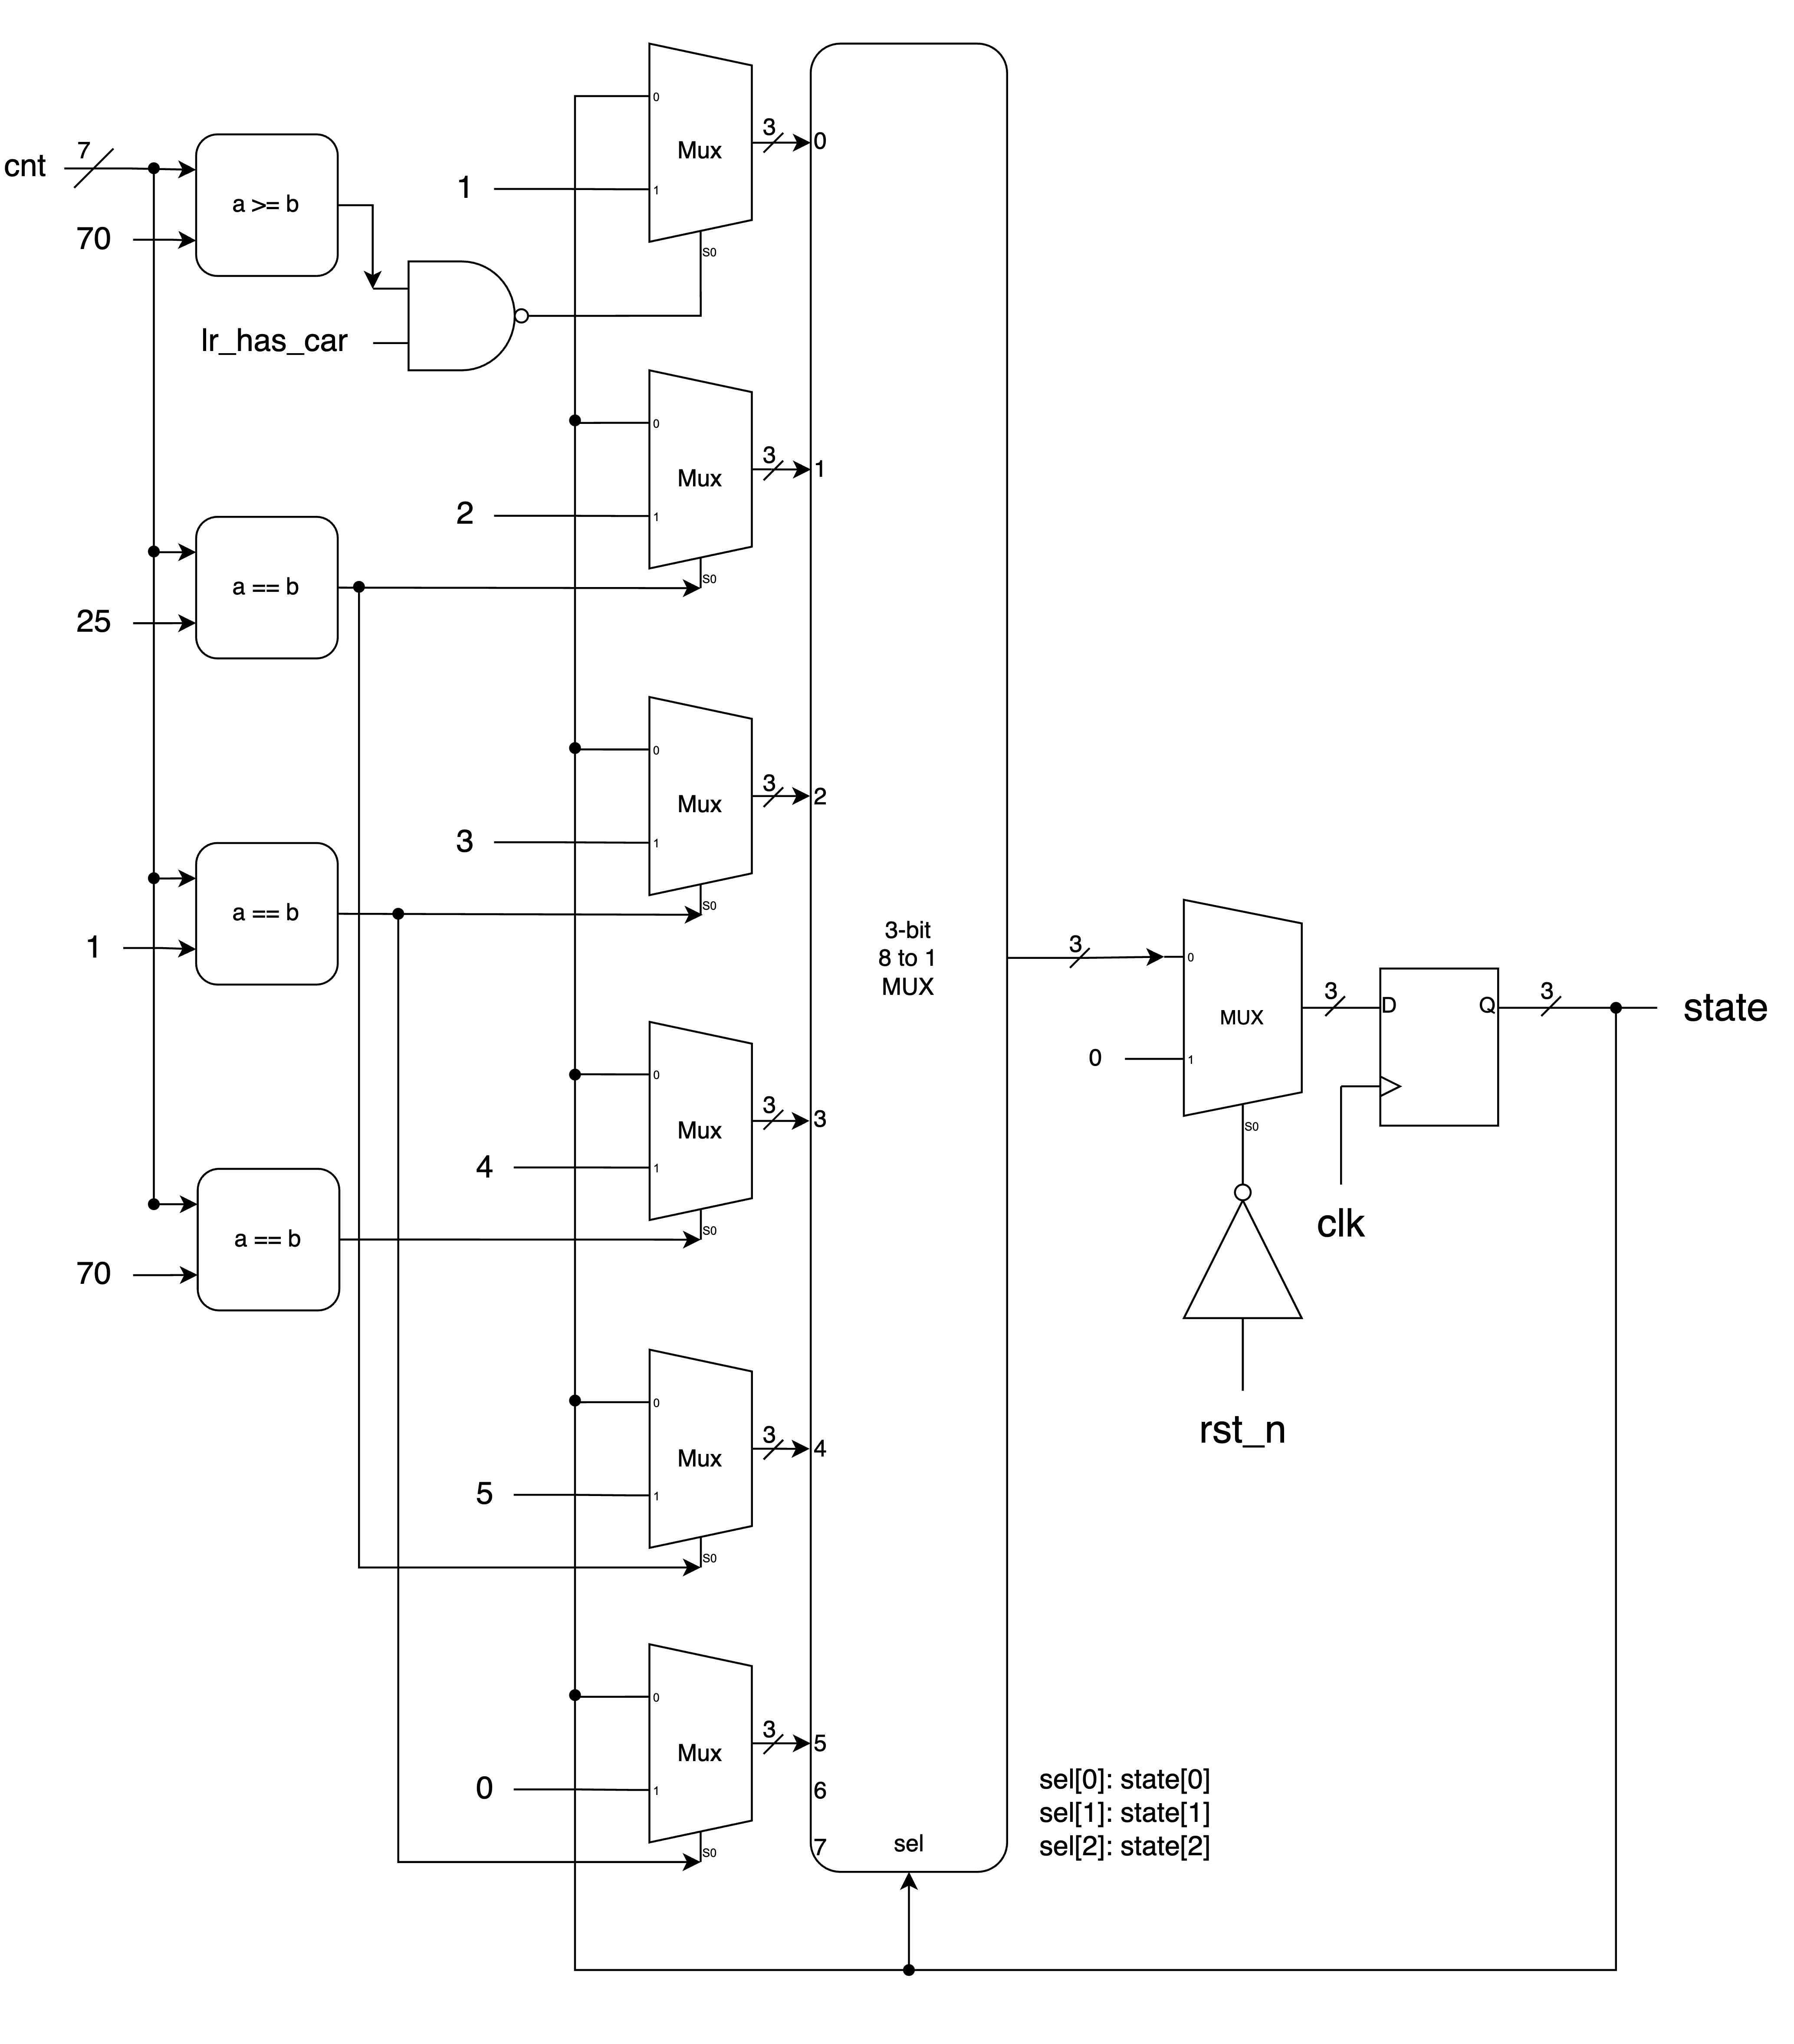
\includegraphics[width=0.7\textwidth]{./img/Q2-state-circuit.png}
  \caption{Q2 Circuit}
  \label{fig:Q2-circuit}
\end{figure}

\newpage

然後是計數器的判定:
\begin{figure}[h!]
  \centering
  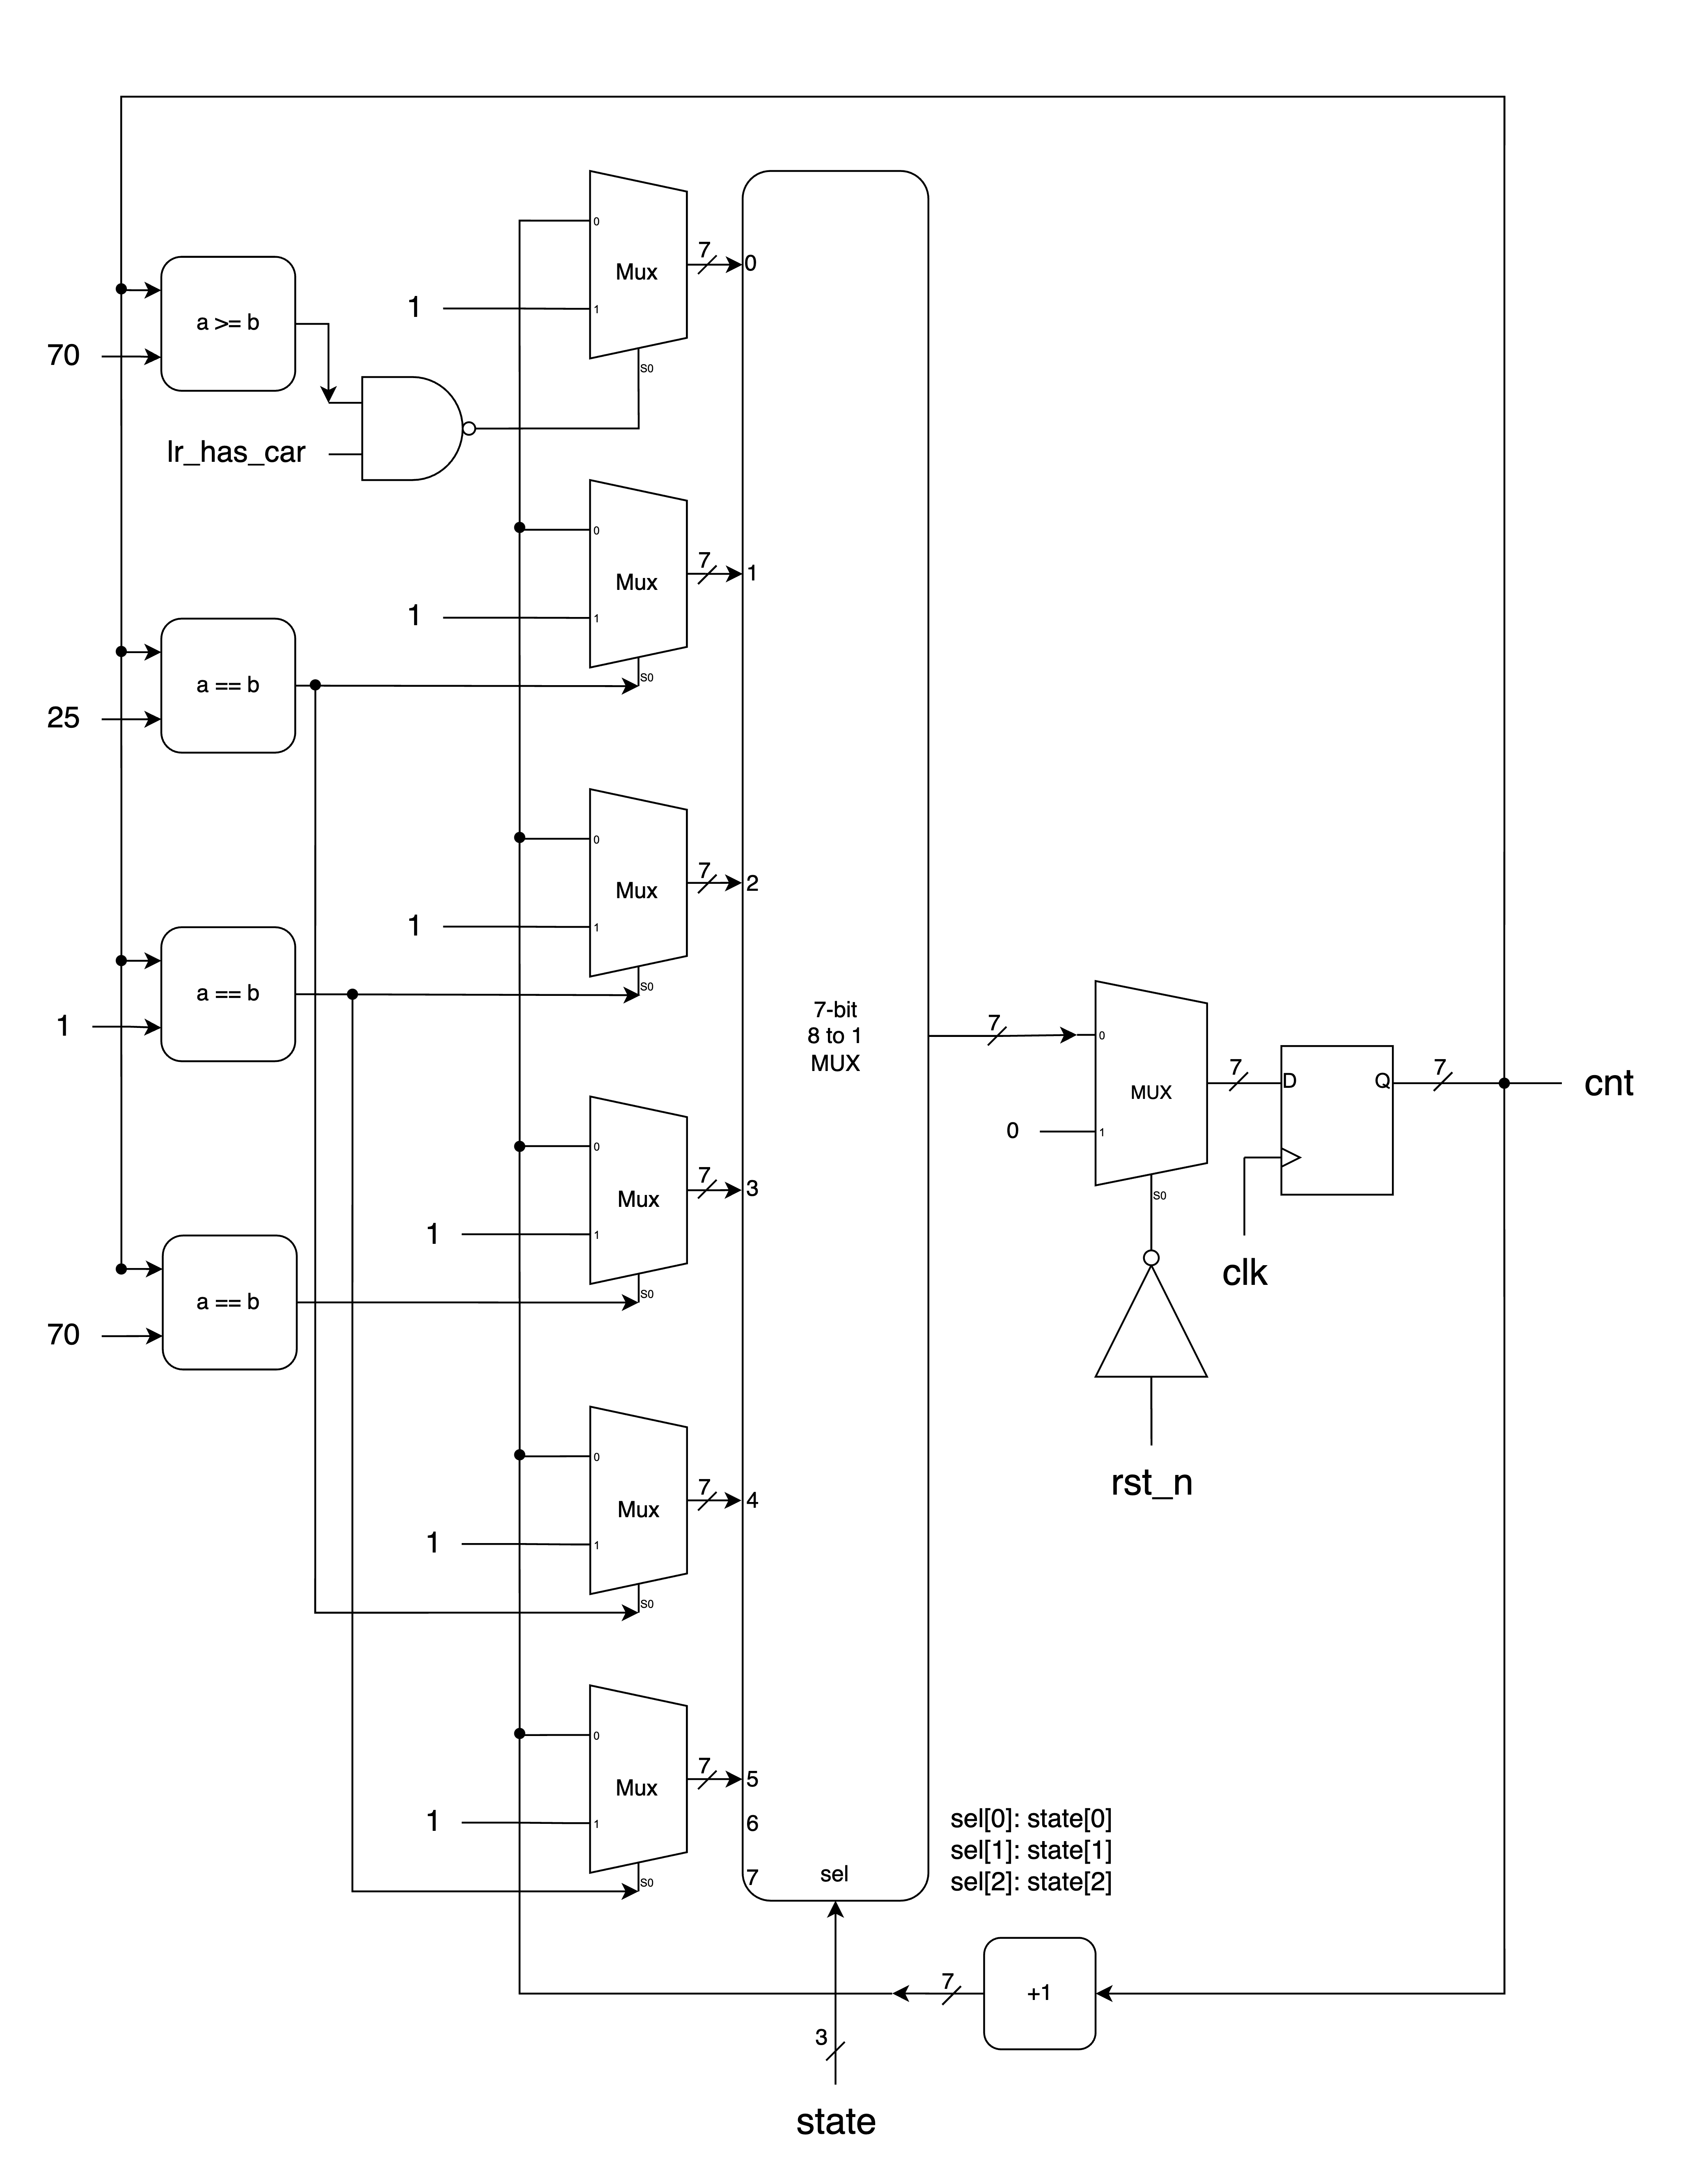
\includegraphics[width=0.8\textwidth]{./img/Q2-cnt-circuit.png}
  \caption{Q2 Counter Circuit}
  \label{fig:Q2-counter}
\end{figure}
\newpage

\subsection{Simulation}
我們重現了題目上的波形圖:

\begin{figure}[h!]
  \centering
  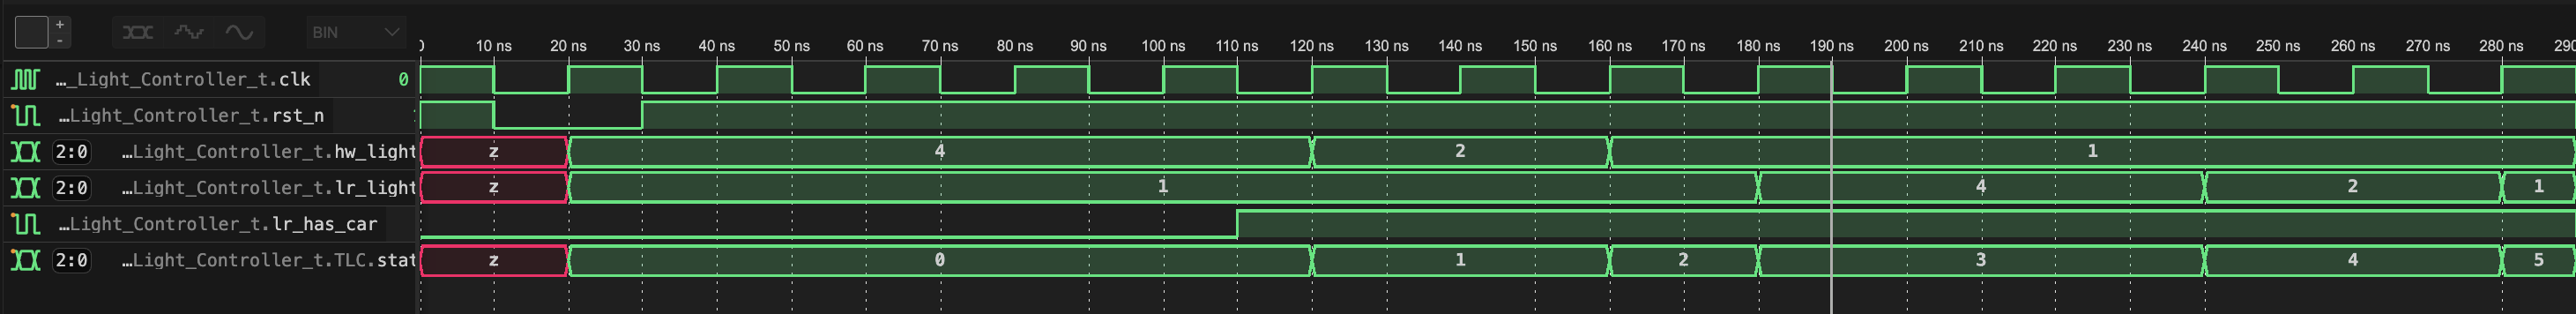
\includegraphics[width=\textwidth]{./img/Q2-tb1.png}
  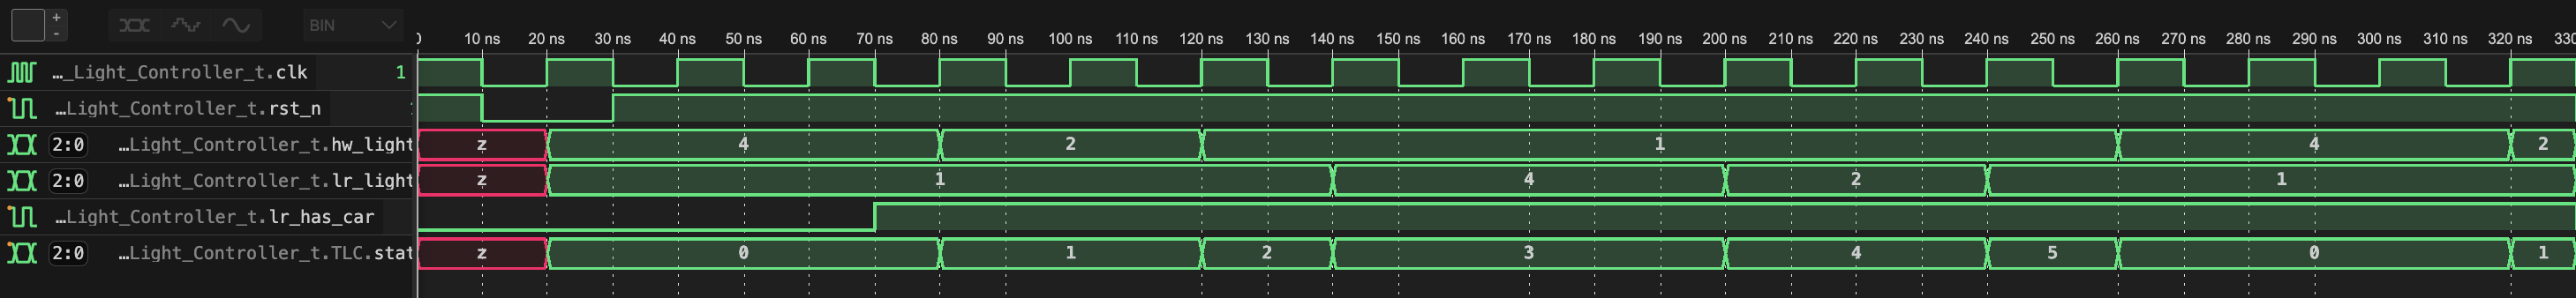
\includegraphics[width=\textwidth]{./img/Q2-tb2.png}
  \caption{Q2 Waveform}
  \label{fig:Q2-waveform}
\end{figure}


\section{Q3: Greatest common divisor}
\begin{itemize}
  \item input clk: clock
  \item input rst\_n: reset
  \item input start: start signal
  \item input [15:0] a, b: input numbers
\end{itemize}

這題我們需要實作一個利用輾轉相除法計算 GCD 的模組,\
整體分為三個狀態:
\begin{enumerate}
  \item WAIT: 等待 start signal,當收到 start signal 的時候,就 fetch 輸入的 a, b,\
        並進入到下一個狀態
  \item CAL: 利用輾轉相除法計算 GCD
  \item FINISH: 計算完比,將 gcd 輸出,在兩個 clock cycle 後回到 WAIT 狀態
\end{enumerate}

\subsection{Implementation}

首先是狀態圖:\\
% TODO: 狀態圖
\begin{figure}[h!]
    \centering
    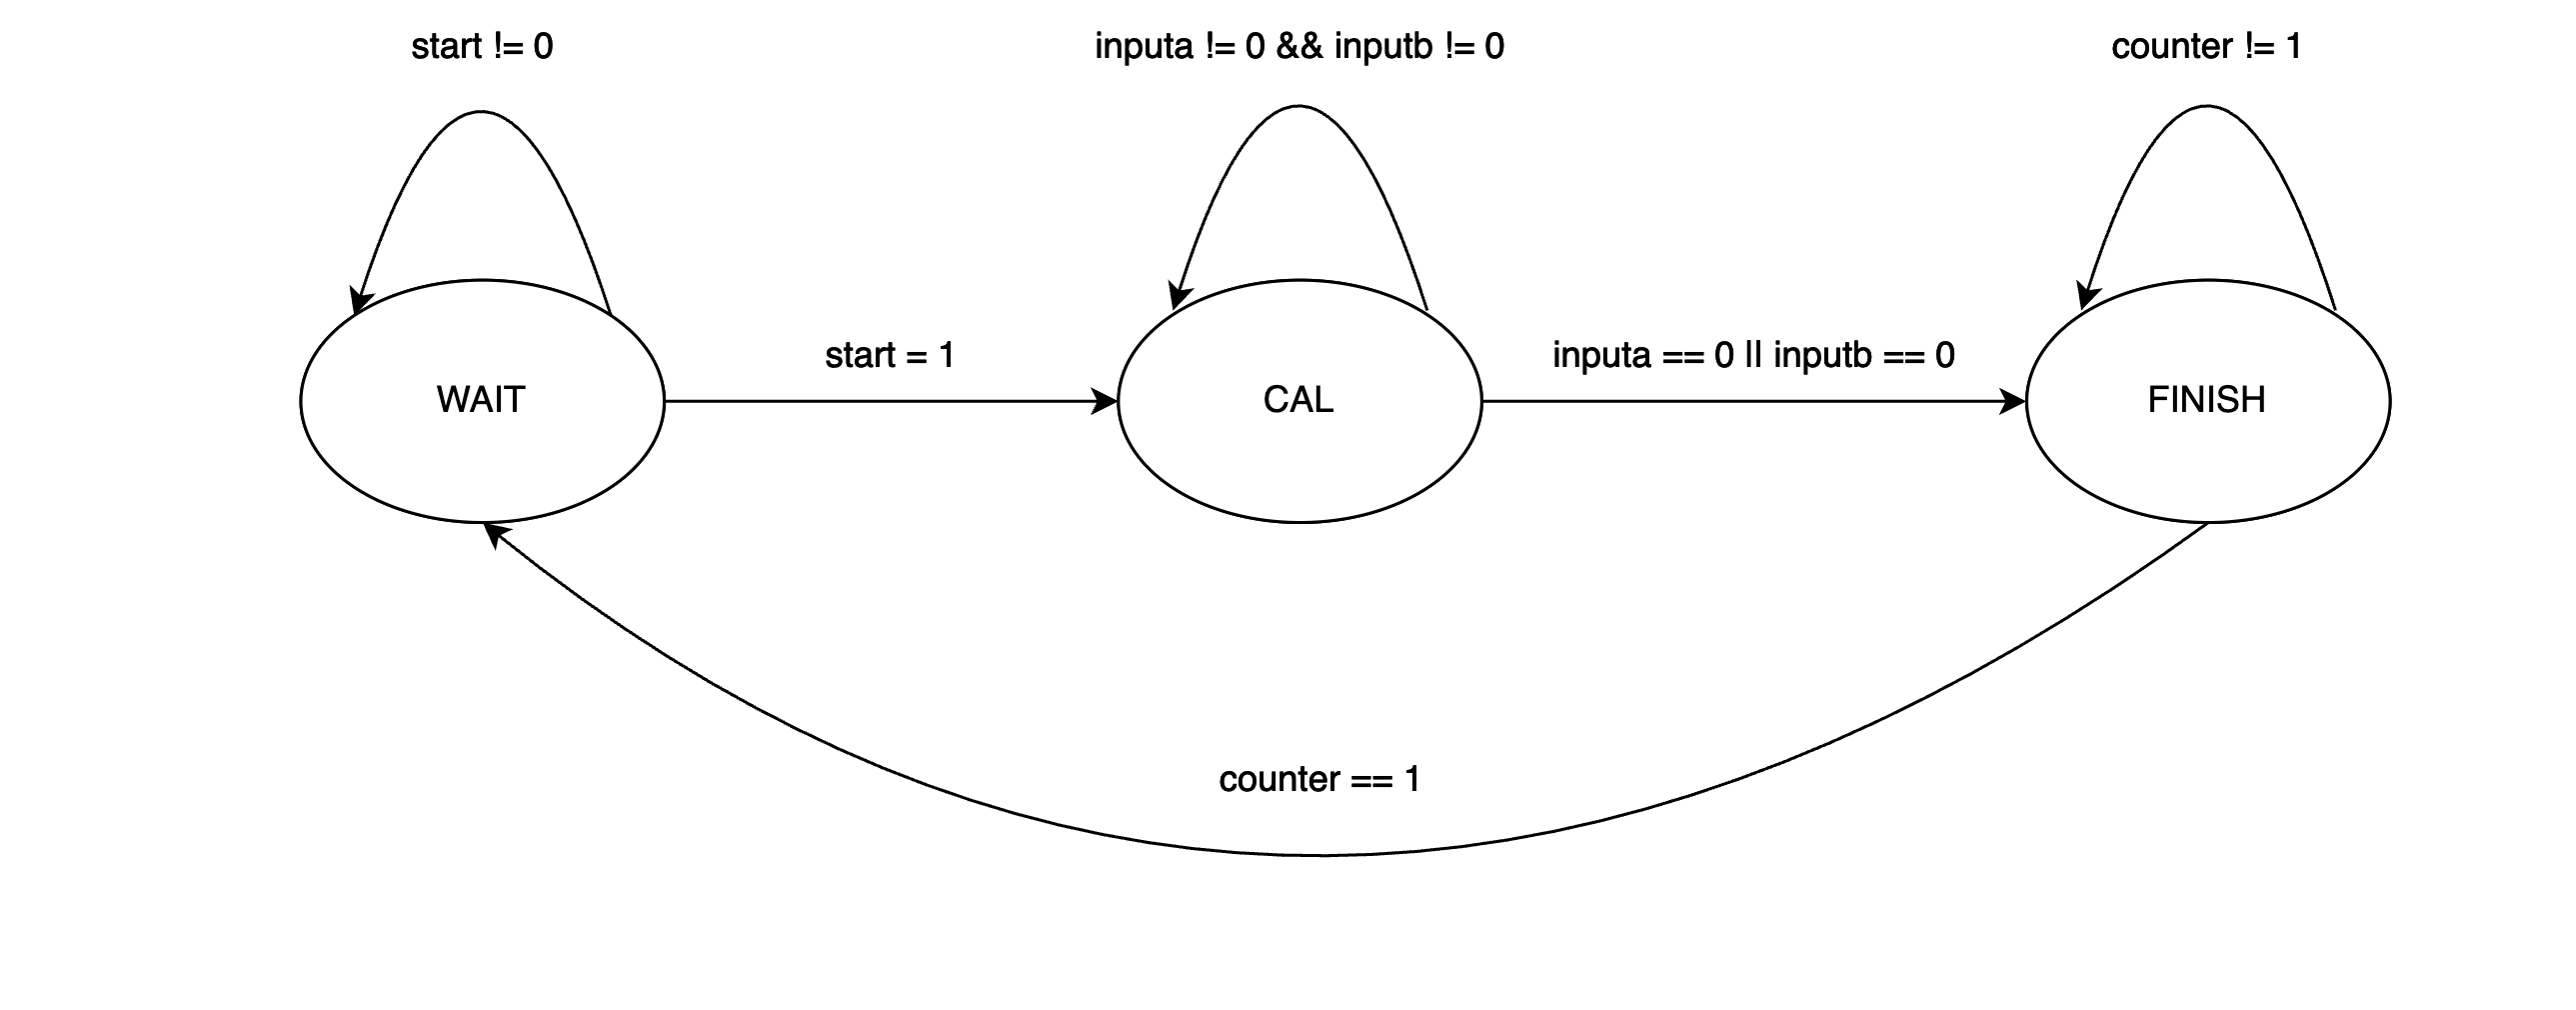
\includegraphics[width=0.6\textwidth]{./img/Q3-state.png}
    \caption{Q3 State diagram}
    \label{fig:Q3-state}
\end{figure}

\newpage

接著是計數器與狀態的判定:\\

\begin{figure}[h!]
  \centering
  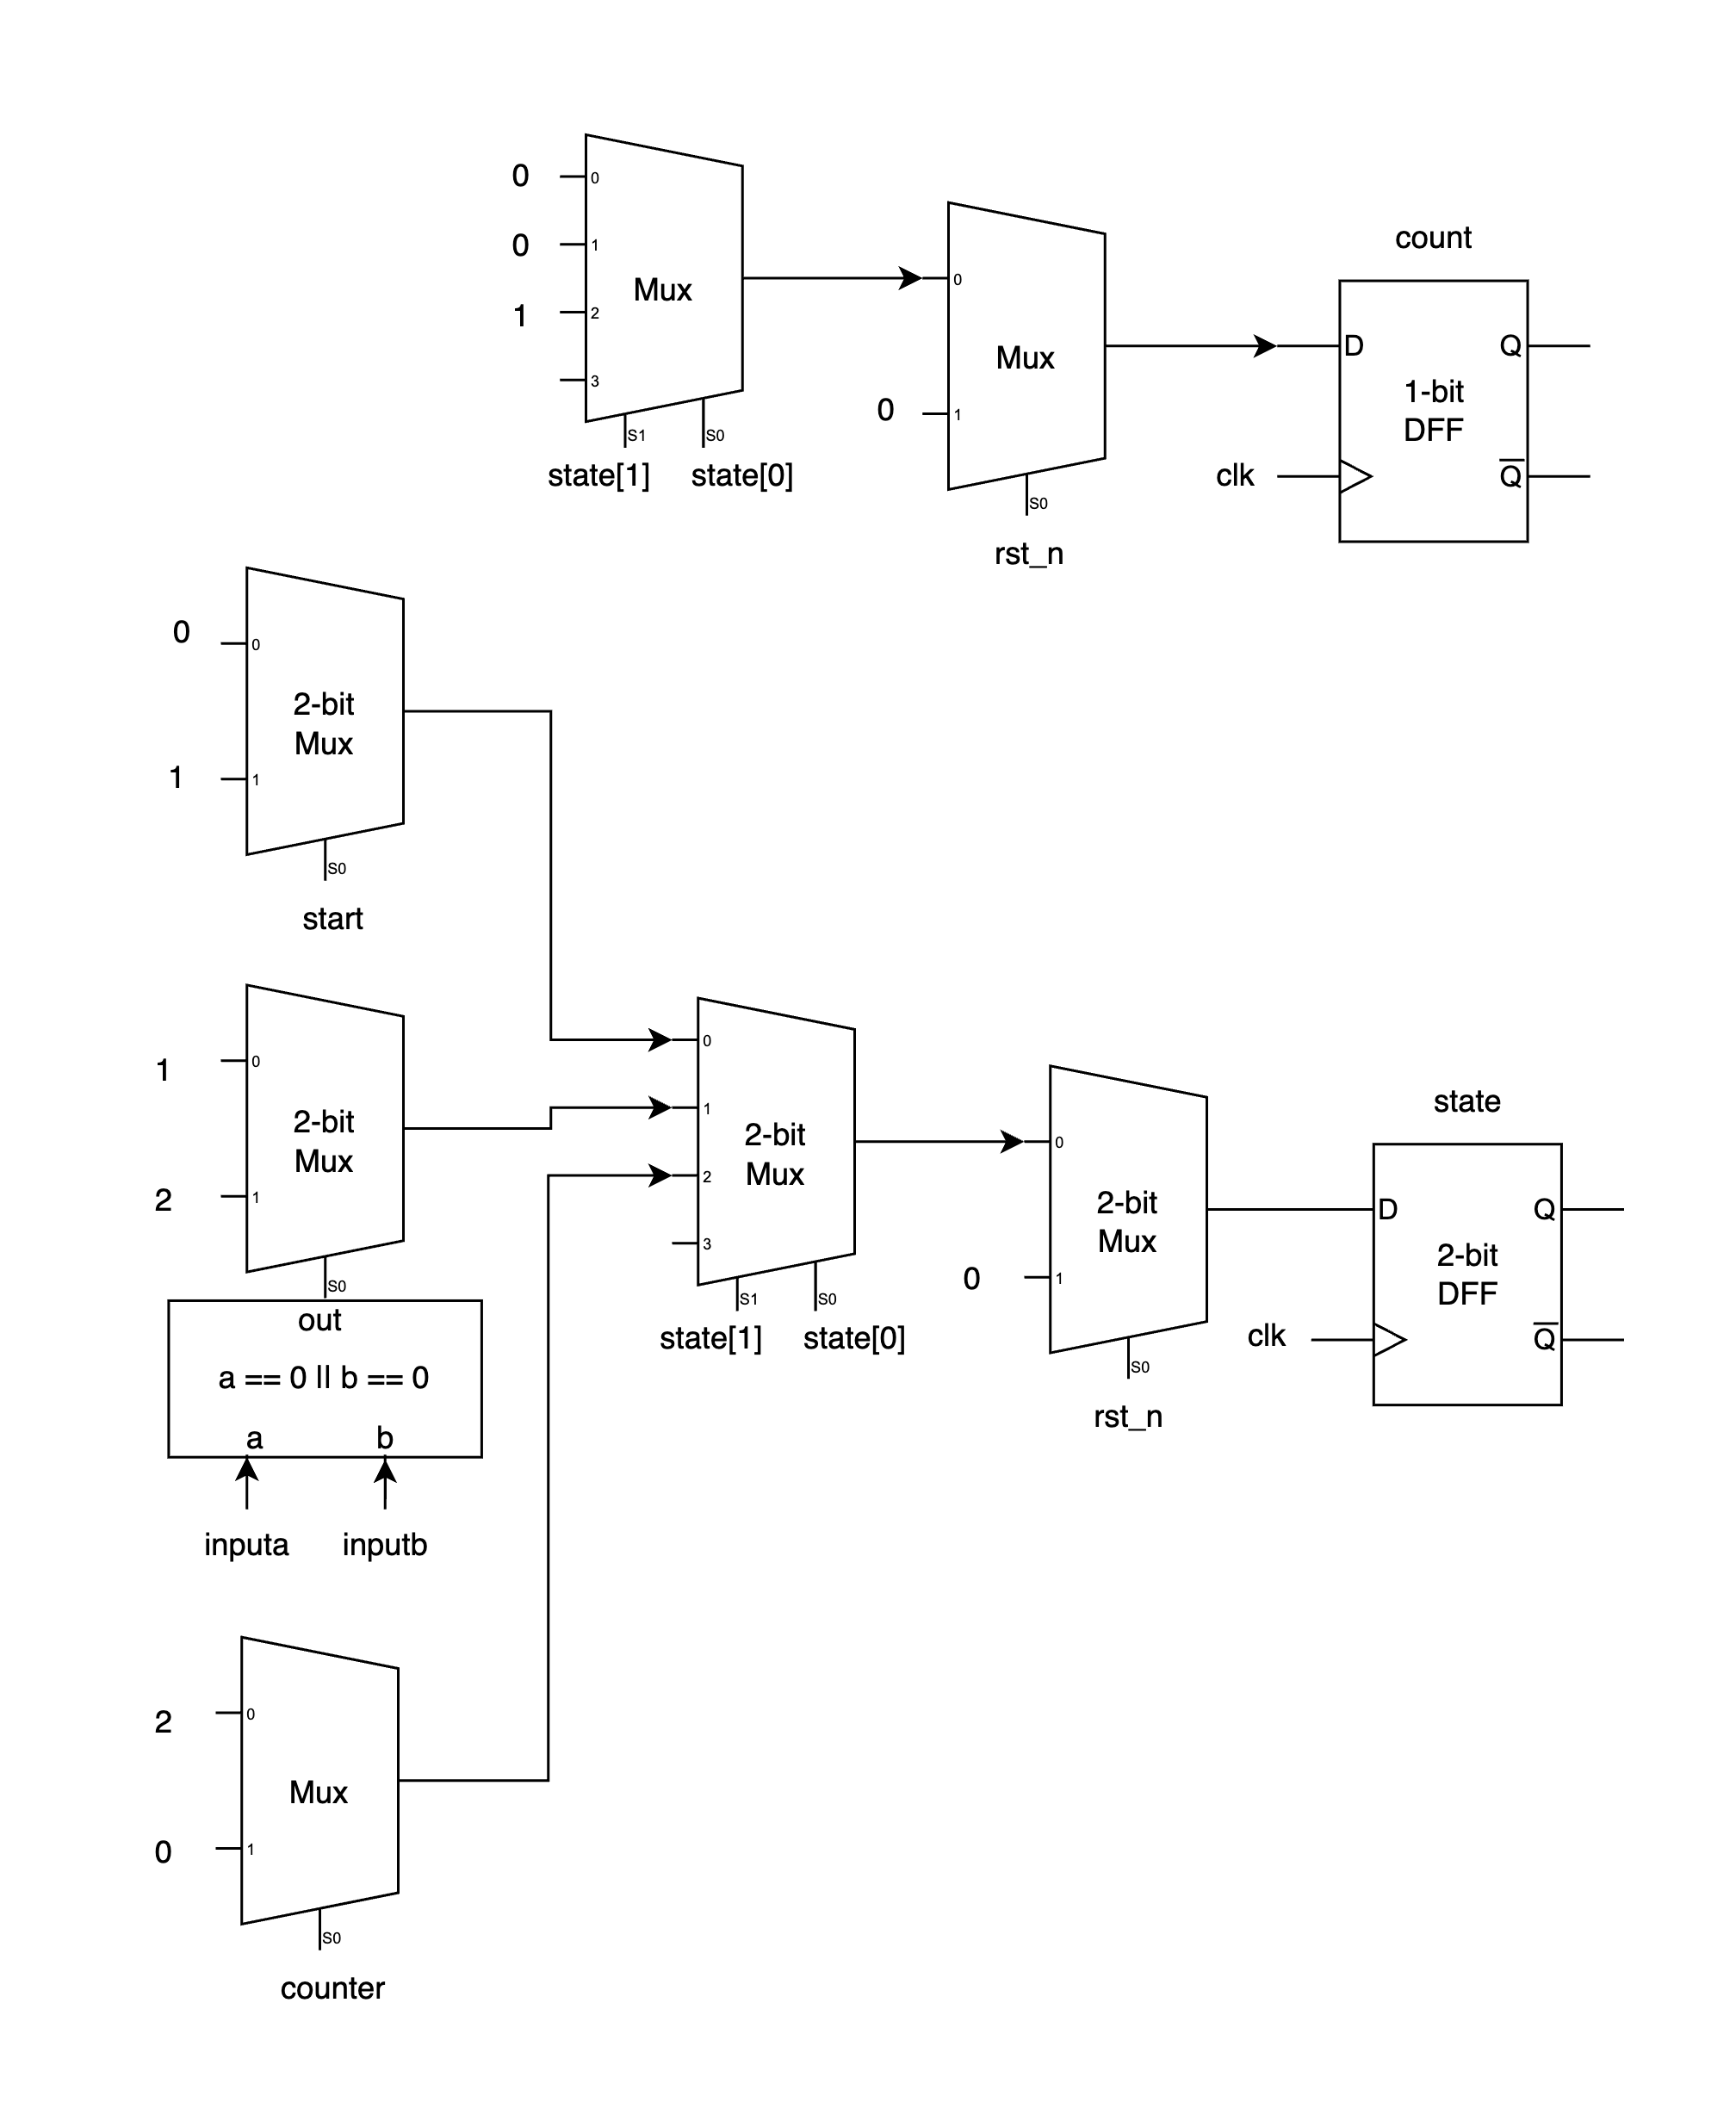
\includegraphics[width=0.8\textwidth]{./img/Q3-counter.png}
  \caption{Q3 Counter Circuit}
  \label{fig:Q3-counter}
\end{figure}

\newpage

接著是輾轉相除法的實作:
% TODO: 輾轉相除法的實作
\begin{figure}[h!]
  \centering
  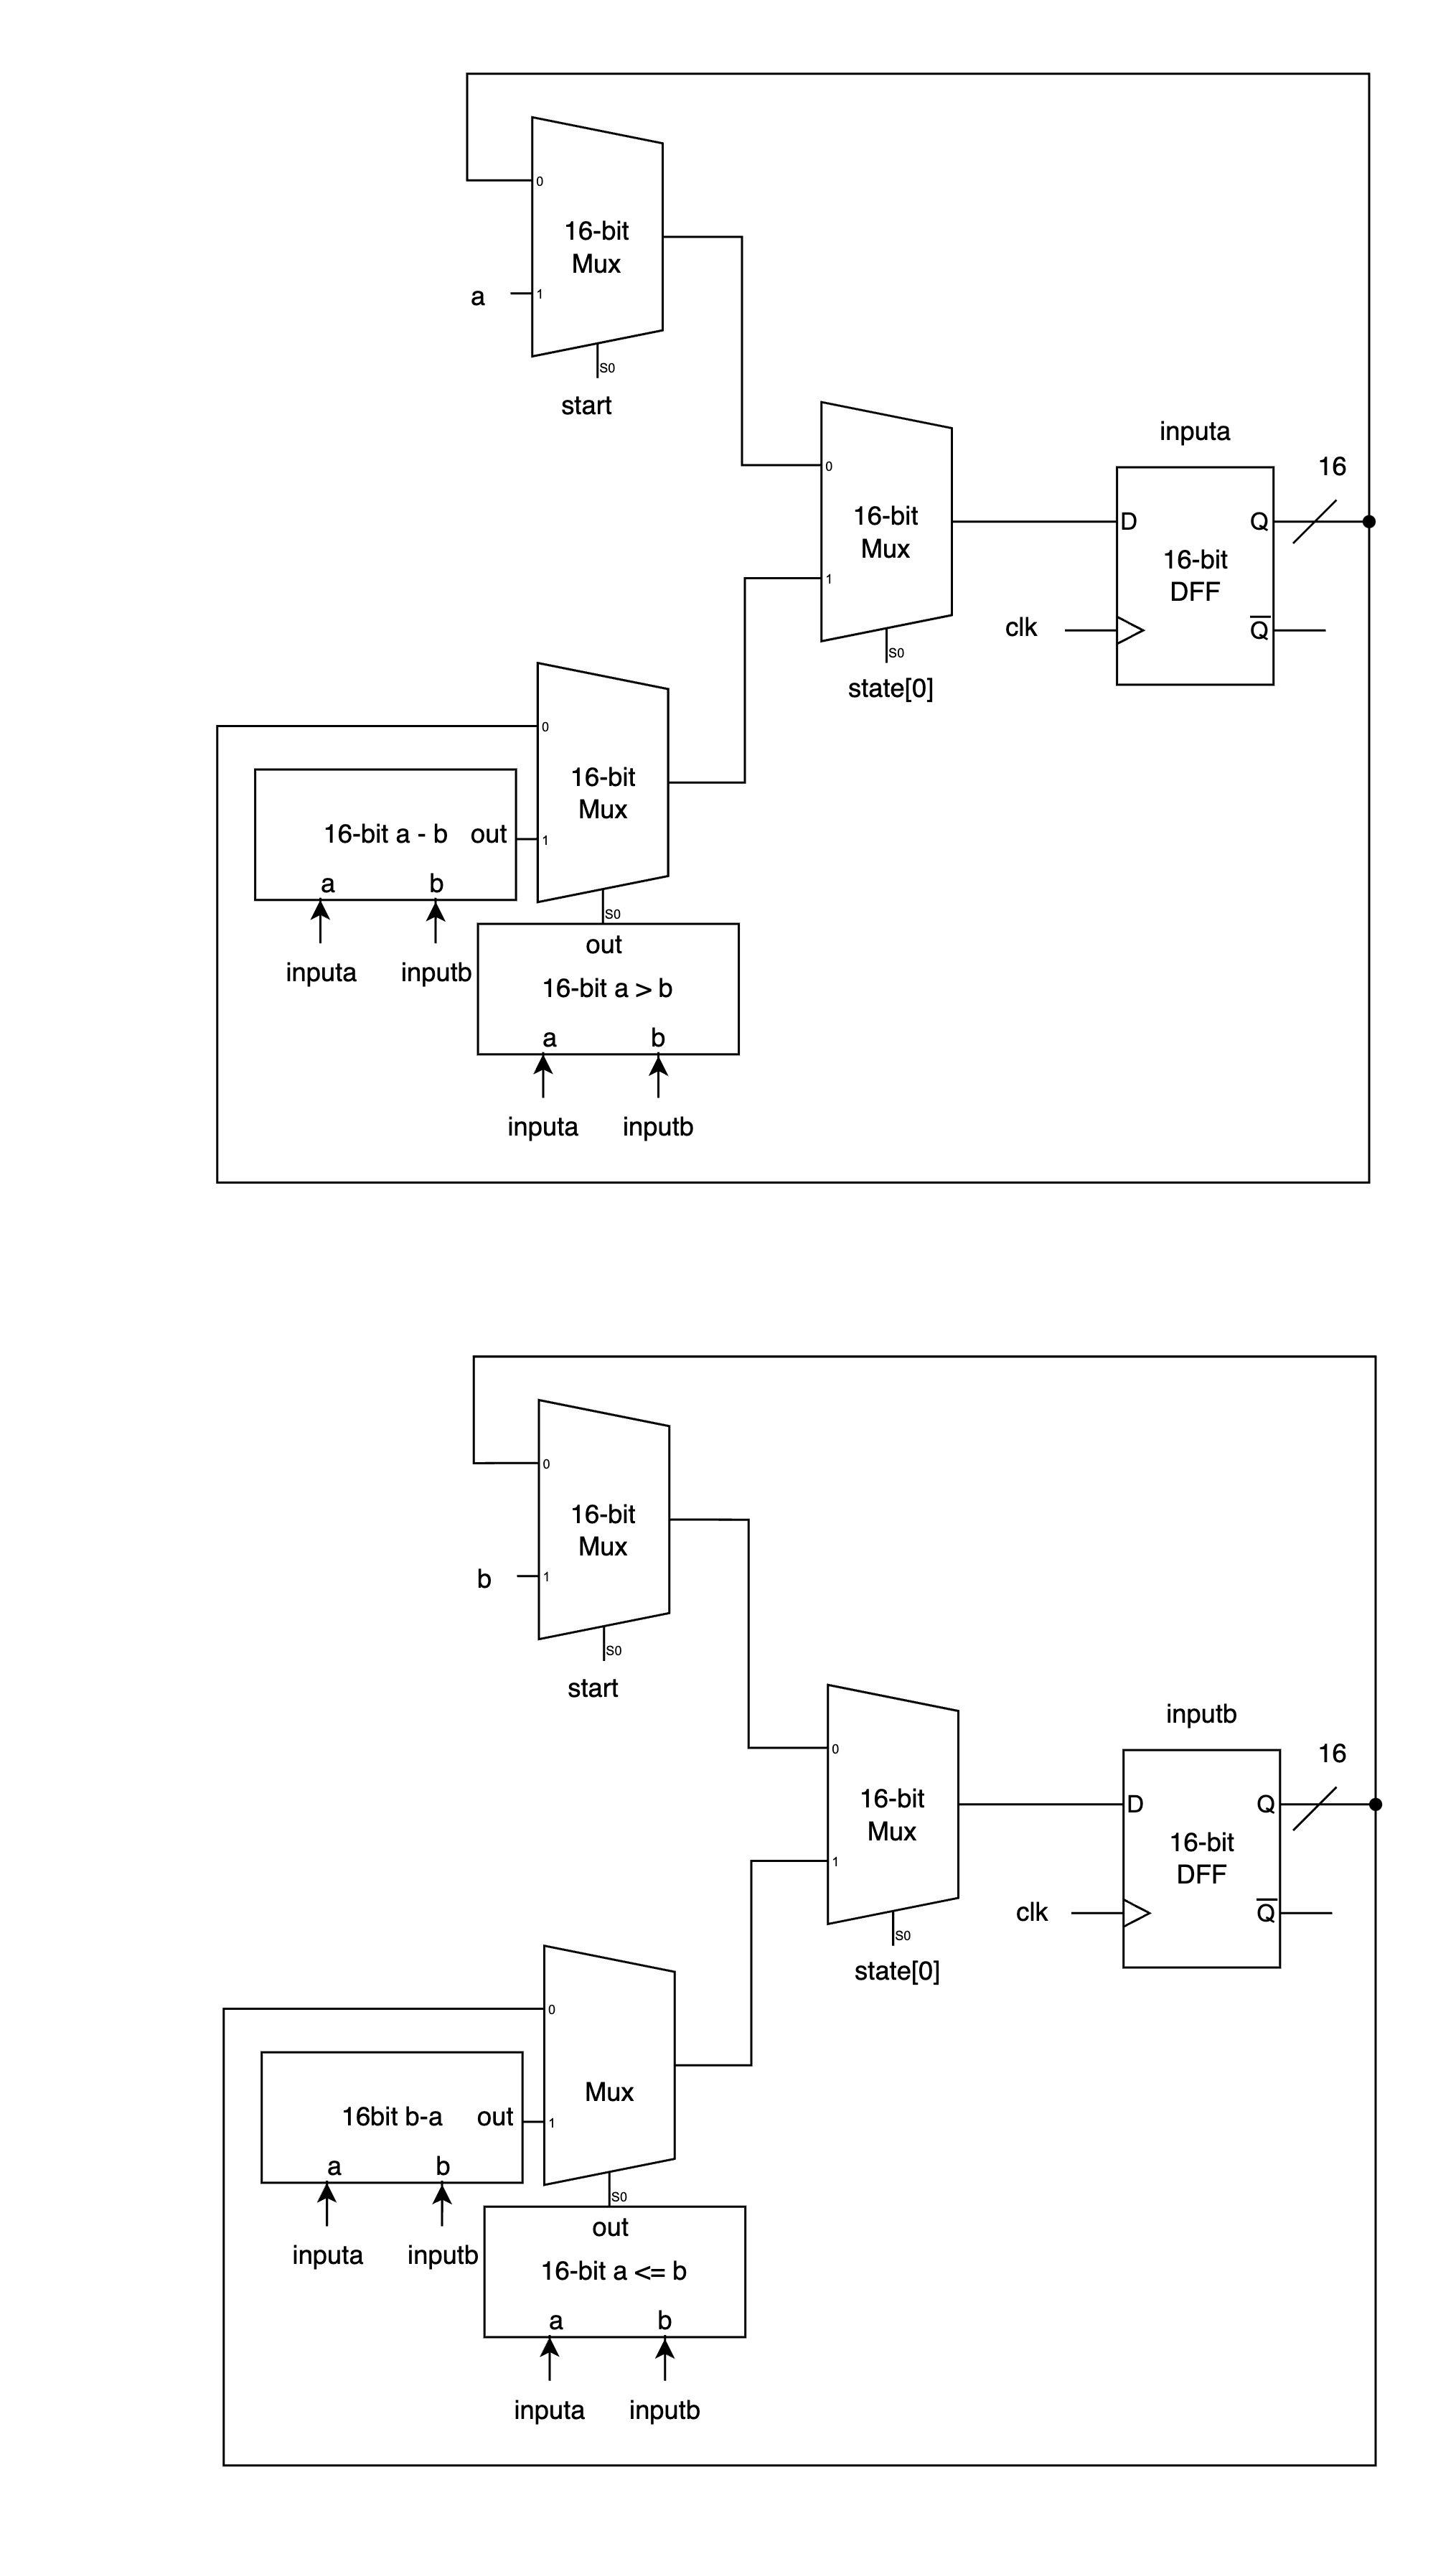
\includegraphics[width=0.7\textwidth]{./img/Q3-ab.png}
  \caption{Q3 Euclidean Circuit}
  \label{fig:Q3-euclidean}
\end{figure}
\newpage
最後是 gcd 與 done 的輸出:
\begin{figure}[h!]
  \centering
  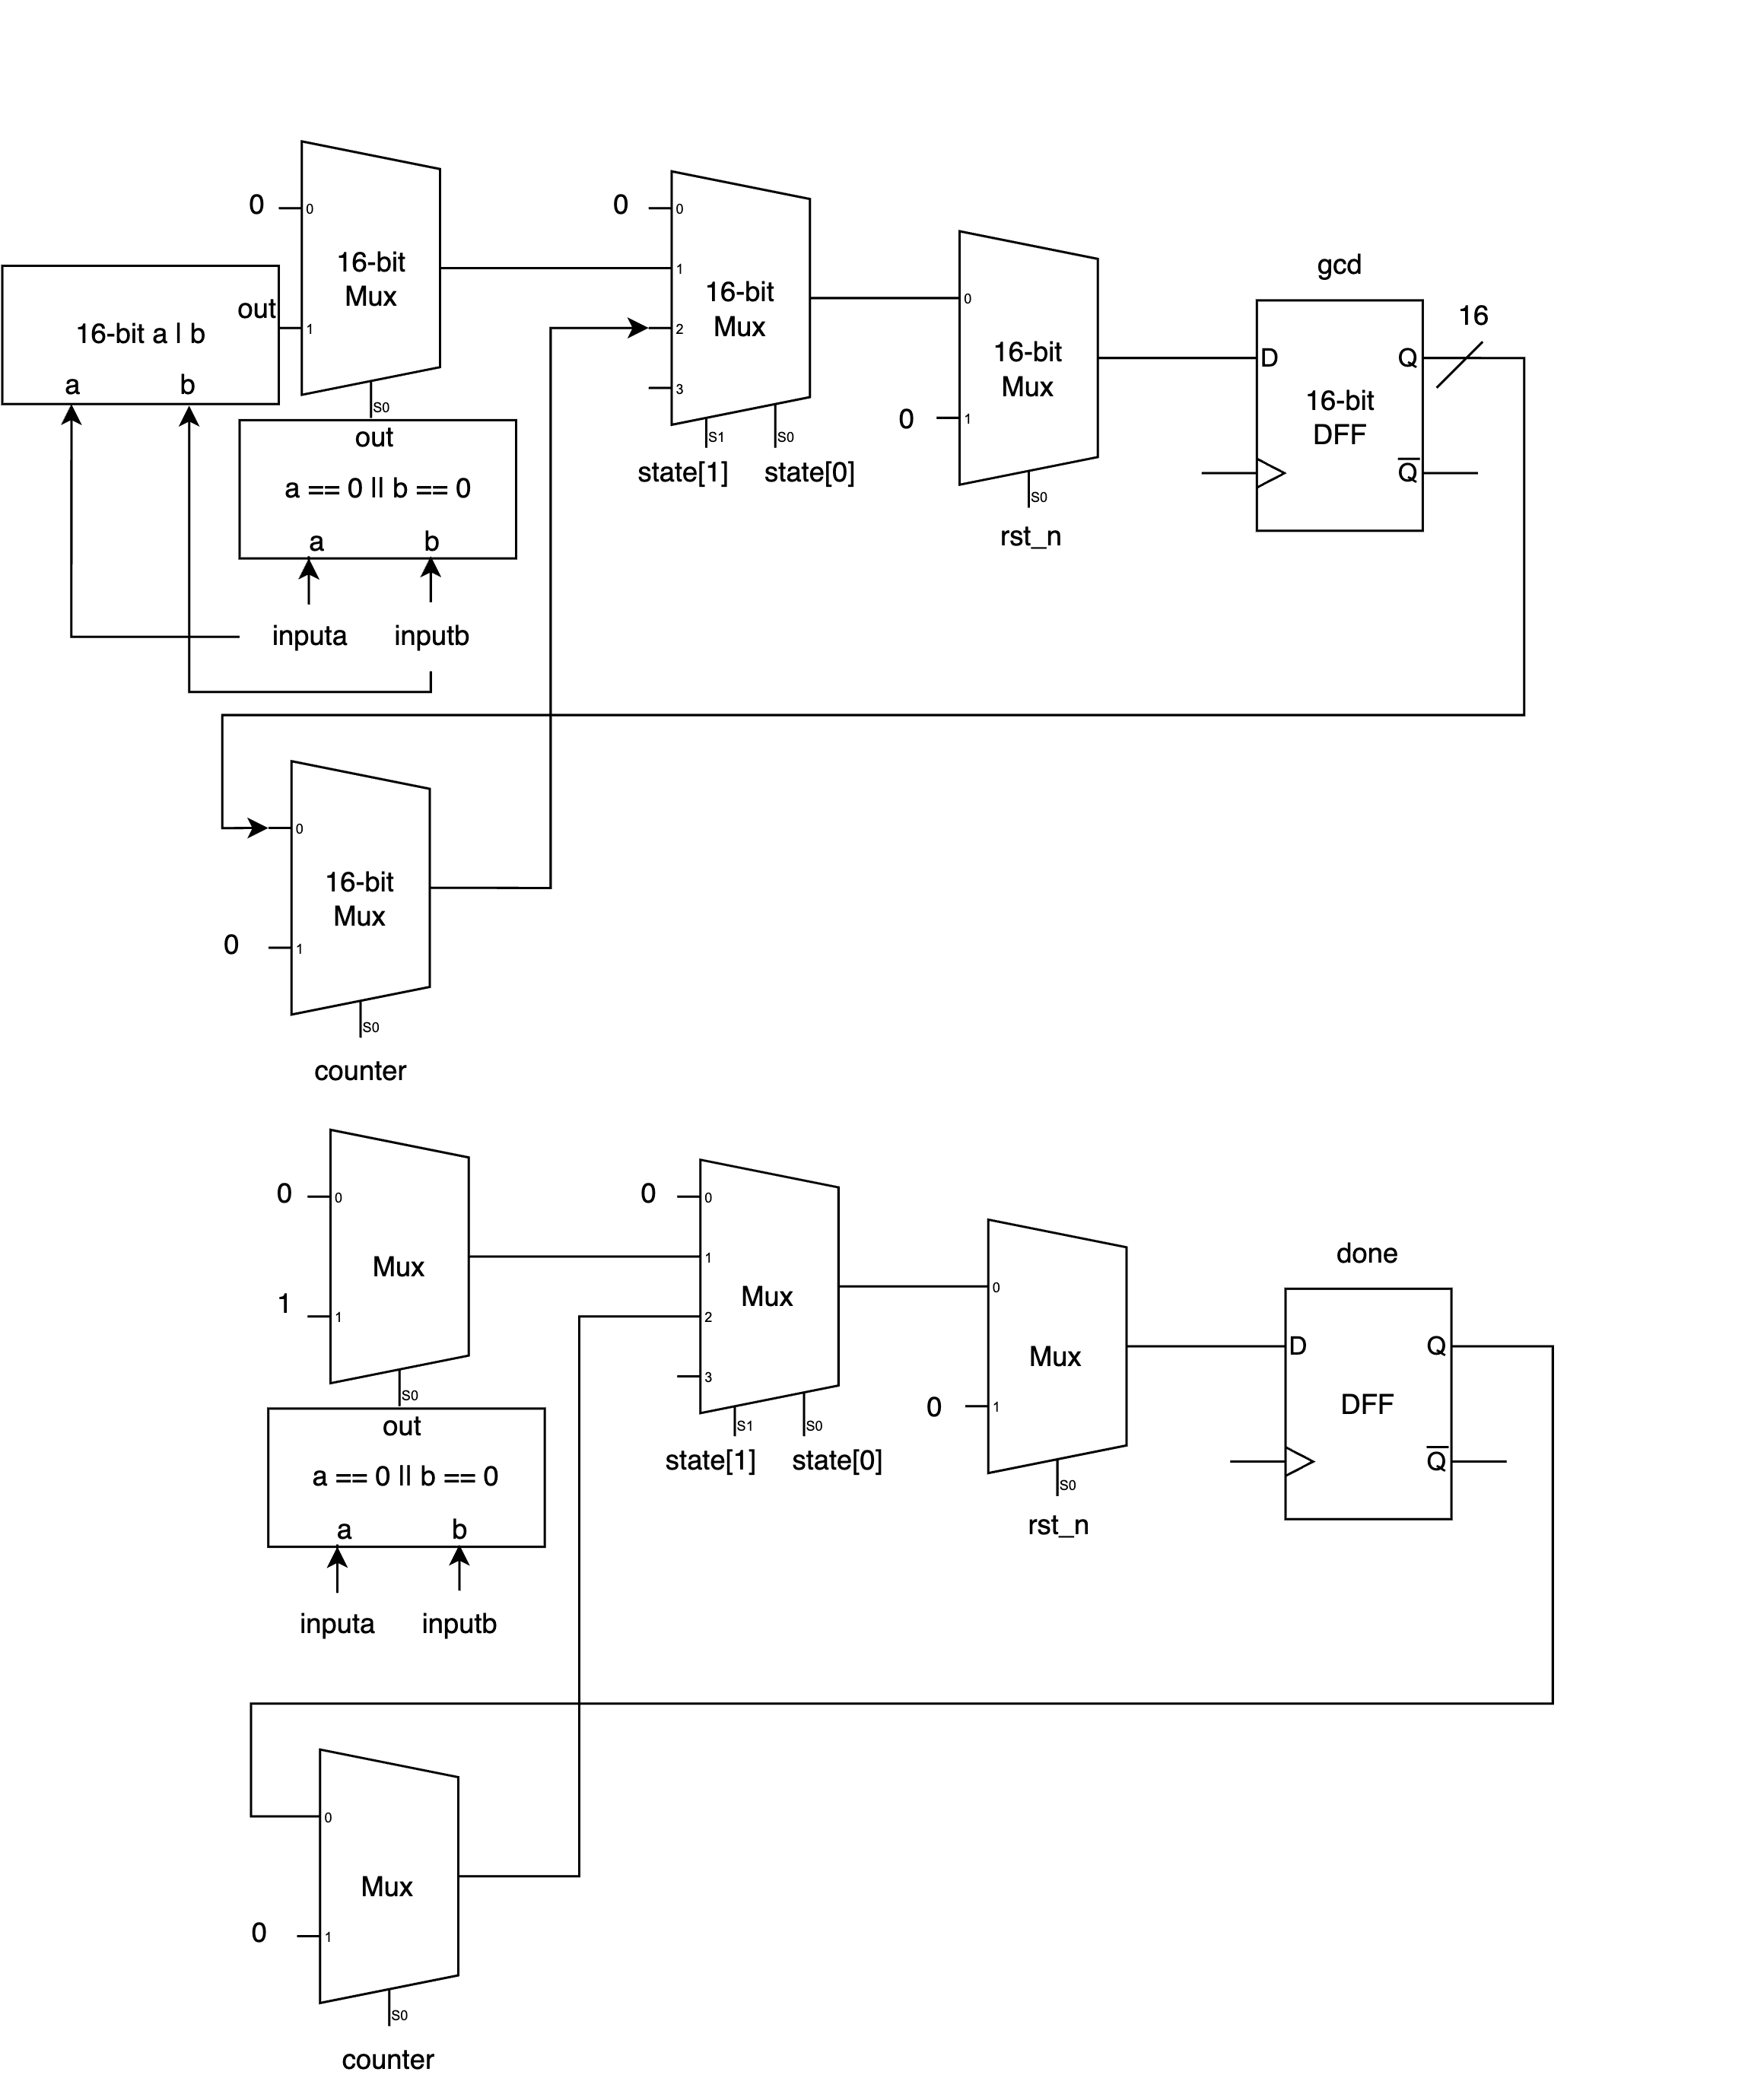
\includegraphics[width=0.7\textwidth]{./img/Q3-gcd.png}
  \caption{Q3 Output}
  \label{fig:Q3-gcd}
\end{figure}
\subsection{Simulation}
我們使用 random 來產生 a, b 的值,並觀察 gcd 的輸出是否正確。

\begin{figure}[h!]
  \centering
  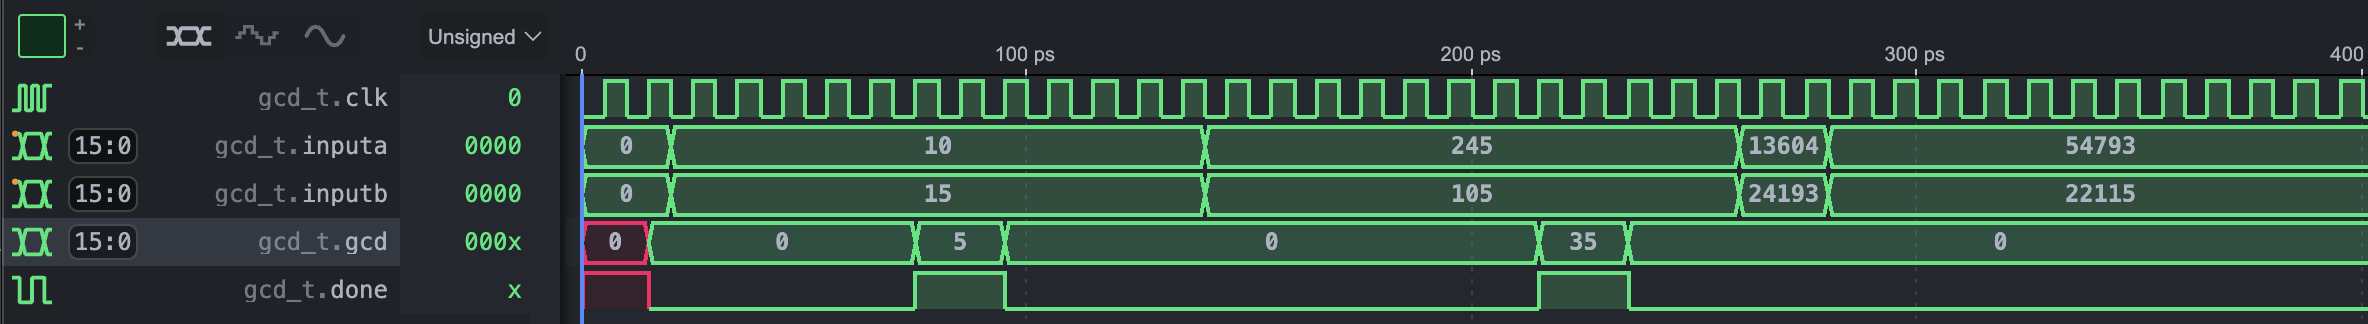
\includegraphics[width=0.8\textwidth]{./img/Q3-tb.png}
  \caption{Q3 Waveform}
  \label{fig:Q3-waveform}
\end{figure}

\newpage

\section{FPGA1: Mixed keyboard and audio modules together}

這題要在 FPGA 上實作一個播放 C4 ~ C8 音階的功能,當按下 w 鍵時,音調會往上播放、按下 s 鍵時,音調會往下播放、\
按下 r 鍵時,會在 1 秒與 0.5 秒之間互相切換播放速度。

\subsection{Implementation}

首先是 Decoder 的部分,這邊會接收兩個輸入:tone, height,分別代表音調和音高,\
如 C4 就會被分成 C, 4,並輸出相對應的音調頻率。
\par
以 C 這個音為例,C4 的時候頻率就是 262 Hz,C5 的時候就是 $262 \times 2^1$,C6 則是 $262 \times 2^2$,以此類推,\
因此我直接使用 left shift 音高減掉四位元,就能夠得到相對應的頻率。

\begin{figure}[h!]
  \centering
  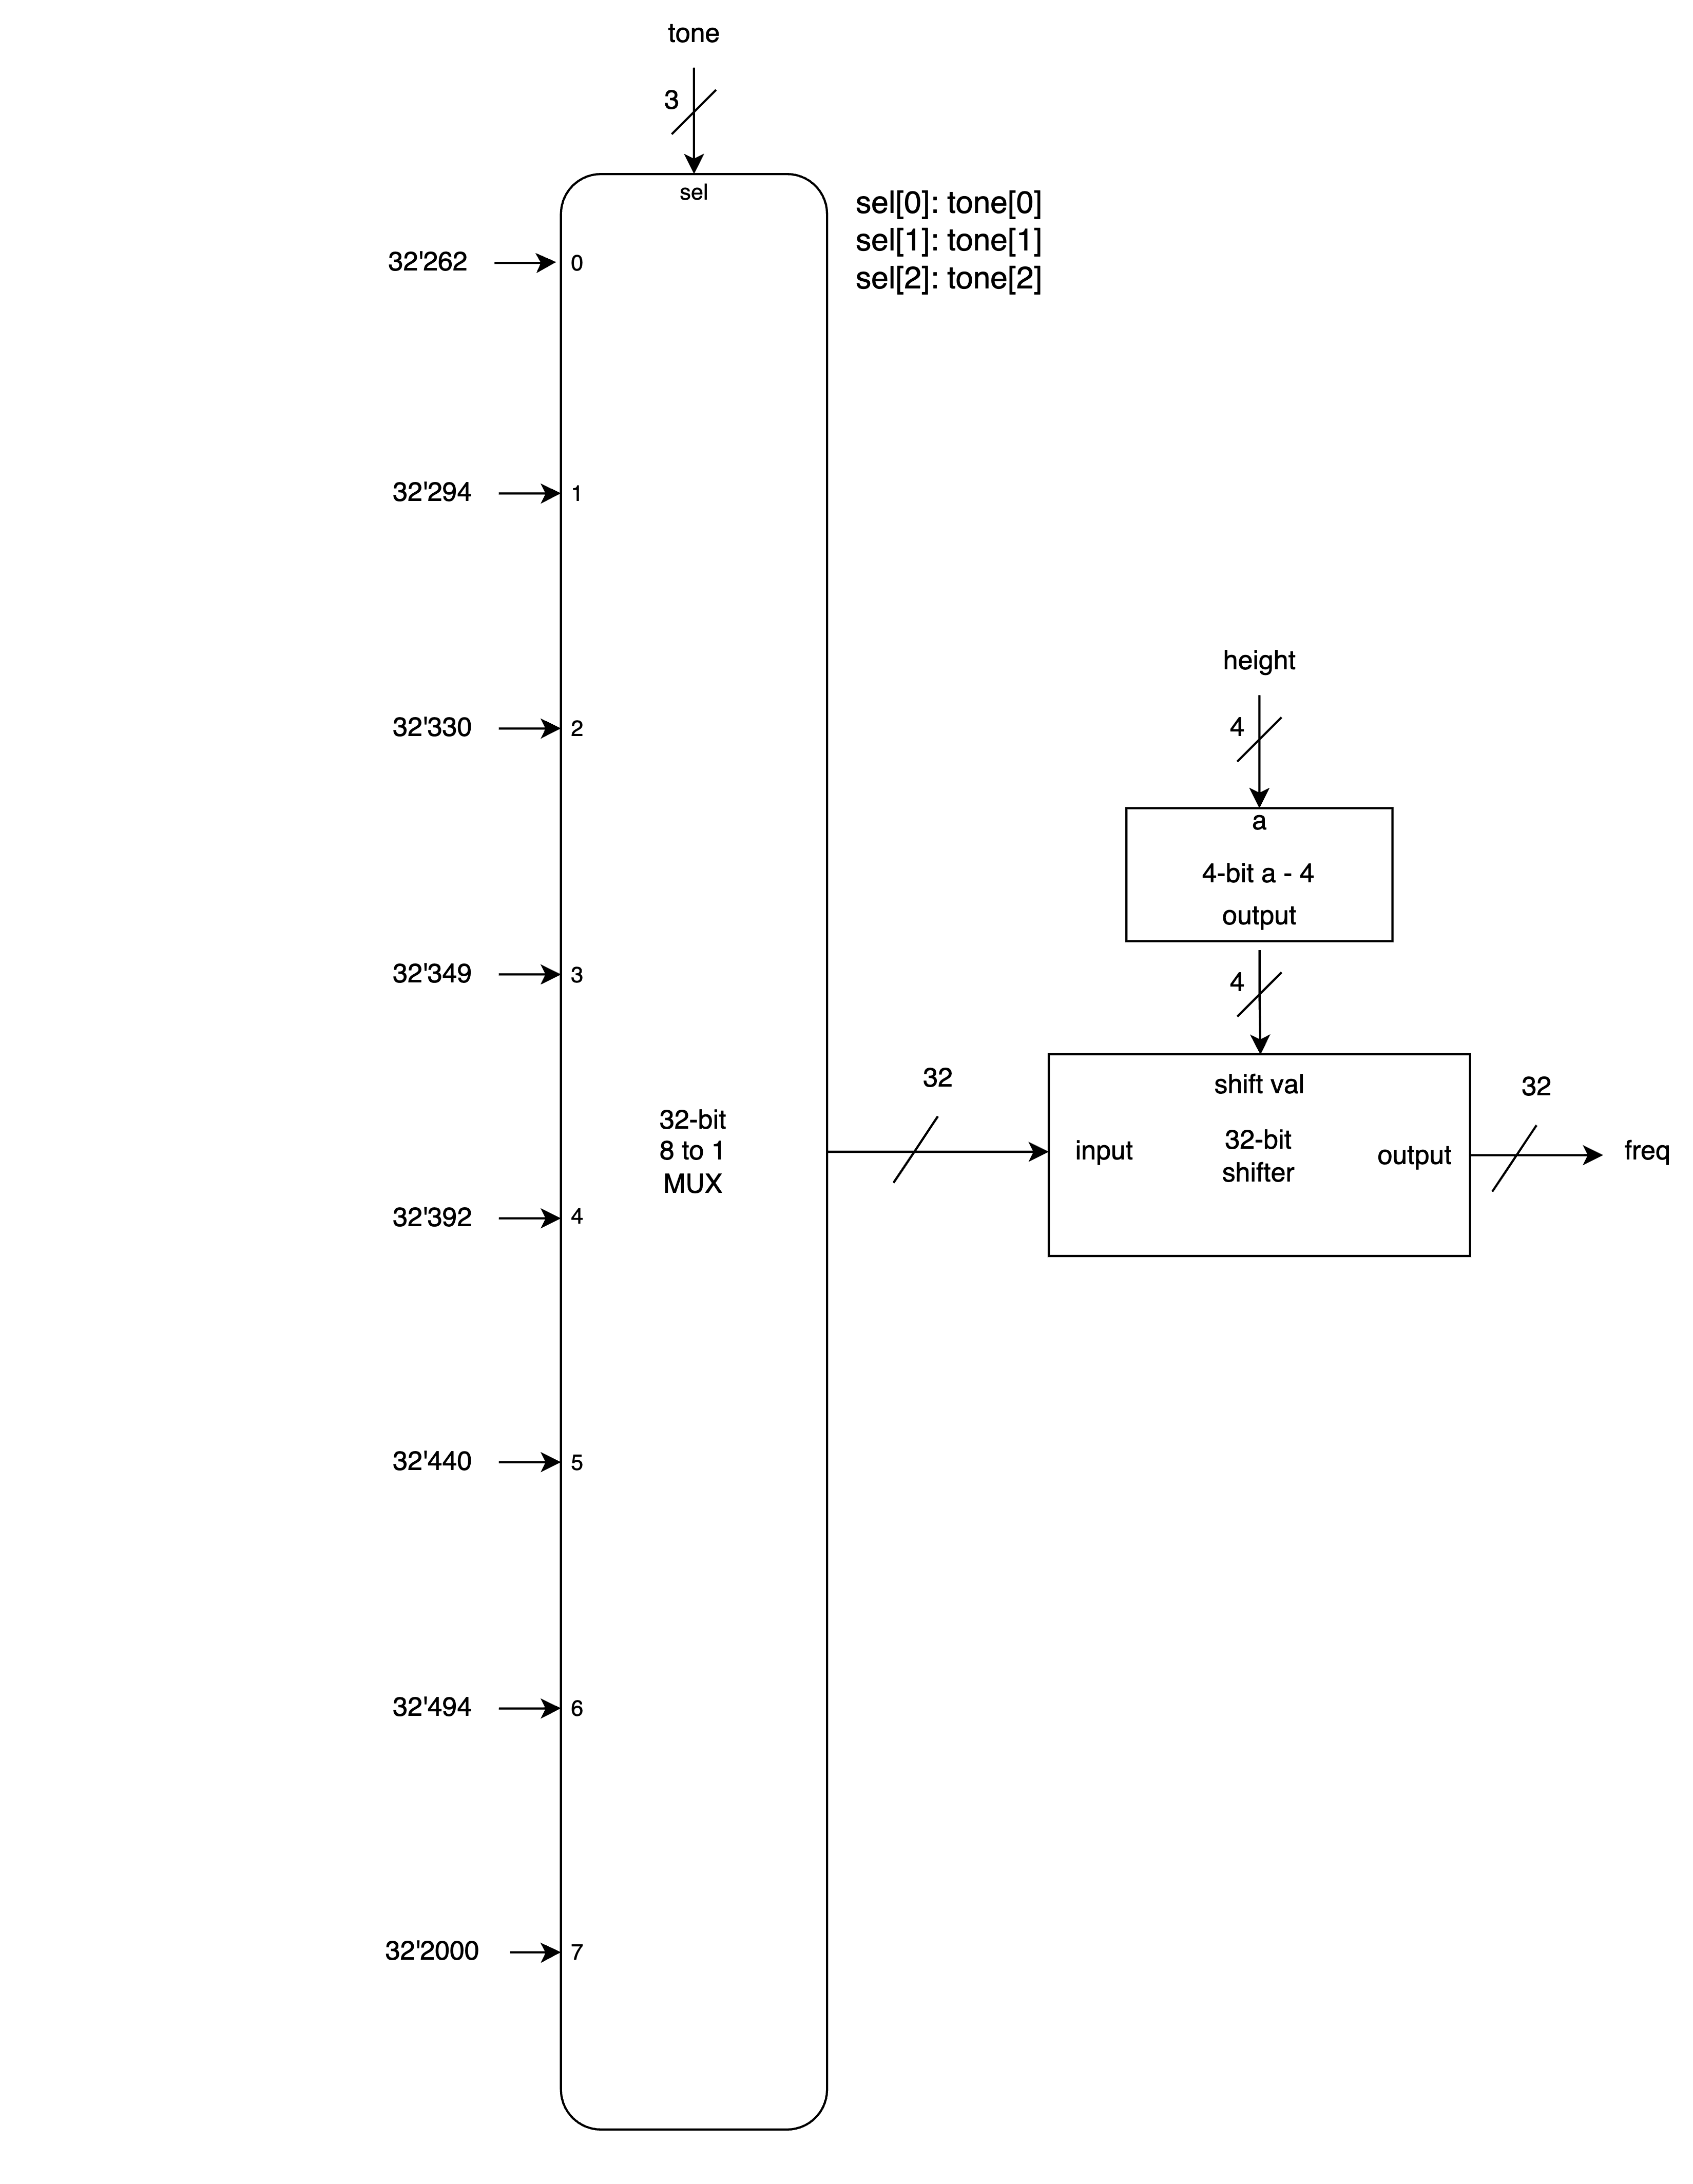
\includegraphics[width=0.7\textwidth]{./img/FPGA1-decoder.png}
  \caption{FPGA1 Decoder}
  \label{fig:FPGA1-decoder}
\end{figure}
\newpage

接著是音階控制的部分,首先是速度,fast = 0 時代表每一秒更新,fast = 1 時代表每半秒更新。當按下鍵盤 R 時,
fast 值就會做一次 not 反轉,下圖是這部分的電路圖:

\begin{figure}[h!]
  \centering
  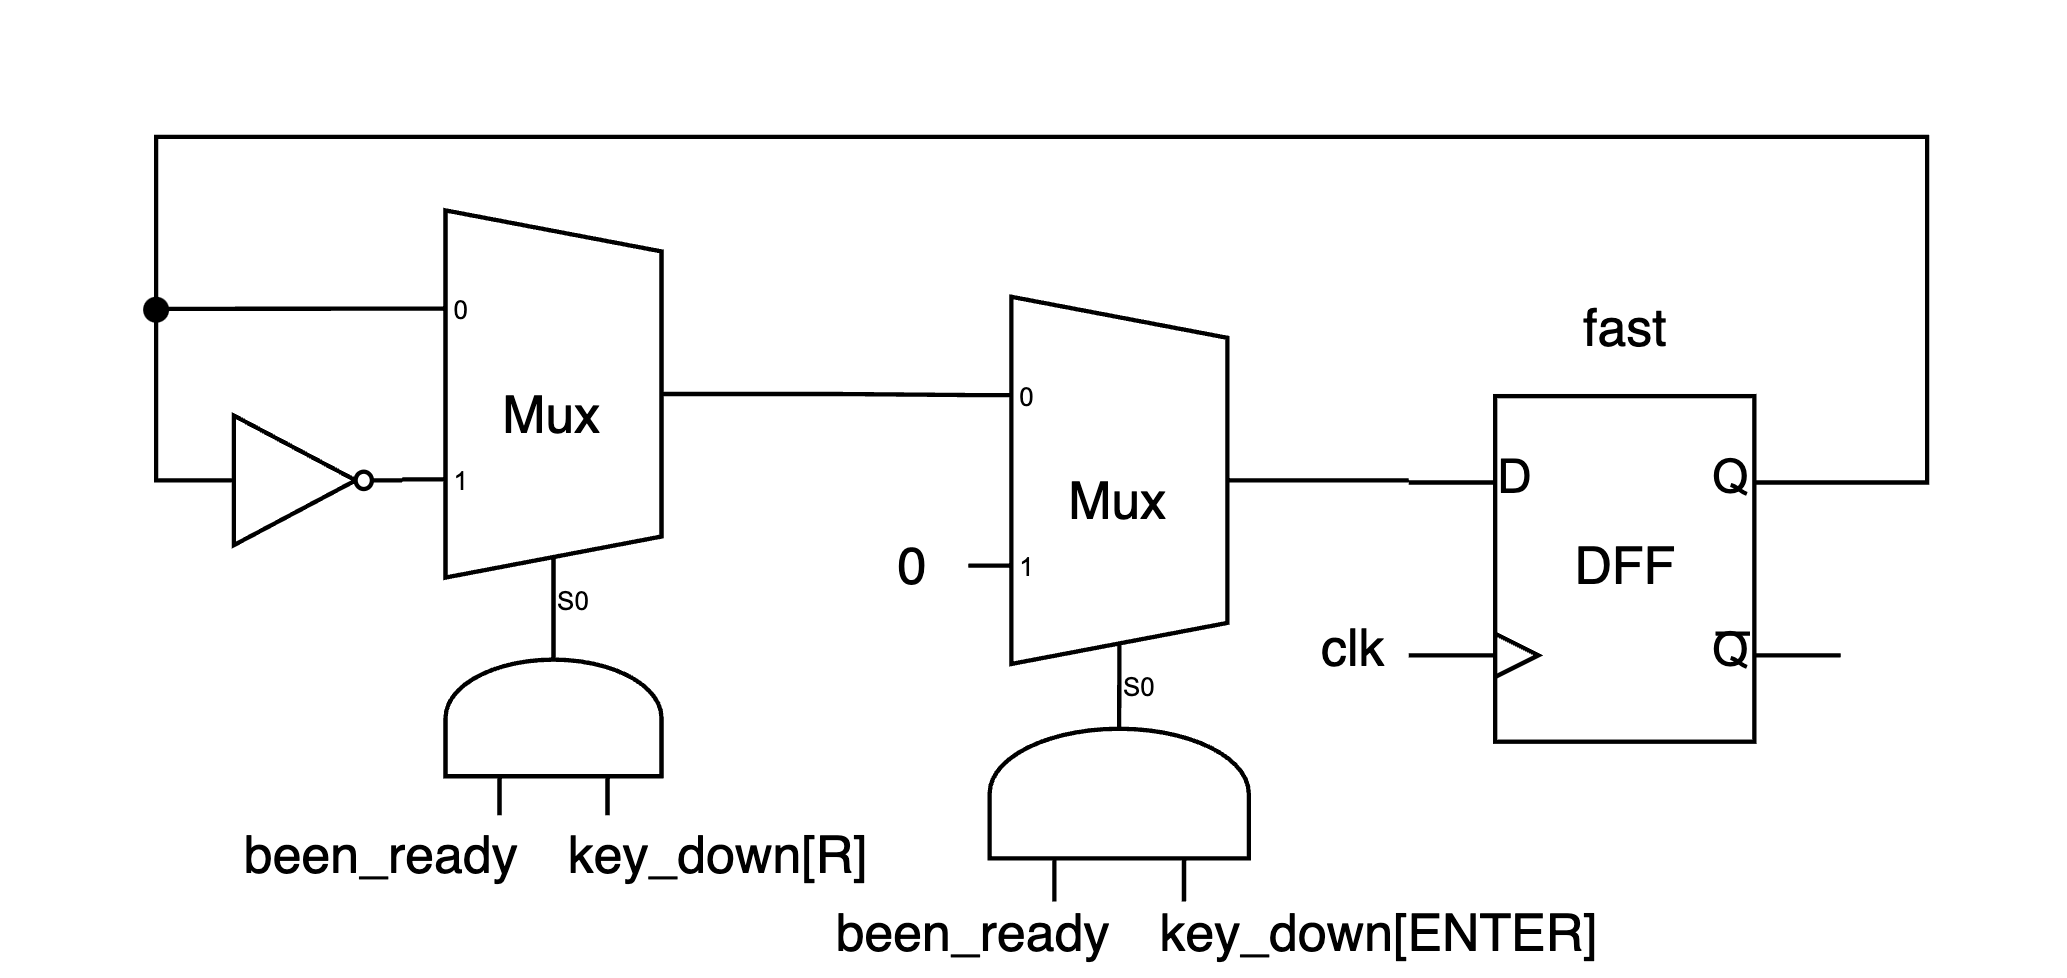
\includegraphics[width=0.8\textwidth]{./img/FPGA1-fast.png}
  \caption{FPGA1 Fast}
  \label{fig:FPGA1-fast}
\end{figure}

接著是 direction,與 fast 的實作方法類似,direction = 0 代表下行,反之則是上行。
實作的部分是改成按下 S 時將 direction 設為 0,按下 W 時將 direction 設為 1。

\begin{figure}[h!]
  \centering
  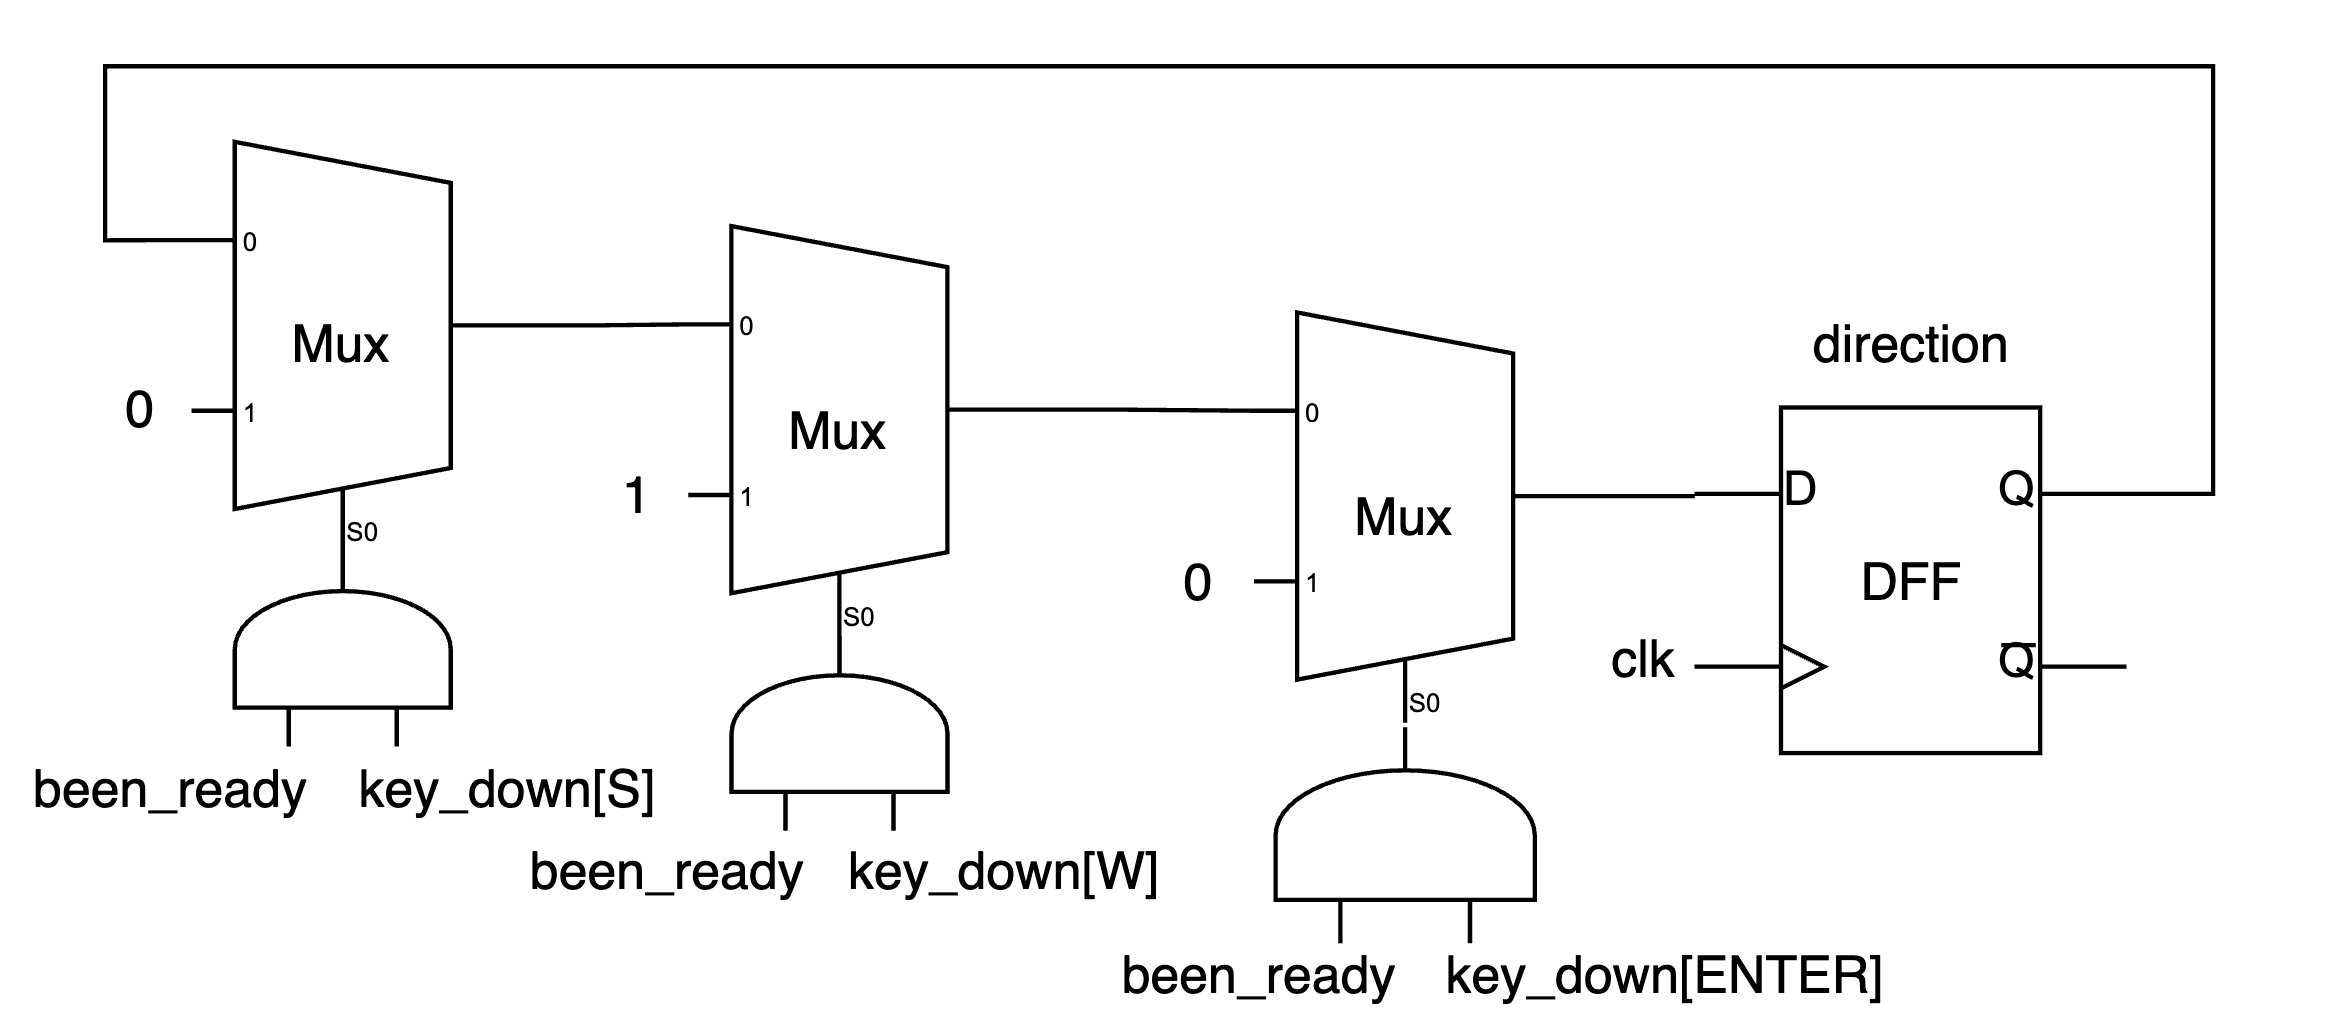
\includegraphics[width=0.8\textwidth]{./img/FPGA1-direction.png}
  \caption{FPGA1 Direction}
  \label{fig:FPGA1-direction}
\end{figure}

\newpage

接下來是 counter,每一個 clock cycle 就會加一,並且根據 fast 的值,輸出一個訊號代表音調是否要更新。

\begin{figure}[h!]
  \centering
  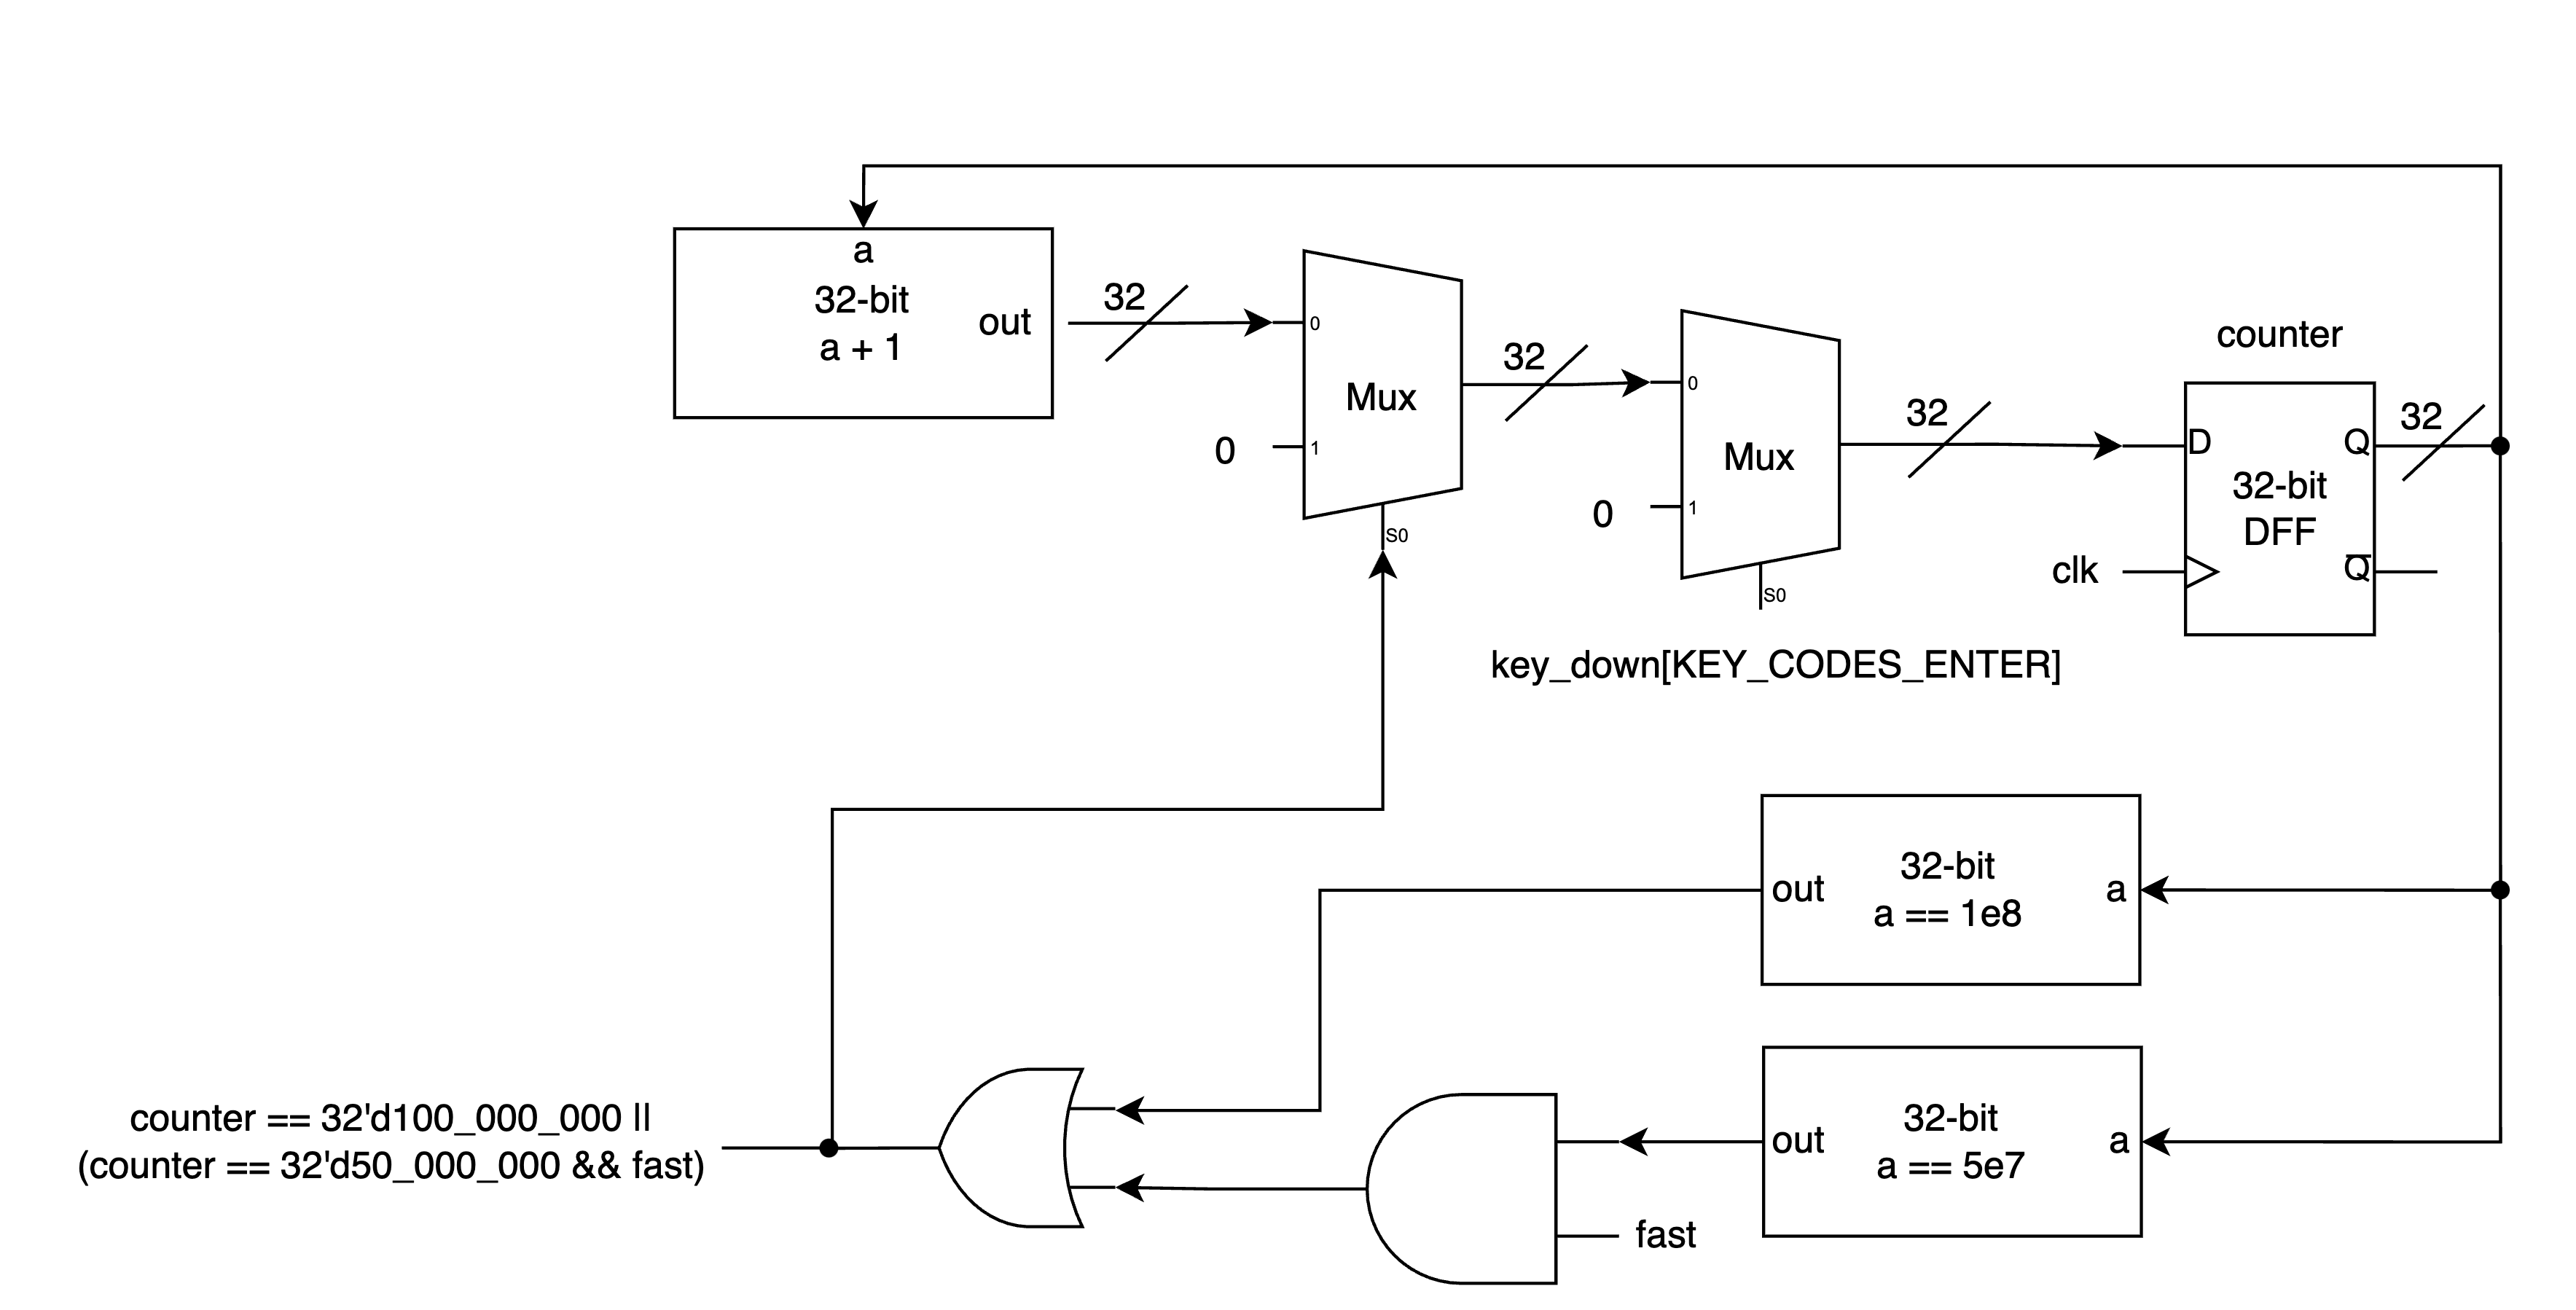
\includegraphics[width=0.8\textwidth]{./img/FPGA1-counter.png}
  \caption{FPGA1 Counter}
  \label{fig:FPGA1-counter}
\end{figure}

有了以上三個 register 後,就可以來實作音調的控制了。首先是 tone 的部分,當音調不在 C4 或 C8 時,\
每次更新就會根據 direction ,將 tone 在 $0 \sim 6$ 的區間加上一或減去一。如果判定會超出範圍就會保持原樣。

\begin{figure}[h!]
  \centering
  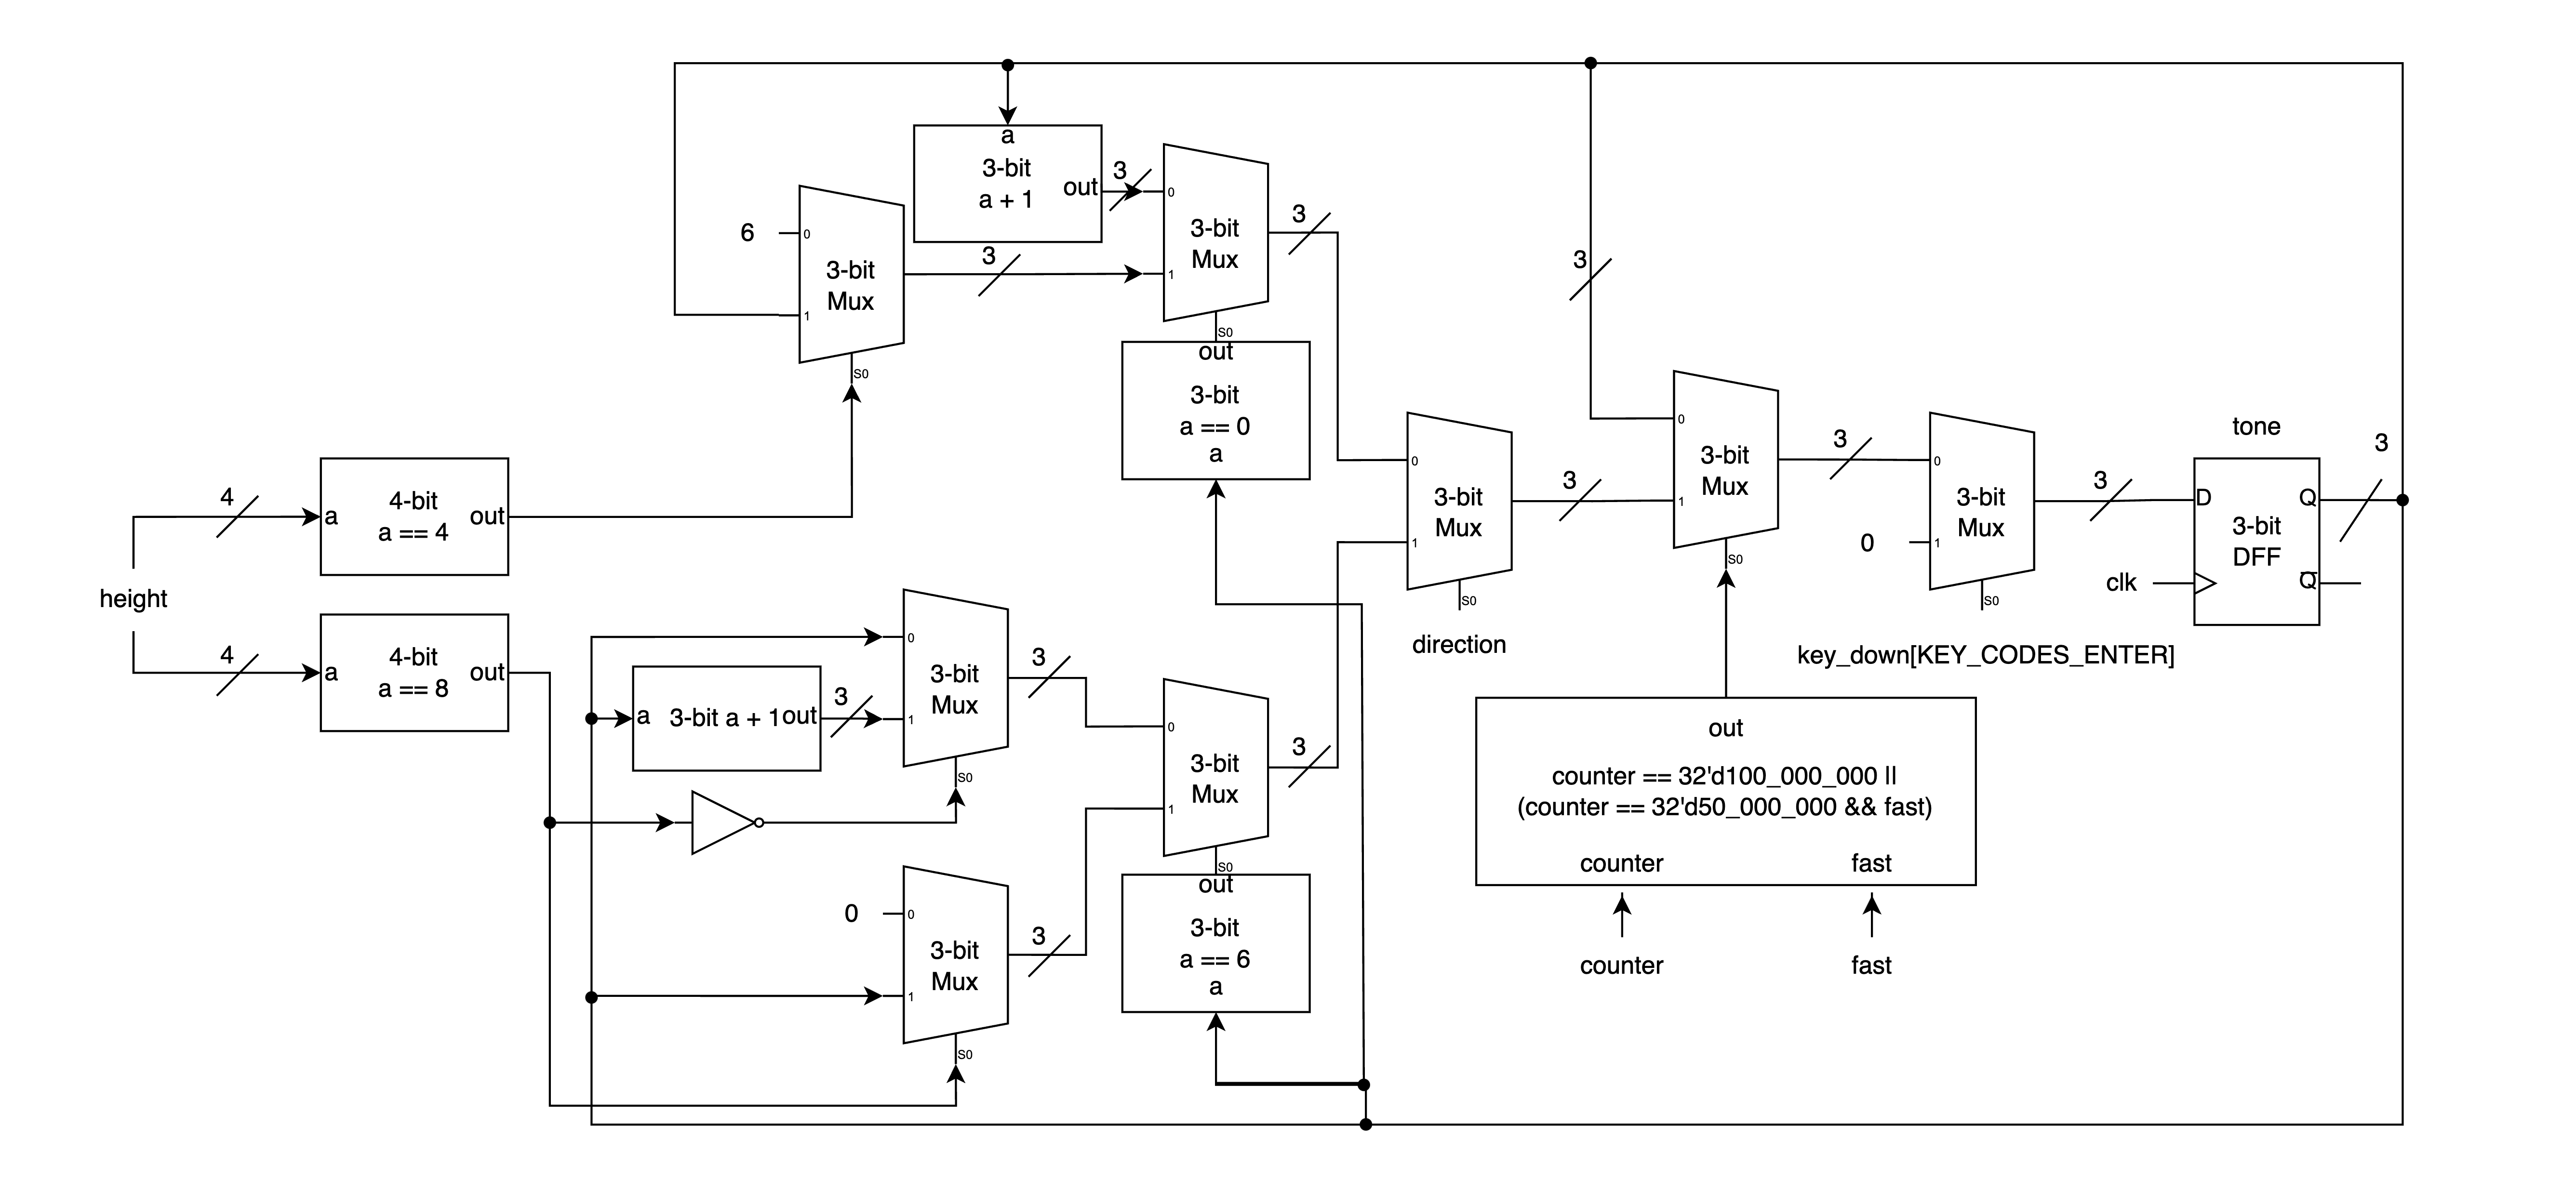
\includegraphics[width=0.7\textwidth]{./img/FPGA1-tone.png}
  \caption{FPGA1 Tone}
  \label{fig:FPGA1-tone}
\end{figure}

\newpage

接著是 height,每次更新時會檢測 tone 是否有 overflow 或是 underflow,並根據情況加減一。\
如果判定會超出範圍也會保持原諒。

\begin{figure}[h!]
  \centering
  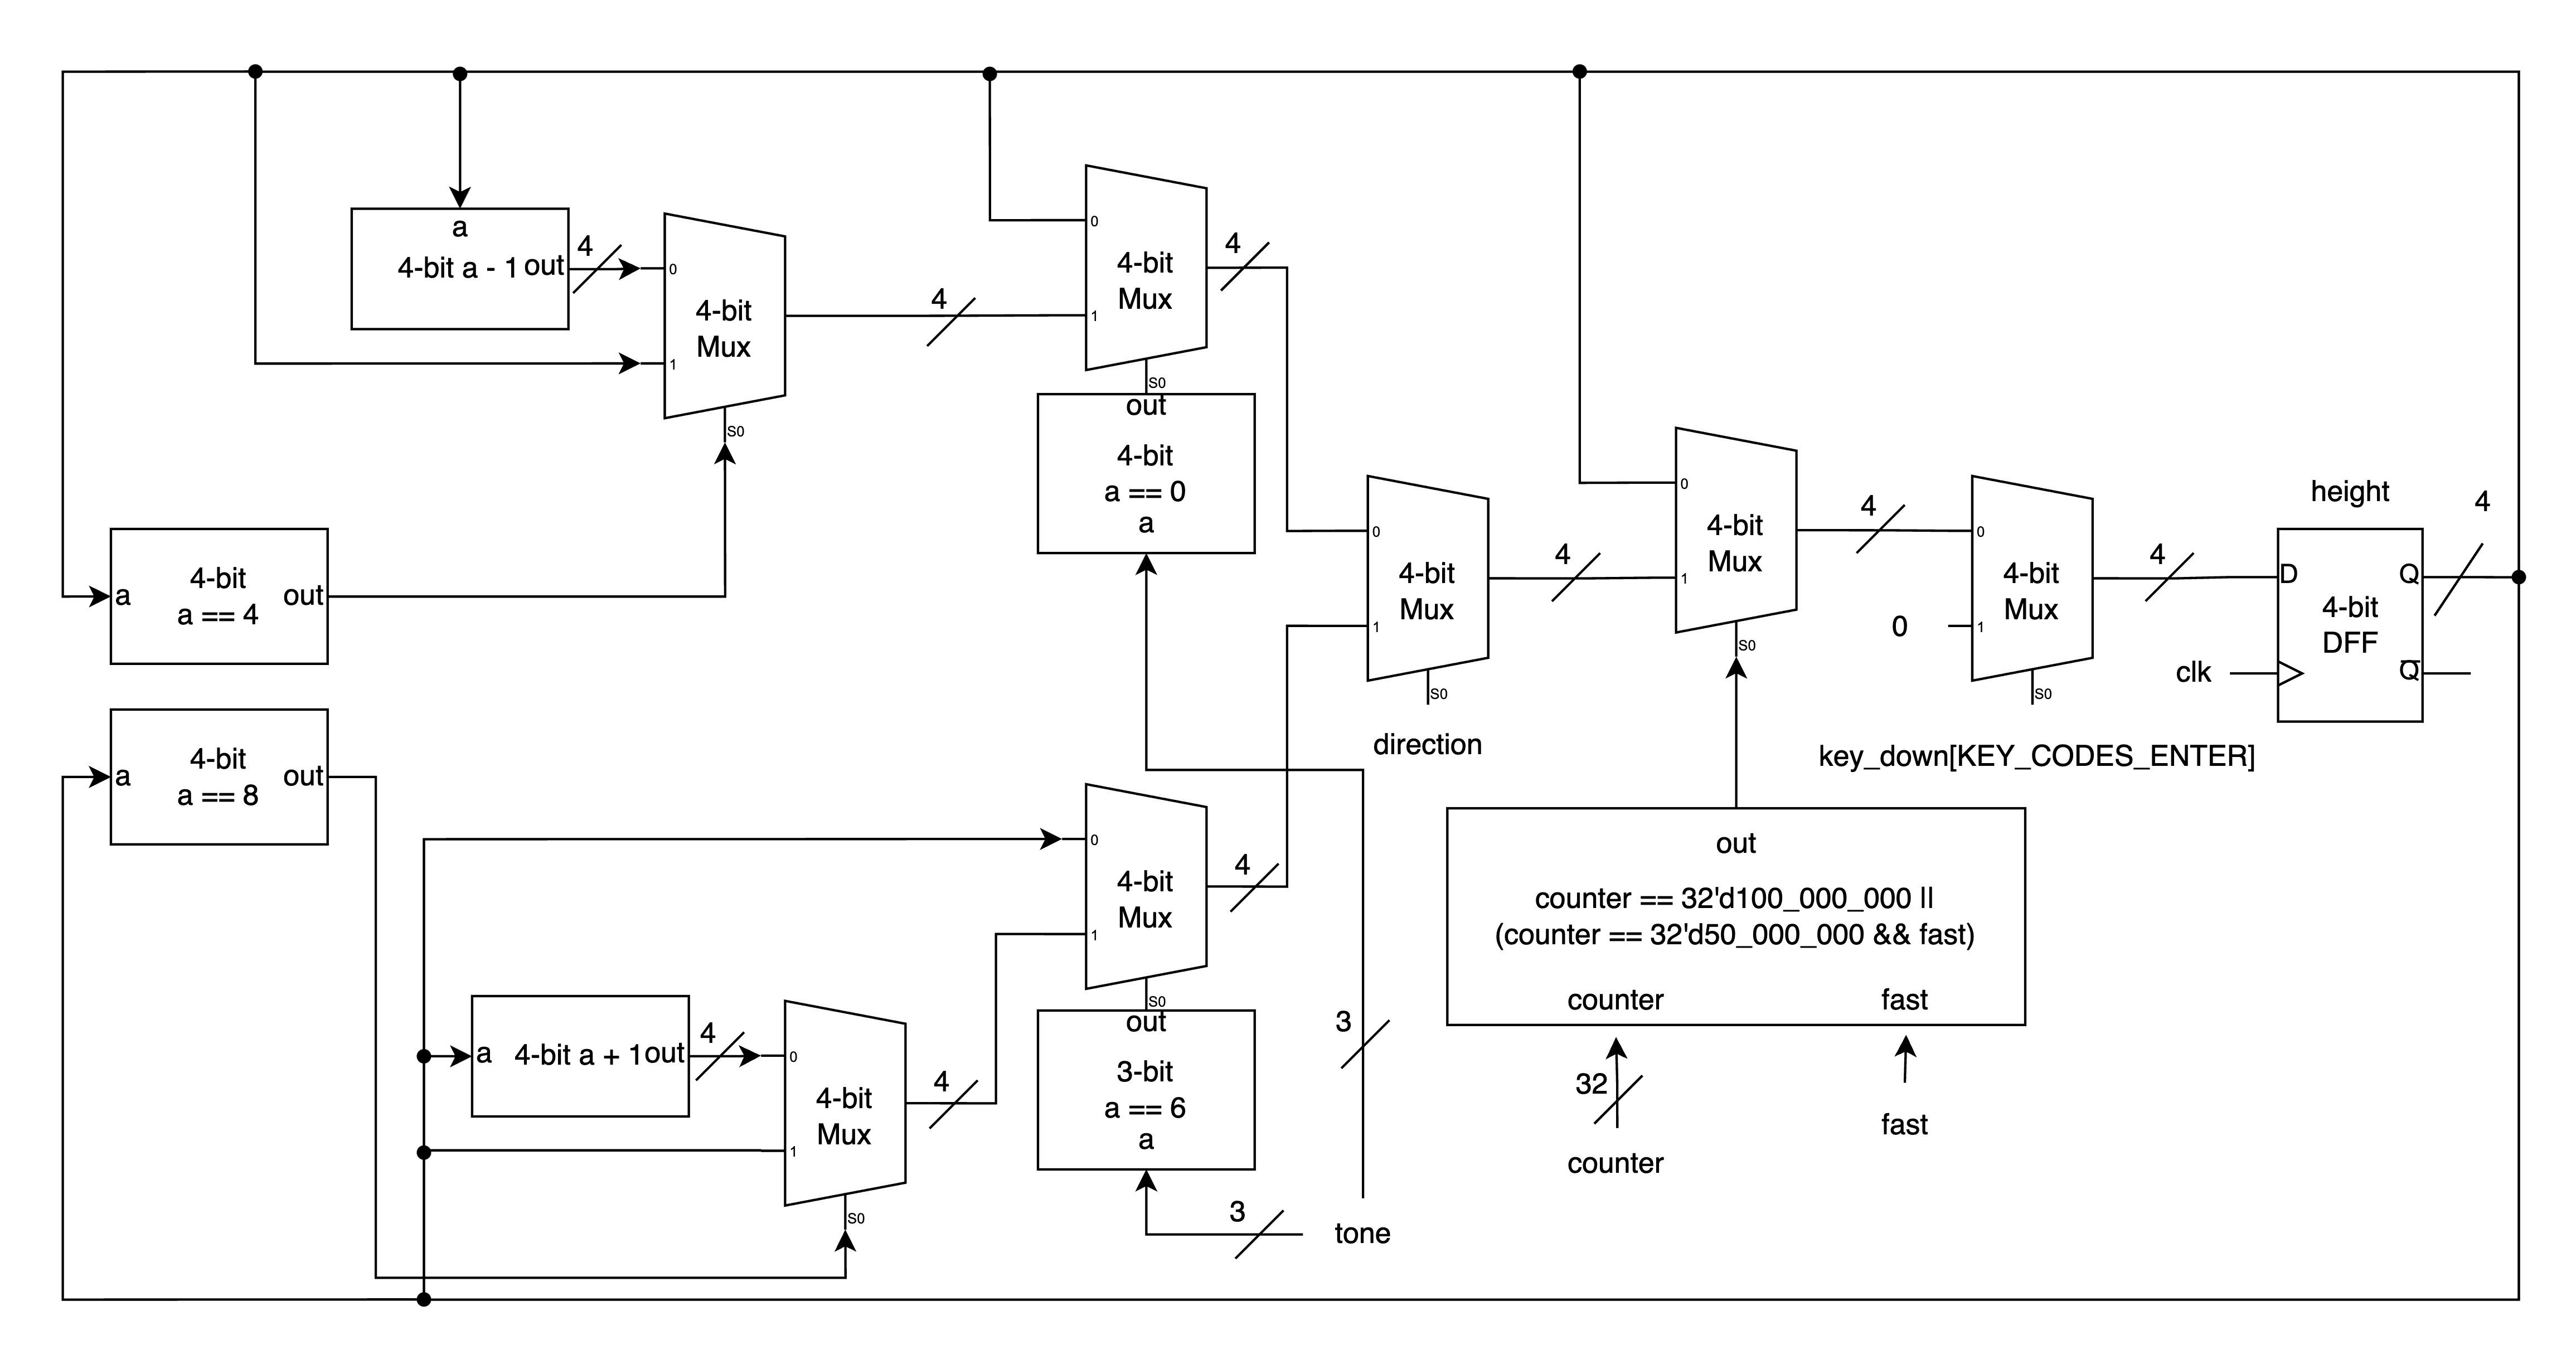
\includegraphics[width=0.8\textwidth]{./img/FPGA1-height.png}
  \caption{FPGA1 Height}
  \label{fig:FPGA1-height}
\end{figure}


最後,只要將 tone, height 輸入到 Decoder 中,得到對應的頻率後輸入至音訊控制模組,就完成了這題的音階控制。\
下圖展現的是相關參數的連接方式:

\begin{figure}[h!]
  \centering
  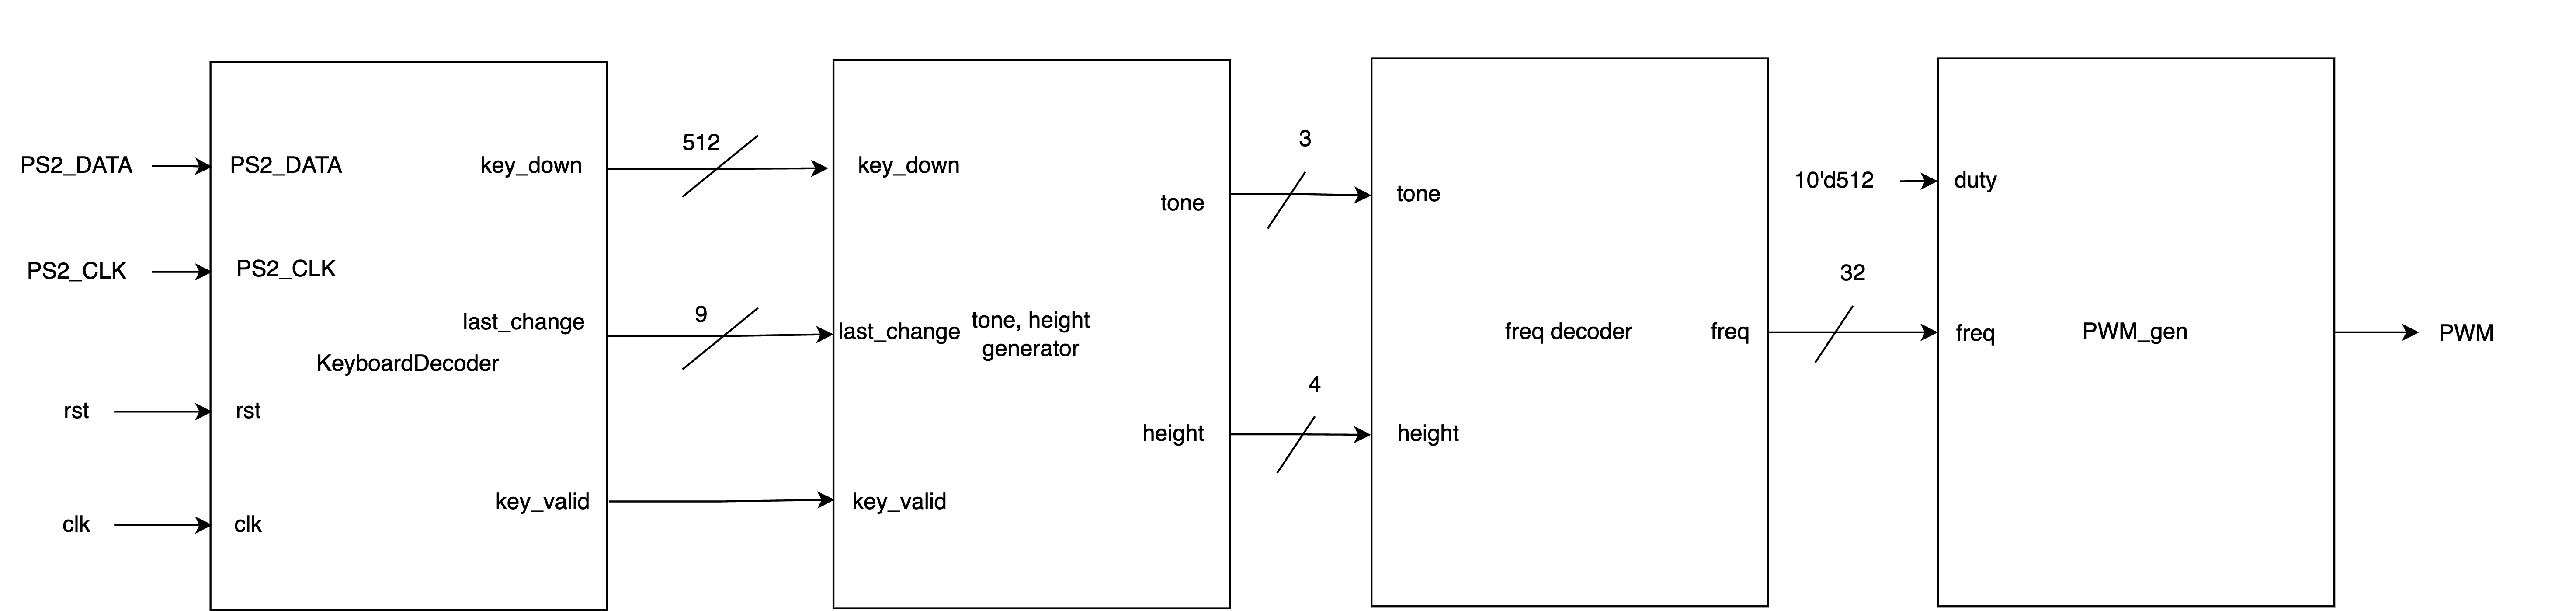
\includegraphics[width=0.8\textwidth]{./img/FPGA1-all.png}
  \caption{FPGA1 Connect}
  \label{fig:FPGA1-connect}
\end{figure}

\newpage
\section{FPGA2: vending maching}
這題要在 FPGA 上實作一個自動販賣機,有三種商品:
\begin{itemize}
  \item Coffee: 80 元
  \item Coke: 30 元
  \item Oolong: 25 元
  \item Tea: 20 元
\end{itemize}

並且有這幾種面值的硬幣,分別對應到板子上的左中右按鈕:
\begin{itemize}
  \item Left: 5 元
  \item Center: 10 元
  \item Right: 50 元
\end{itemize}

並且將板子上的 Top Button 作為 reset 訊號、將 Bottom  Button 作為取消訊號。

\subsection{Implementation}


enable[3:0]: 代表每個商品是否可以購買,透過判斷是否有足夠的錢,以及目前不在 cancel 狀態中來判定:

\begin{figure}[h!]
  \centering
  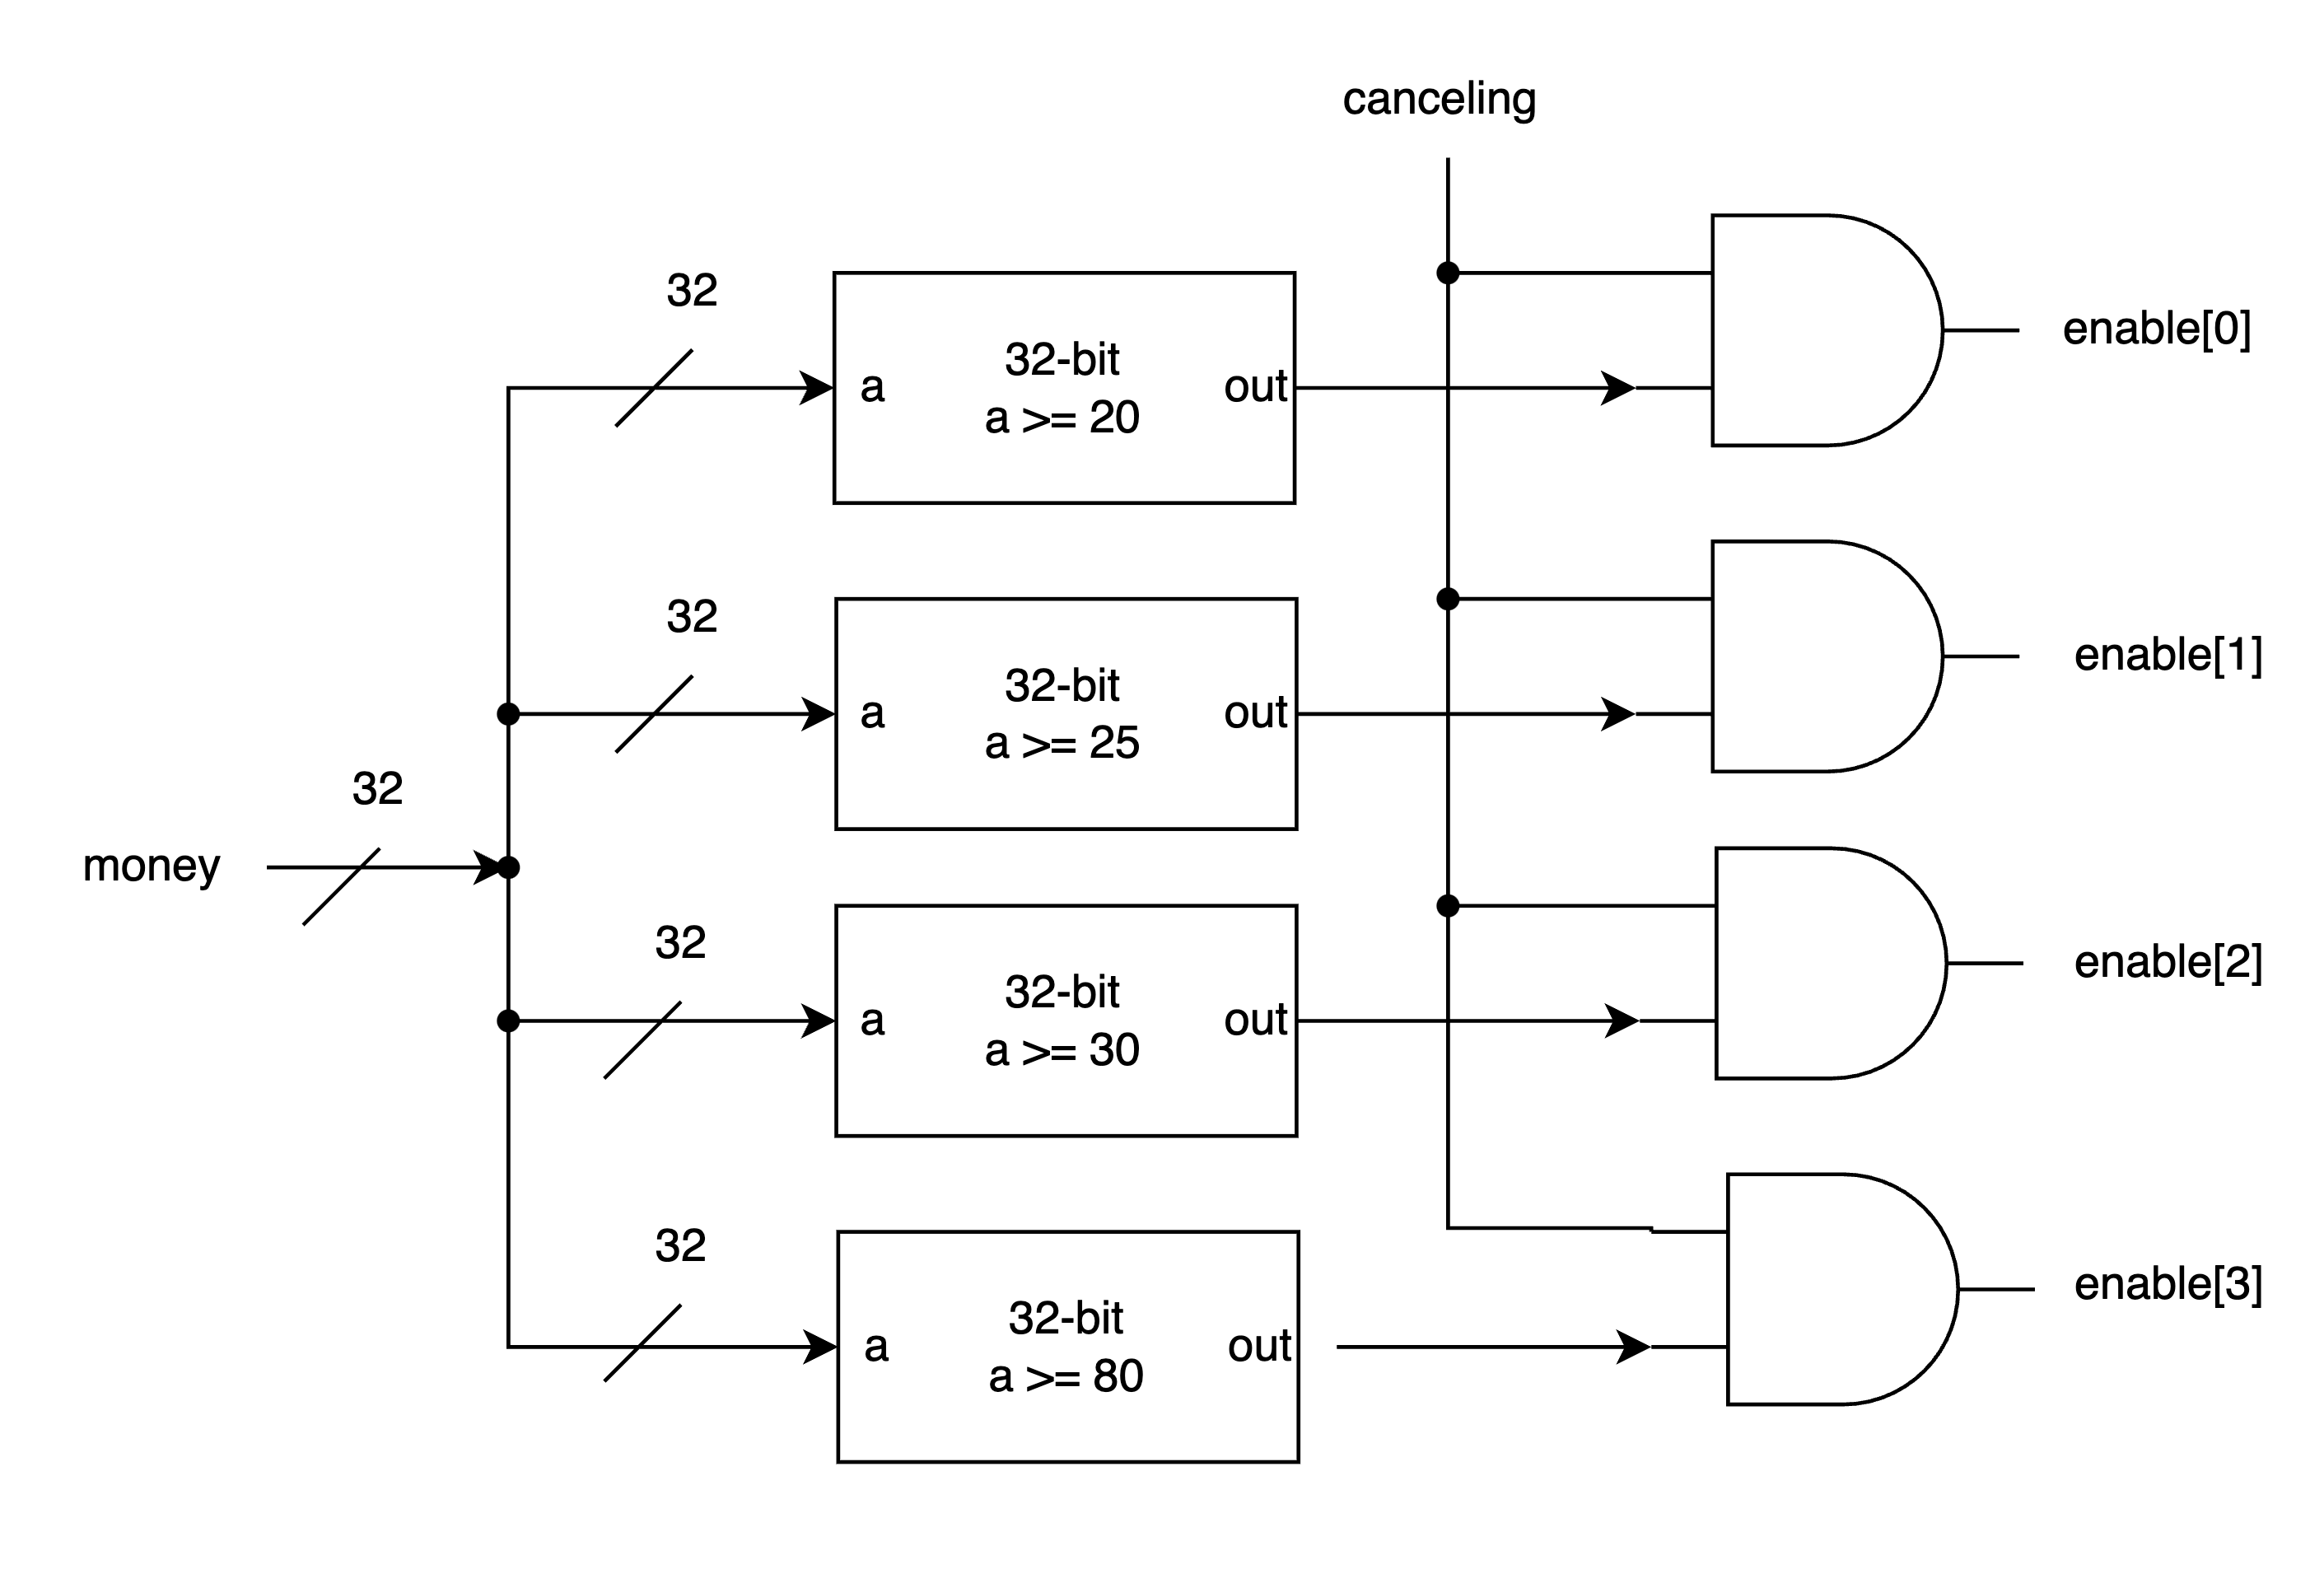
\includegraphics[width=0.8\textwidth]{./img/FPGA2-enable.png}
  \caption{FPGA2 Enable signal}
  \label{fig:FPGA2-enable}
\end{figure}

\newpage

buying: 透過將四個 buy 訊號做 or 運算,來判定是否正在購買:
\begin{figure}[h!]
  \centering
  
\includegraphics[width=0.5\textwidth]{./img/FPGA2-buying.png}
  \caption{FPGA2 Buying signal}
  \label{fig:FPGA2-buy}
\end{figure}

有關取消訊號的部分:

\begin{figure}[h!]
  \centering
  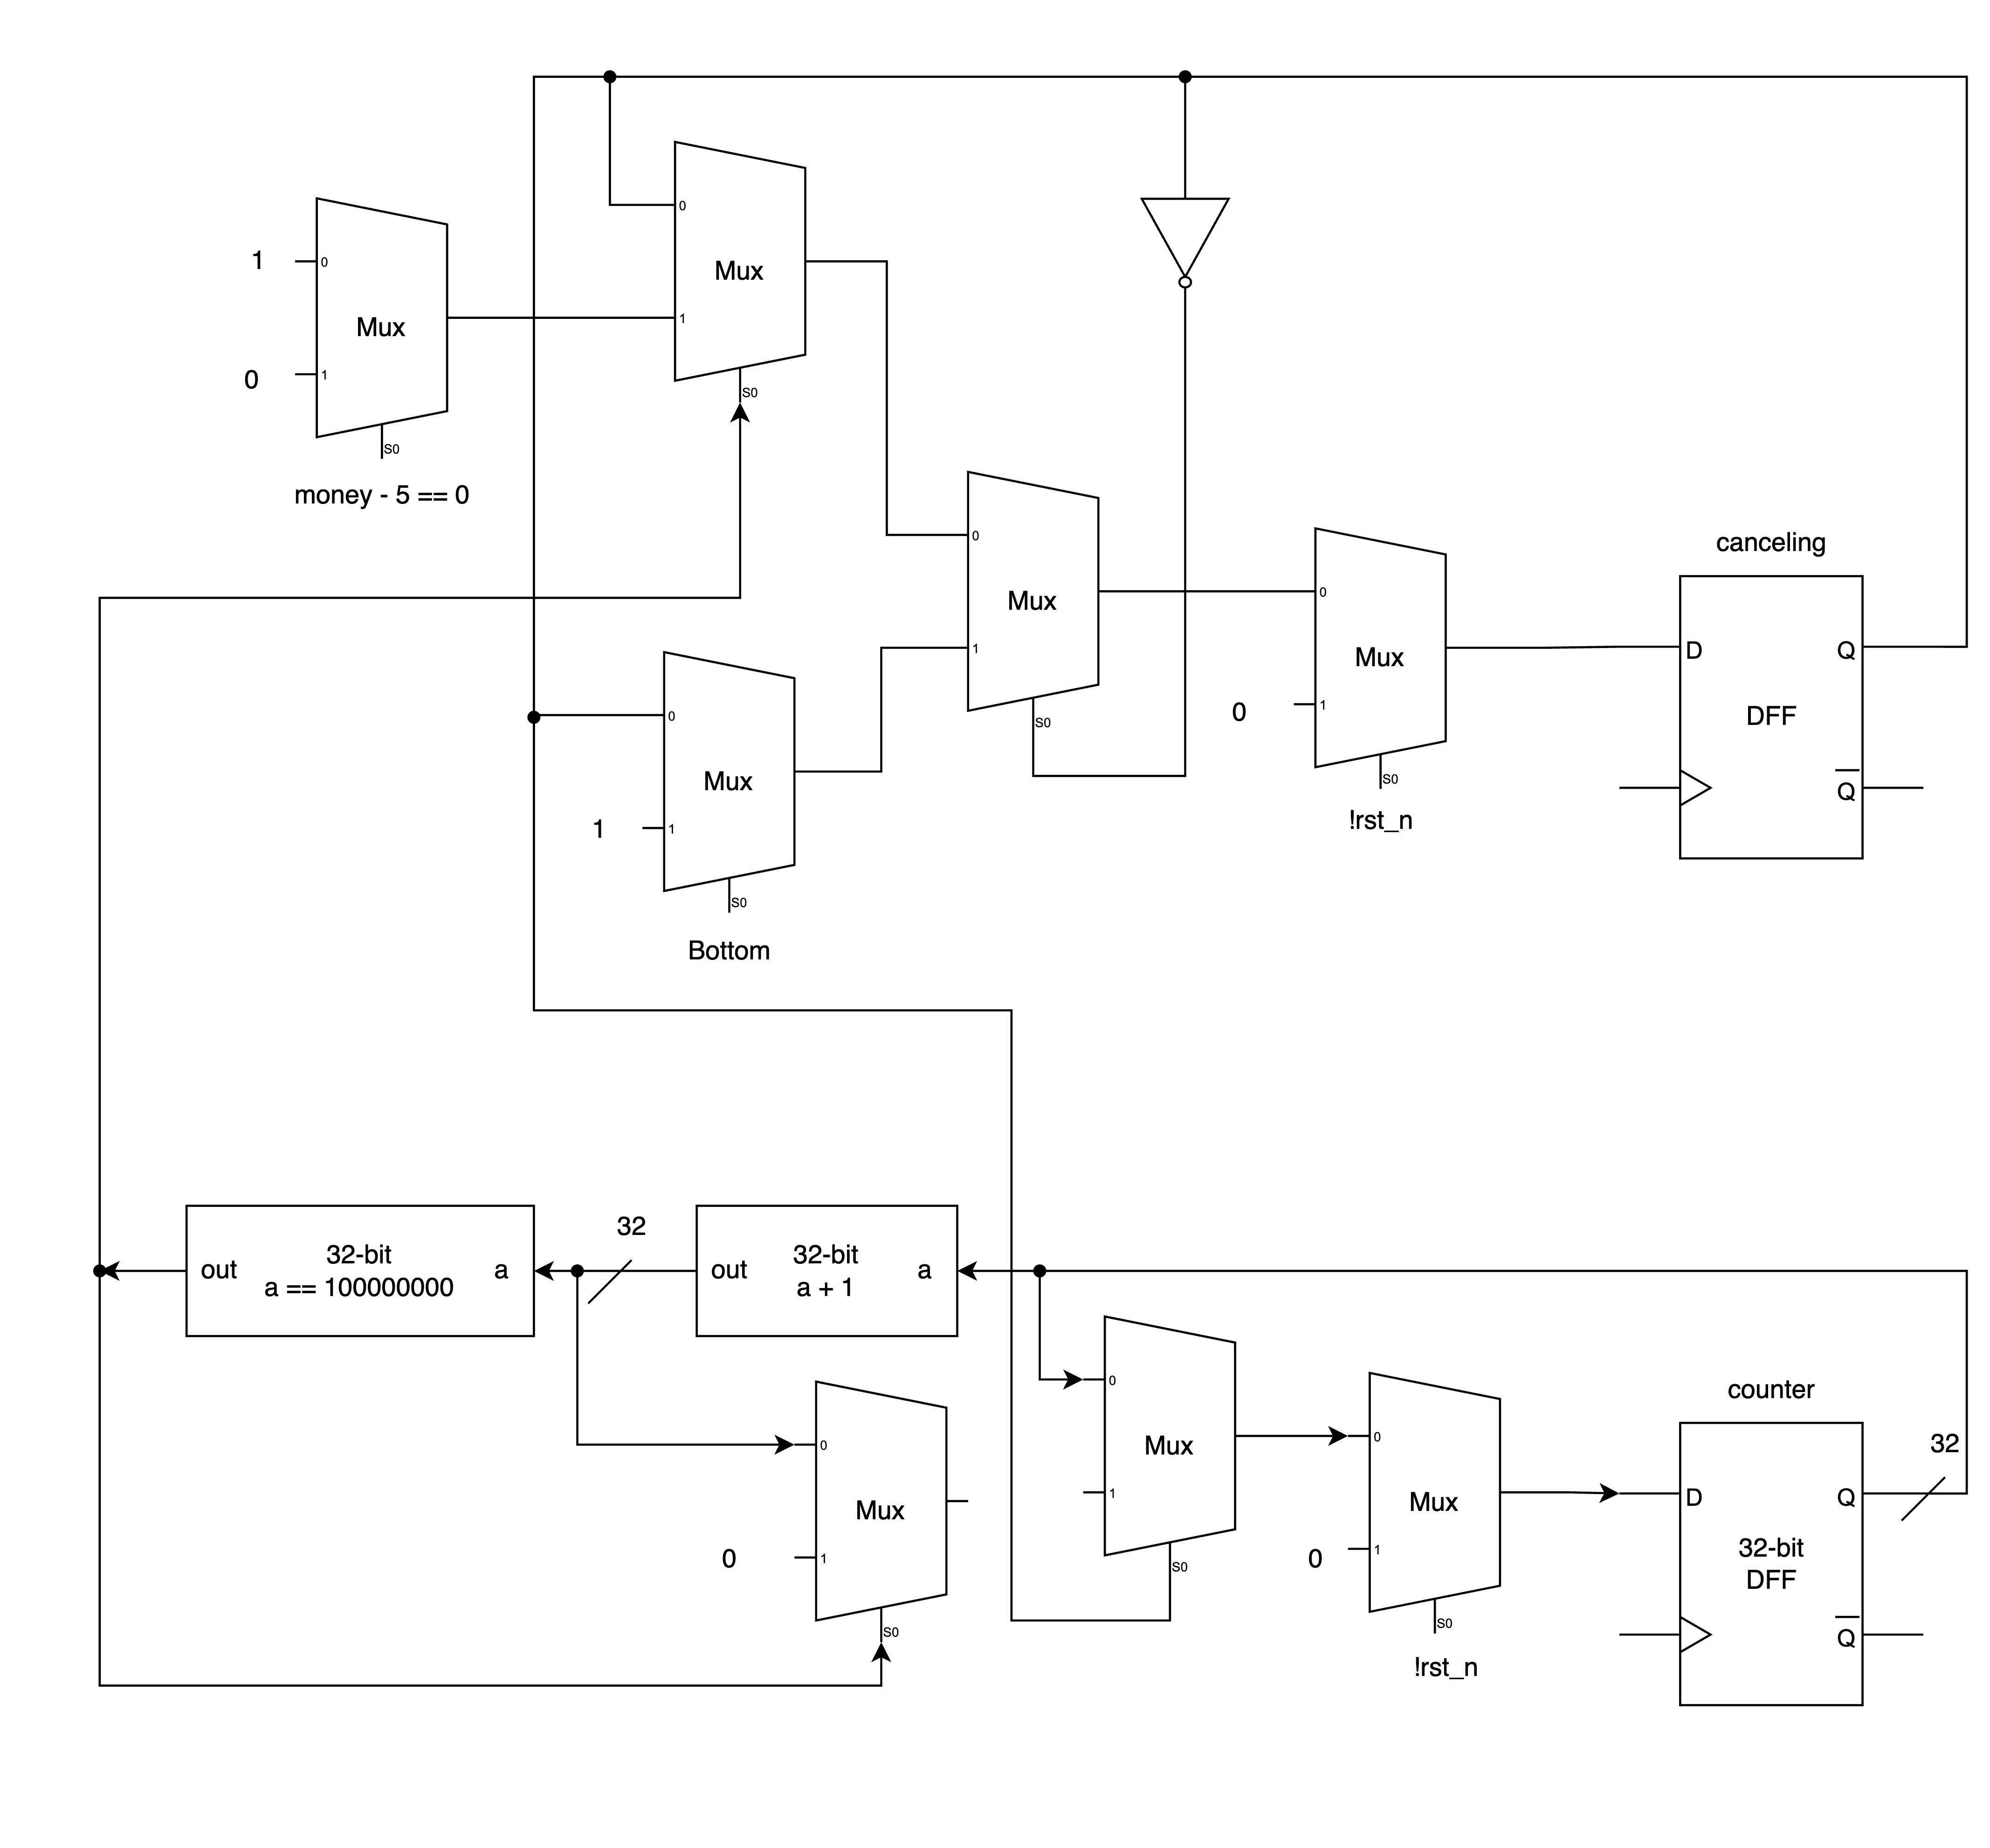
\includegraphics[width=0.8\textwidth]{./img/FPGA2-counter.png}
  \caption{FPGA2 Cancel signal}
  \label{fig:FPGA2-cancel}
\end{figure}

\newpage

將以上訊號接到 state machine 中:

\begin{figure}[h!]
  \centering
  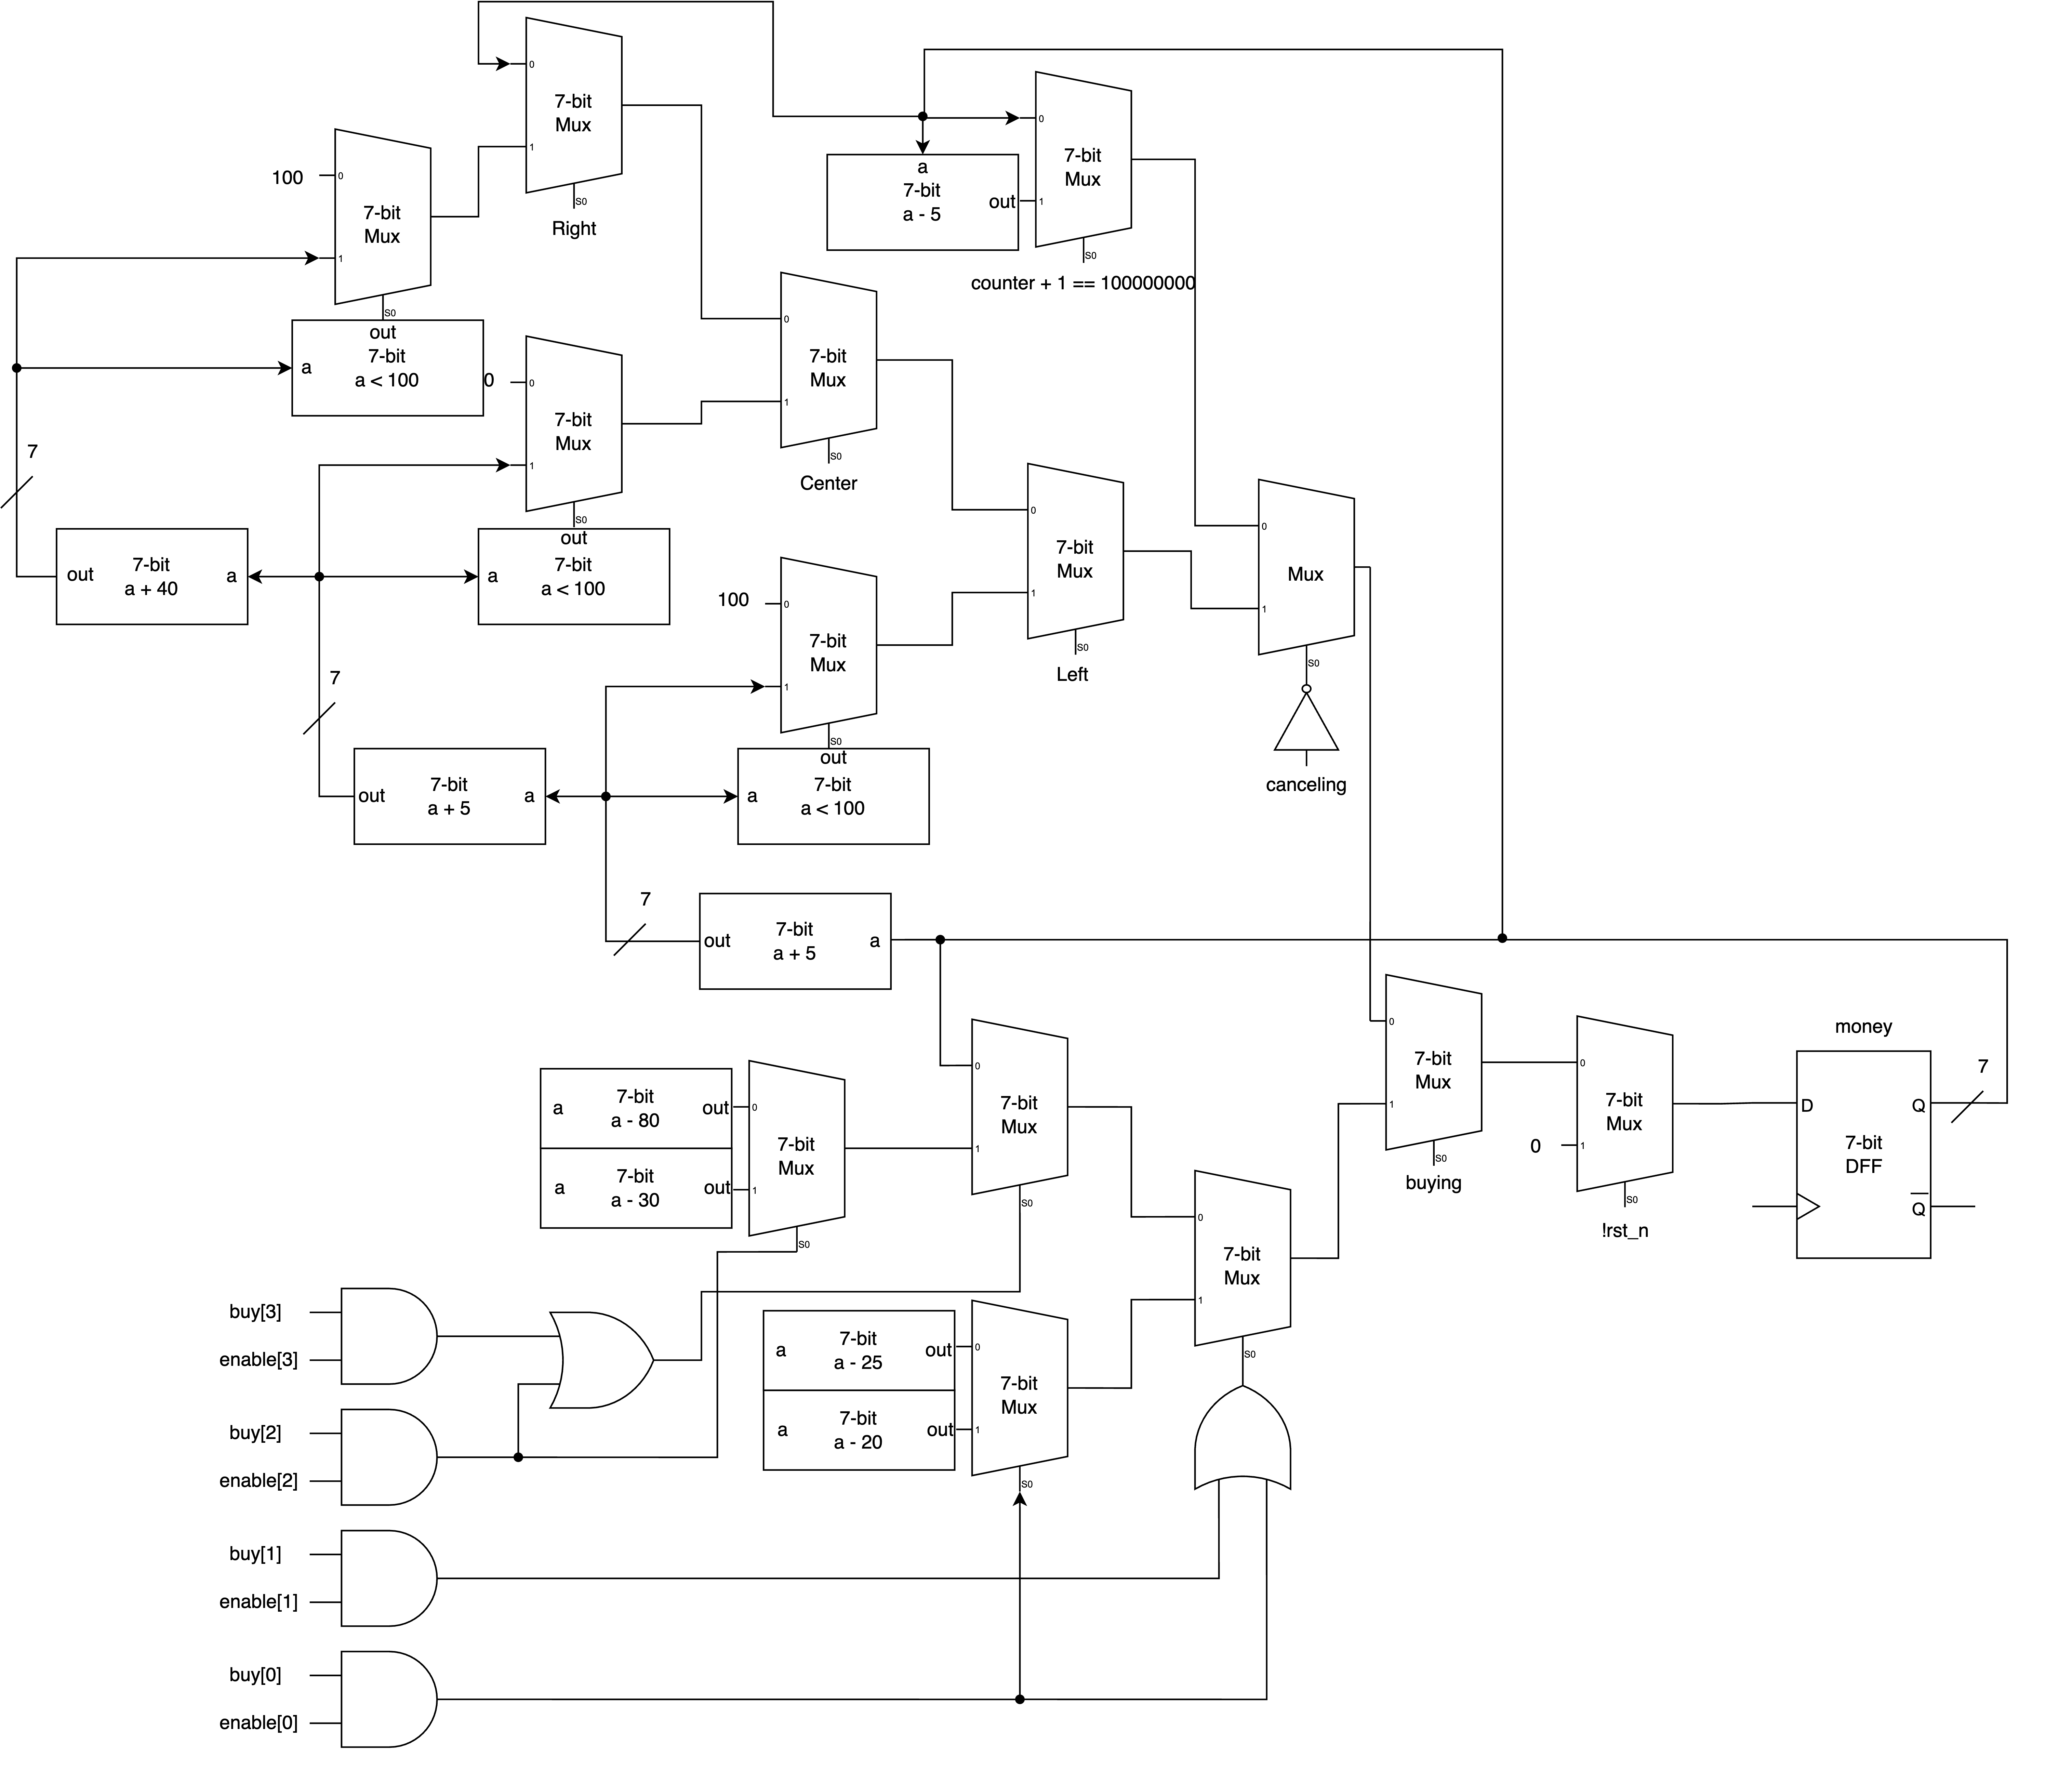
\includegraphics[width=0.9\textwidth]{./img/FPGA2-machine.png}
  \caption{FPGA2 State machine}
  \label{fig:FPGA2-state} 
\end{figure}

\newpage

接著,將 VendingMachine 的輸出接到 NumberDevide 中,計算出三個數字分別要顯示什麼:

\begin{figure}[h!]
  \centering
  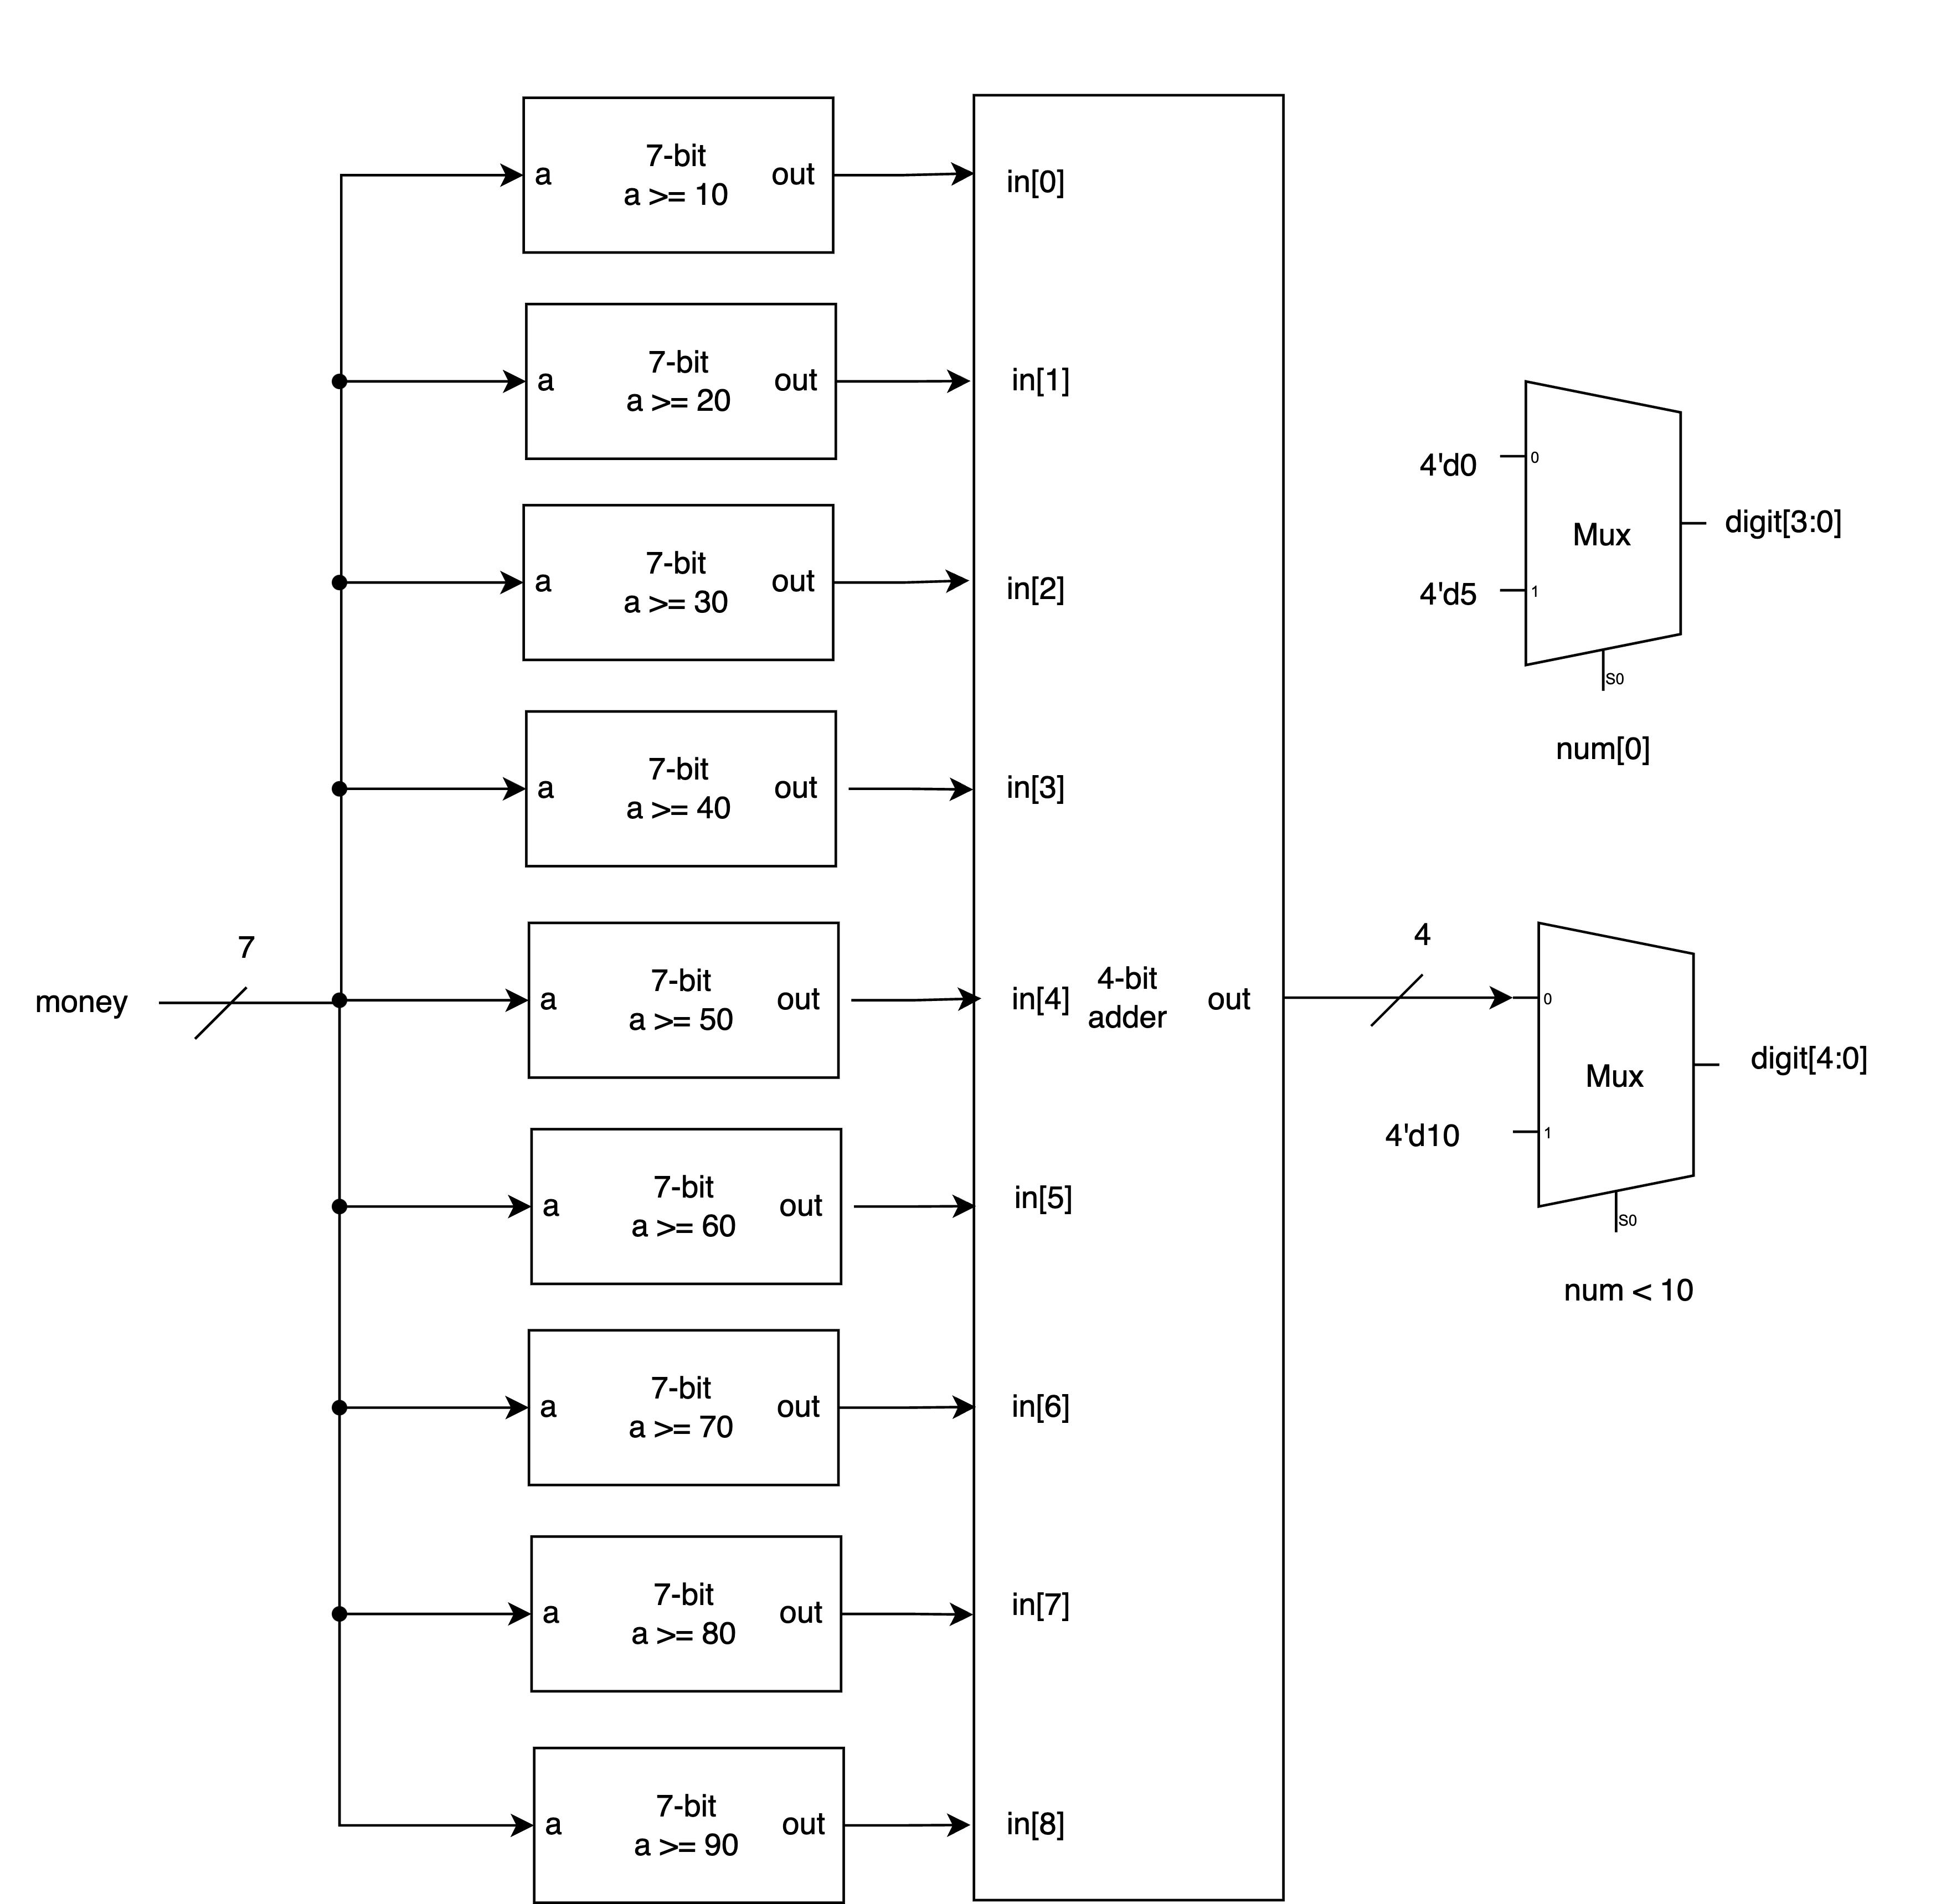
\includegraphics[width=0.9\textwidth]{./img/FPGA2-digit.png}
  \caption{FPGA2 Digit Devider}
  \label{fig:FPGA2-digit}
\end{figure}

最後再將這些訊號接到七段顯示器的輸出控制模組中,就完成了這題的實作。

\newpage

\section{Other}

\subsection{What we have learned}
\begin{itemize}
  \item 這次實作了更多 Finite State Machine,透過多次實作讓我們學習到並建構出一個撰寫 FSM 的 Pattern。\
        使得這次的實作過程比上次都還要順利不少。
  \item 在研究 Booth Multiplier 的過程中,我了解到,其實這個演算法就只是將我們平常加速乘法運算的手法,\
        只是轉成二進位的形式而已。雖然網路上的程式碼沒有理解得很清楚,但因為已經了解概念了,所以還是可以自己寫出來。
  \item 了解到如何在 FPGA 上連接鍵盤,並稍微了解了一下 FPGA 上要怎麼操作 USB 的相關協定,\
        這將對我們 Final Project 的實現方式有很大的幫助。
  \item 實際使用了一些小的音訊裝置組成一個蜂鳴器,比起直接接喇叭,這樣的方式讓我們更認識了喇叭裡面的工作原理,\
        也發現到了,當可變電阻接電過長,有可能因為過熱而導致 FPGA 直接關機。
\end{itemize}

\subsection{分工}
\begin{itemize}
  \item 陳克盈:Q3, Q4, FPGA1, FPGA2
  \item 蔡明妡:Q1, Q2
\end{itemize}

\end{document}


